%% main.tex
%% Copyright 2021 Paulo Henrique De Moura
%
% This work may be distributed and/or modified under the
% conditions of the LaTeX Project Public License, either version 1.3
% of this license or (at your option) any later version.
% The latest version of this license is in
%   http://www.latex-project.org/lppl.txt
% and version 1.3 or later is part of all distributions of LaTeX
% version 2005/12/01 or later.
%
% This work has the LPPL maintenance status `maintained'.
%
% The Current Maintainer of this work is Paulo Henrique De Moura
%
% This work consists of the files ifgw.cls and main.tex
%% Copyright 2005 Paulo Henrique De Moura
%
% This work may be distributed and/or modified under the
% conditions of the LaTeX Project Public License, either version 1.3
% of this license or (at your option) any later version.
% The latest version of this license is in
%   http://www.latex-project.org/lppl.txt
% and version 1.3 or later is part of all distributions of LaTeX
% version 2005/12/01 or later.
%
% This work has the LPPL maintenance status `maintained'.
%
% The Current Maintainer of this work is Paulo Henrique De Moura.
%
% This work consists of the files ifgw.cls and main.tex.
%


\documentclass{ifgw}
\usepackage{amsmath, amssymb}
\usepackage{cite}
\usepackage{caption}
\usepackage{lmodern}
\usepackage{lipsum}
\usepackage{pdfpages}
\usepackage{physics}
\usepackage{siunitx}
\usepackage{microtype}
\usepackage{todonotes}
\usepackage{indentfirst}
\usepackage{booktabs}
\usepackage{multicol}
\usepackage{multirow}
\usepackage{glossaries}
\usepackage{algorithm}
\usepackage{algpseudocodex}


\author{Matheus Melo Santos Velloso}
\city{Campinas}
\supervisor[Supervisor/Orientadora]{Liu Lin}
\cosupervisor[Cosupervisor/Coorientador]{Antonio Rubens Britto de Castro}
\logo[align=left]{Images/unicamp.png}

\title{
    english={Online Optimization of SIRIUS Dynamic Aperture},
    portuguese={Otimização Online da Abertura Dinâmica do SIRIUS},
}

% \subtitle{
%     english={May the Force be with you},
%     portuguese={Que a Força esteja com você},
% }

\institute{
    english={Gleb Wataghin Institute of Physics},
    portuguese={Instituto de Física Gleb Wataghin},
}

\university{
    english={University of Campinas},
    portuguese={Universidade Estadual de Campinas},
}

\backcover{
    portuguese declaration={
        Dissertação apresentada ao \theinstitute~da \theuniversity~como
        parte dos requisitos exigidos para a obtenção do título de
        \uppercase{Mestre em Física}, na área de \uppercase{Física}.
    },
    english declaration={
        Dissertation presented to the \theinstitute[e]~of the \theuniversity[e]~in
        partial fulfillment of the requirements for the de\-gree of
        \uppercase{Master in Physics}, in the area of \uppercase{Physics}.
    },
    version={
        Es\-te tra\-ba\-lho cor\-res\-pon\-de à ver\-são fi\-nal da
        dis\-ser\-ta\-ção de\-fen\-di\-da pe\-lo a\-lu\-no \theauthor~e
        ori\-en\-ta\-da pe\-la Prof. Dr. \thesupervisor.
        % Es\-te tra\-ba\-lho cor\-res\-pon\-de à ver\-são pre\-li\-mi\-nar da
        % te\-se a ser de\-fen\-di\-da pe\-lo a\-lu\-no \theauthor~e
        % ori\-en\-ta\-da pe\-la Dra. \thesupervisor.
    },
    language=english,
}

\loadglsentries{glossary.tex}
\makeglossaries

\begin{document}

\maketitle
\makebackcover
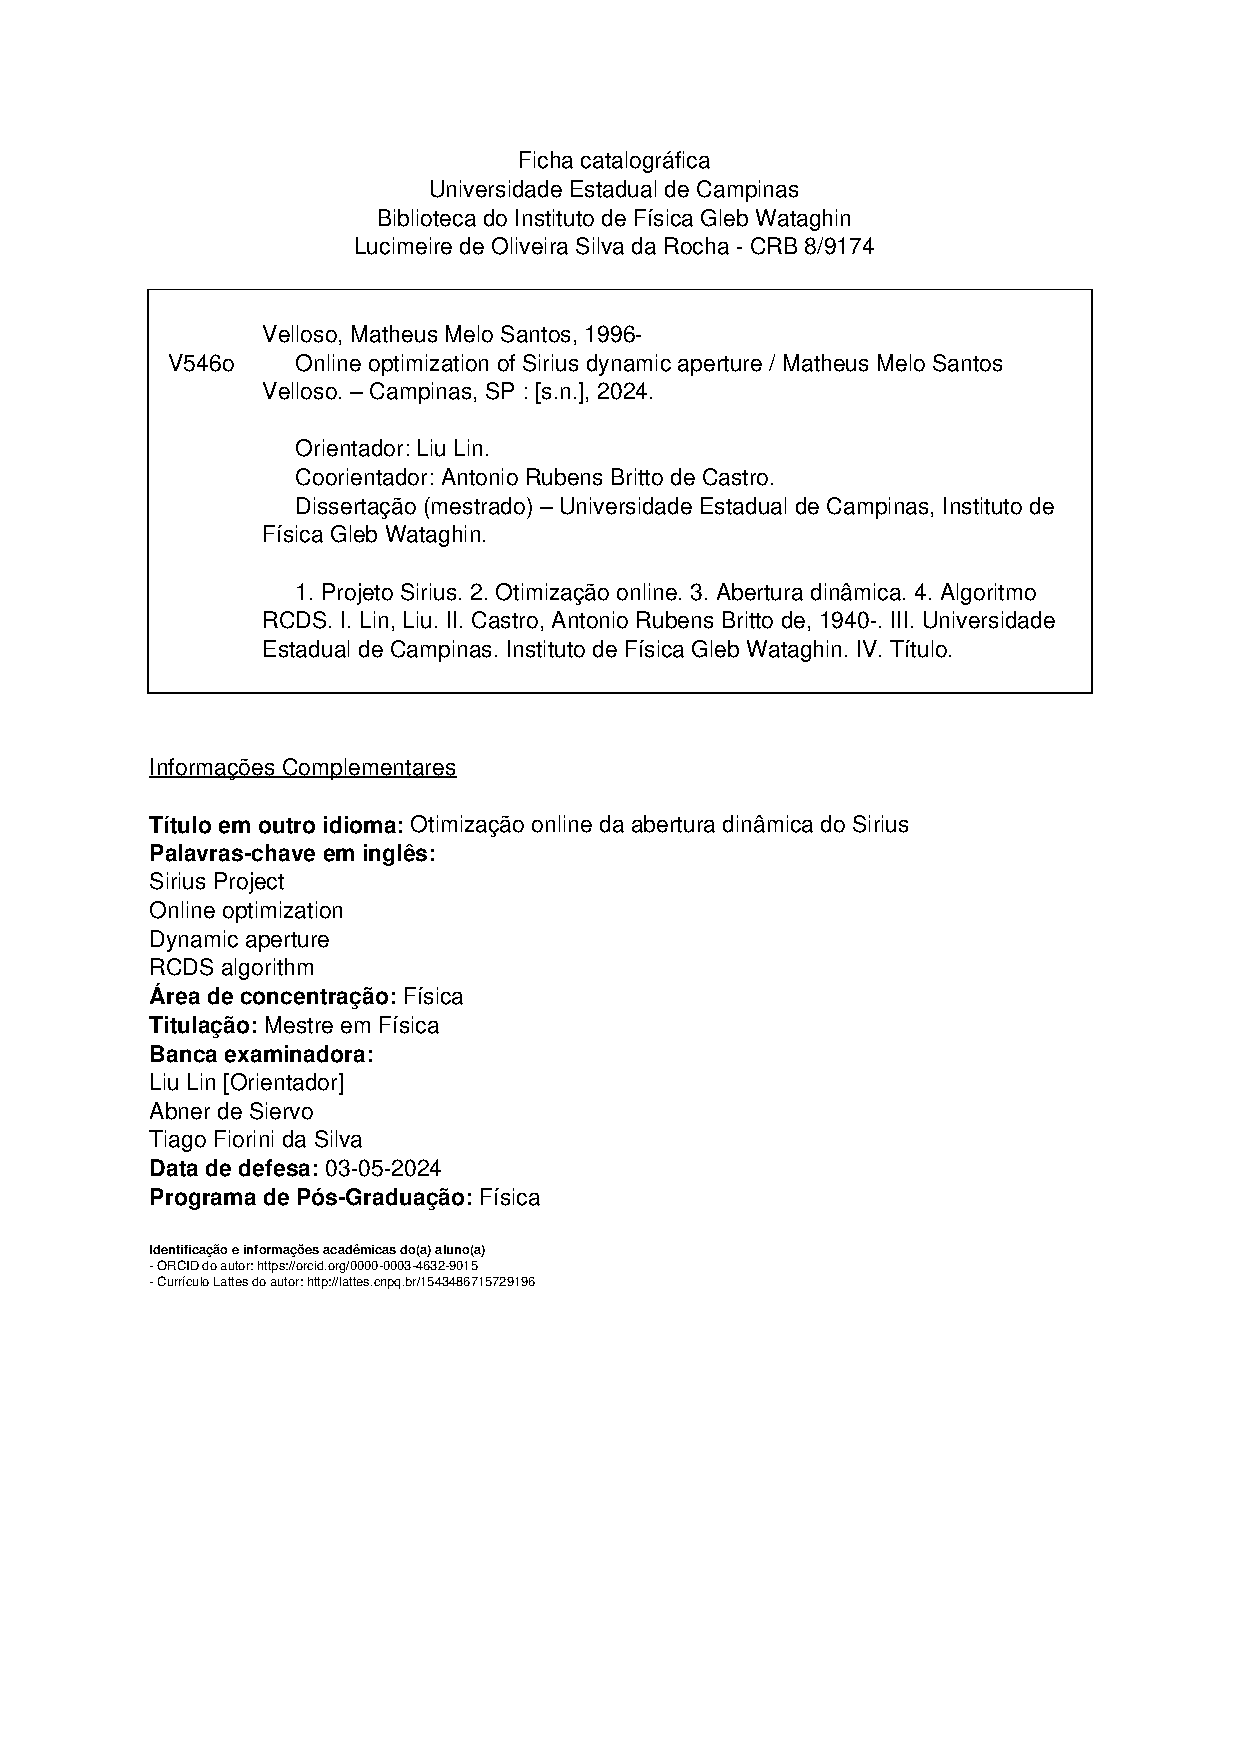
\includepdf[pages=-]{PDFs/ficha_catalografica}
\includepdf[pages=-]{PDFs/folha_de_aprovacao}
% \dedication{To my son, Luke Skywalker.}
% \epigraph{Master Yoda}{May the Force be with you!}


\begin{abstract}[name=Agradecimentos]
    Este trabalho é o resultado do esforço conjunto de diversas pessoas, organizações e instituições, e gostaria de expressar minha profunda gratidão a todos os envolvidos.

    Primeiramente, expresso minha sincera gratidão à minha orientadora, Liu. Sua orientação, supervisão e apoio ao longo deste período foram fundamentais para o sucesso deste projeto. Além disso, sou grato pela oportunidade de participar deste projeto. Esta experiência não apenas enriqueceu minha jornada acadêmica, mas também foi uma valiosa oportunidade de aprendizado, repleta de desafios e crescimento pessoal. Agradeço imensamente por ter tido a chance de trabalhar lado a lado com pessoas tão experientes, inspiradoras, e dedicadas.
    
    Quero estender meu agradecimento aos meus pais pelo seu constante apoio e compreensão e à Juba, cujo amor, carinho e apoio foram fontes de força e conforto.

    Sou grato aos funcionários do CNPEM e do LNLS, e aos colegas do grupo de Física de Aceleradores do LNLS pela colaboração, troca de ideias e momentos de descontração compartilhados durante todo o período de trabalho. Um agradecimento especial ao Fernando pelas discussões valiosas e pela leitura cuidadosa dos materiais produzidos, e ao Murilo pela paciência, disponibilidade e colaboração constante. Também gostaria de expressar minha gratidão ao Ximenes pela liderança inspiradora e compassiva e ao Gabriel pela parceria e amizade.

    Sou grato ao IFGW pela infraestrutura proporcionada, bem como aos professores com os quais tive maior contato e troca. Agradeço ao professor Amir por suas excelentes aulas de mecânica quântica e orientação extraclasse, ao professor Marcos Aguiar pelas aulas de mecânica avançada, e aos professores Diego Muraca, José Brum e Alexandre Fonseca pela orientação durante os programas de estágio docente. Agradeço também aos funcionários da PPG, em especial a Cristina, pelo atendimento proativo e atencioso.

    Gostaria de expressar minha gratidão aos professores e pesquisadores que contribuíram com críticas e sugestões construtivas para este trabalho, em especial ao meu coorientador, Professor Rubens, pela sua presença constante, e aos professores José Brum, Eduardo Granado, Júlio Criginski, Túlio Rocha e Eduardo Miquéles pelas valiosas contribuições durante o desenvolvimento deste projeto.

    Por fim, expresso minha sincera gratidão à CAPES e à FAPESP, por terem sido a fonte de renda que permitiu dedicar-me integralmente a este projeto.
    
    \vspace{1.5cm}

\noindent{\LARGE \textbf{Acknowledgements}}\\
    \vspace*{1.5cm}

    I extend my gratitude to Dr. Xiabiao Huang for his unwavering availability and collaborative spirit. I am truly thankful for the opportunity to have conducted most of experiments outlined in this work in close collaboration with Dr. Huang during his visit to SIRIUS in February 2023. His invaluable insights and support significantly enriched the outcome of our research.

    Furthermore, I am deeply appreciative of Dr. Huang for recommending our work to the organizing committee of the Workshop on Optics Correction and Optimization for Future Colliders. I would also like to express my gratitude to Jackeline Kneitzel, Rogelio Thomaz Garcia, and Frank Zimmerman for their warm hospitality during my attendance at the workshop in Geneva. Lastly, I extend my thanks to all participants of the workshop for their warm reception, valuable feedback, and enriching exchanges. 
\end{abstract}

\begin{abstract}[name=Resumo]
    O acúmulo de feixe no anel de armazenamento do SIRIUS ocorre no esquema de injeção \textit{off-axis}, o qual depende de uma abertura dinâmica (AD) -- a região contemplando oscilações transversais estáveis -- suficientemente grande.
    % Durante a fase de projeto, a AD do SIRIUS foi numericamente otimizada no modelo acelerador usando diversas técnicas, e durante a fase de comissionamento, a rede magnética ótima foi implementada na máquina.
     Antes do trabalho de otimização, a AD do SIRIUS se mostrava suficientemente grande para fornecer uma boa eficiência de injeção, mas também mostrava sinais de que poderia ainda ser melhorada por meio do ajuste fino das forças dos imãs sextupolos, que determinam a AD.
    %   Adicionalmente, o interesse crescente em operar em diferentes pontos de trabalho da ótica, nos quais a AD geralmente é deteriorada, requer o trabalho de otimização online para alcançar valores de eficiẽncia de injeção aceitaveis para a operação.
      Neste projeto de mestrado, o alogritmo \textit{Robust Conjugate Direction Search} (RCDS) para otimização online foi aplicado para otimizar a AD e eficiência de injeção no SIRIUS. Os experimentos também foram realizados em outros pontos de operação, com maiores valores para a parte fracionária das sintonias. Aumentar as sintonias é benéfico para a estabilidade órbita, mas geralmente deteriora a AD, o que requer o trabalho de otimização online para alcançar valores de eficiência de injeção que atendam as demandas da operação. Este trabalho mostra como a otimização online foi bem sucedida para otimizar a AD no ponto de operação nominal do SIRIUS, bem como em um novo ponto de operação, onde melhorias na estabilidade de órbita foram observadas. Os resultados salientam a efetividade desse método em anéis de armazenamento de 4º geração.
\end{abstract}
% Beam accumulation into SIRIUS storage ring occurs in a off-axis scheme, on which the efficiency depends on a sufficiently large dynamic aperture (DA): the region comprising stable transverse oscillations.
% % In the design phase, SIRIUS DA was numerically optimized in the accelerator model using various techniques, and during commissioning, the optimized lattice was implemented in the machine.
%  Prior to optmization, SIRIUS DA was sufficiently large for good injection efficiencies, but showed signs it could be further improved upon fine-tuning of sextupole magnet strengths,
% %  which govern the beam nonlinear dynamics
%  which determine  the DA.
% %  The tuning process is known as Online Optimization and has proven succesful in improving the DA and injection efficiency of SIRIUS, in agreement with the observed outcomes in other machines worldwide.
%  In this master's project, the Robust Conjugate Direction Search Algorithm (RCDS) for online optmization was employed to optimize the DA and the injection efficiency at SIRIUS. Online optimization was also carried out in different optics working points, with higher fractional tunes. Higher tunes are beneficial for improving orbit stability, but the different optics usually deteriorates the DA, requiring online optimization work to achieve injection efficiencies meeting operation demands. This work shows how online optimzation was succesful at optimizing the DA in SIRIUS nominal working point as well as in a new working point where orbit stability improvements were observed. The results highlight the effectiveness of this method in 4th-generation storage rings.

\begin{abstract}
    Beam accumulation into SIRIUS storage ring occurs in a off-axis scheme, on which the efficiency depends on a sufficiently large dynamic aperture (DA): the region comprising stable transverse oscillations.
    % In the design phase, SIRIUS DA was numerically optimized in the accelerator model using various techniques, and during commissioning, the optimized lattice was implemented in the machine.
     Prior to optmization, SIRIUS DA was sufficiently large for good injection efficiencies, but showed signs it could be further improved upon fine-tuning of sextupole magnet strengths,
    %  which govern the beam nonlinear dynamics
     which determine  the DA.
    %  The tuning process is known as Online Optimization and has proven succesful in improving the DA and injection efficiency of SIRIUS, in agreement with the observed outcomes in other machines worldwide.
     In this master's project, the Robust Conjugate Direction Search Algorithm (RCDS) for online optmization was employed to optimize the DA and the injection efficiency at SIRIUS. Online optimization was also carried out in different optics working points, with higher fractional tunes. Higher tunes are beneficial for orbit stability, but usually deteriorate the DA, requiring online optimization work to achieve injection efficiencies meeting operation demands. This work shows how online optimzation was succesful at optimizing the DA in SIRIUS nominal working point as well as in a new working point where orbit stability improvements were observed. The results highlight the effectiveness of this method in 4th-generation storage rings.
\end{abstract}


\listoffigures
\listoftables
\printglossaries
\tableofcontents

\chapter*{Introduction}
\addcontentsline{toc}{chapter}{Introduction}
This dissertation focuses on the work conducted on the SIRIUS storage ring with the objective of optimizing the ring's Dynamic Aperture (DA) and injection efficiency. The text is structured as follows:
\begin{itemize}
    \item The current chapter introduces synchrotron light sources, provides an overview of the SIRIUS project, outlines the main components and subsystems present in electron storage rings, and elucidates the problem addressed in this work;
    \item Chapter 2 delves into the theoretical and scientific background regarding the dynamics of particles in accelerators. It covers topics such as optics functions, tunes, chromatic effects, field errors, perturbations, and the dynamic aperture;
    \item Chapter 3 introduces the online optimization of nonlinear dynamics in accelerators and presents the Robust Conjugate Direction Search (RCDS) algorithm;
    \item Chapter 4 presents the diagnostic tools available for probing the electron beam's motion, current, and other relevant parameters. It also covers technical details on the design of the experiments and measurements, such as the choice of the objective function and the decision variables for the optimization problem;
    \item Chapter 5 presents the results of the online optimization experiments and discusses their significance for the machine operation and stability.
\end{itemize}

\section*{Storage ring-based synchrotron light sources}
\addcontentsline{toc}{section}{Storage ring-based synchrotron light sources}

Synchrotron radiation (SR) is the electromagnetic radiation emitted by charged relativistic particles when accelerated perpendicularly to their motion. The phenomenon was theoretically predicted in the early 1900s when Liénard and Wiechert calculated the retarded potentials for point particles. The first experimental observation occurred at General Electric's synchrotron accelerator, justifying the adoption of the term "synchrotron" in its name \cite{wiedemann_particle_2015}. Synchrotron light is extremely collimated and has a broad spectral distribution, covering from infrared to hard X-rays. These properties make it ideal for imaging experiments in crystallography and spectroscopy across a wide variety of scientific disciplines.

Modern synchrotron light sources primarily rely on two particle acceleration technologies: free-electron lasers and electron storage rings. Here we focus on storage ring-based synchrotron light source facilities. In these facilities, ultra-relativistic electron beams are stored for extended periods in a closed orbit within a chamber in ultra-high vacuum to produce synchrotron light. The beam is maintained in stable orbits by the fields of magnets carefully placed along the ring to provide bending and focusing of the electrons trajectories. It is also periodically influenced by longitudinal standing-wave electric fields in the radio-frequency range, which replenish the energy radiated away in the form of light.

The main figure of merit for measuring the quality of a SR source is the \textit{brightness}\cite{huang_brightness_2013}, defined as the photon flux density in phase space \cite{hettel_challenges_2014}:
\begin{equation}
    B(\omega) = \frac{1}{\Delta \omega/\omega}\frac{F(\omega)}{\Sigma_{x}(\omega)\Sigma_{y}(\omega)},
\end{equation}
where $F(\omega)$ is the photon flux density at energy $E=\hbar\omega$, $\Sigma_{u}$ is the photon beam volume in the $u=x,y$ phase space, and $\Delta\omega/\omega$ is the frequency bandwidth. The photon phase space volume depends on the convolution of the electron beam distribution with the distribution of the photons emitted by a single electron. The latter depends on the photon energy and the emission process, while the former is related to the phase space volume of the electron beam: the \textit{emittance}. The equilibrium beam emittance depends on the magnetic lattice and has units of the transverse phase space areas (size $\times$ angle). Increasing brightness can be achieved by maximizing the photon flux, reducing the electron beam emittances and optimizing the matching between photon and electron beams distribution for maximal convolution \cite{wiedemann_particle_2015}.
%From the perspective accelerator scientists and engineers, in general, the most used figure of merit for synchrotron machines is the emittance rather than brightness.

Synchrotron light sources can be classified based on their brightness and emittance. In the early 1960s, the community interested in SR for imaging experiments obtained it parasitically from high-energy and nuclear physics machines such as DESY and DORIS, in Germany, and ADA, in Italy \cite{simoulin_synchrotron_2016}, marking the era of first-generation synchrotron light sources \cite{liu_towards_2017}. The second-generation machines emerged in the 1980s and consisted on machines designed exclusively for SR production, such as BESSY, DORIS II, DORIS III,  and ELSA, in Germany, SUPERACO, in France, MAX I, in Sweden \cite{simoulin_synchrotron_2016}, and UVX in Brazil.

The 1990s saw a growing demand for higher brightness, leading to the development of third-generation machines \cite{liu_towards_2017}. These machines introduced insertion devices (IDs) such as wigglers and undulators, which consist of a sequence of alternating magnetic fields generally created by an array permanent magnets arranged in a Halbach array. IDs significantly enhance brightness by adding the radiation emitted by many poles. They also allow precise control over the emitted radiation energy and polarization.

Typical emittances for third-generation machines is of the order of units to tens of $\unit{nm}.\unit{rad}$. Most of the currently operating machines pertain to the third-generation, such as ALBA, in Spain, SOLEIL, in France, Diamond, in the United Kindom, and ELETTRA, in Italy \cite{simoulin_synchrotron_2016}.

The era of the fourth-generation of storage rings (4GSR) commenced with the design of the MAX-IV machine in Lund, Sweden, in 2015 \cite{liu_towards_2017,hettel_challenges_2014}. 4GSRs achieved a notable reduction in emittance, reaching sub-$\unit{nm}.\unit{rad}$ values thanks to recent technological advancements in accelerator technology, such as computer simulations, vacuum technology, machining, mechanical alignment, and others  \cite{hettel_challenges_2014,liu_towards_2017}. Following MAX-IV, an upgrade of the ESRF facility, the ESRF-EBS, in France, and the launch of SIRIUS, in Campinas, Brazil, marked significant milestones for the fourth-generation. Today, several 4GSR projects are being planned, designed and constructed around the globe.

\section*{The SIRIUS project}
\addcontentsline{toc}{section}{The SIRIUS project}

SIRIUS is a 4GSR synchrotron light source. It was designed, built, and is operated by the Brazilian Synchrotron Light Laboratory (LNLS), on the campus of the Brazilian Center for Research in Energy and Materials (CNPEM), in Campinas, Brazil. The electron storage ring has $518~\unit{m}$ in circumference and its operating energy is $3~\unit{GeV}$. The natural emittance of the lattice is $250~\unit{pm}.\unit{rad}$. 
% It is expected to reach up to $150~\unit{pm}~\unit{rad}$ with the installation of the machine's definitive IDs \cite{liu_synchrotron_2019}\footnote{SIRIUS is currently operating with provisional IDs for providing light to the first users and allowing scientific commissioning of the beamlines}.

SIRIUS succeeded the first synchrotron light source in Brazil, the UVX machine, which opened to users in 1997 and served the community until its shutdown, in the beginning of SIRIUS commissioning, in August 2019\footnote{The UVX project led to the creation of LNLS, which marked a new model for scientific research in Brazil, based on social organizations under contracts with the Ministry of Science Technology and Innovations. LNLS paved the way for national labs (NL), including labs on bio-sciences (LNBio), nanotechnology (LNNano), and bio-renewables (LNBR), which are also located at the CNPEM campus.}\cite{liu_synchrotron_2019}. The SIRIUS project started in 2009, initially planned and designed as a third-generation machine. By 2012, the project evolved into that of a 4GSR \cite{liu_synchrotron_2019}. Building construction was finished in 2018, the LINAC and Booster commissioning soon followed. In November 2019 the first beam was stored in the storage ring.

SIRIUS finished the Phase-0 commissioning in 2022 and since March 2023 is receiving the first external users. At the time of this writing, \todo{check this info} it has 6 operating beamlines, 4 beamlines in commissioning and 4 under construction and installation. It is currently storing $100~\unit{mA}$ current, with frequent beam injections throughout the day, a scheme known as ``top-up'' mode. SIRIUS is expected to achieve $350~\unit{mA}$ current when the system of two superconducting radio-frequency cavities and the third-harmonic cavity are installed \cite{liu_status_2022,liu_status_2023}.


....



Presently, SIRIUS stands as the most complex scientific infrastructure ever constructed in Brazil, aiming to position the country at the forefront of global leadership in synchrotron light science and technology. It has the capacity to host up to 40 beamlines and as of the time of this writing, SIRIUS is the sole fourth-generation synchrotron light source in the southern hemisphere and one of merely three 4GSRs in operation across the globe.

\section*{Physics of electron storage rings: an overview}
\addcontentsline{toc}{section}{Physics of electron storage rings: an overview}

Typical systems comprising a storage ring synchrotron light source facility include:
\begin{itemize}
    \item an injection system: including the electrons source, beam transport lines, the linear accelerator and the booster synchrotron accelerator. At SIRIUS, the linear accelerator provides the booster with a $150~\unit{MeV}$ beam. The booster further ramps the beam energy up to $3~\unit{GeV}$, which is the storage ring operation energy;
    \item storage ring: where the ultra-relativistic beam of electrons is kept in stable orbits for hours within the vacuum-chamber, producing synchrotron light at the bending magnets and insertion devices;
    \item beamlines which steer the photon beams towards the experimental cabins where samples are placed for the experiments based on light-matter interaction, such as spectroscopy, crystallography, tomography and others.
\end{itemize}
A schematic view of the SIRIUS building is shown in Fig.~\ref{fig:sirius_layout}.
\begin{figure}[tb]
    \centering
    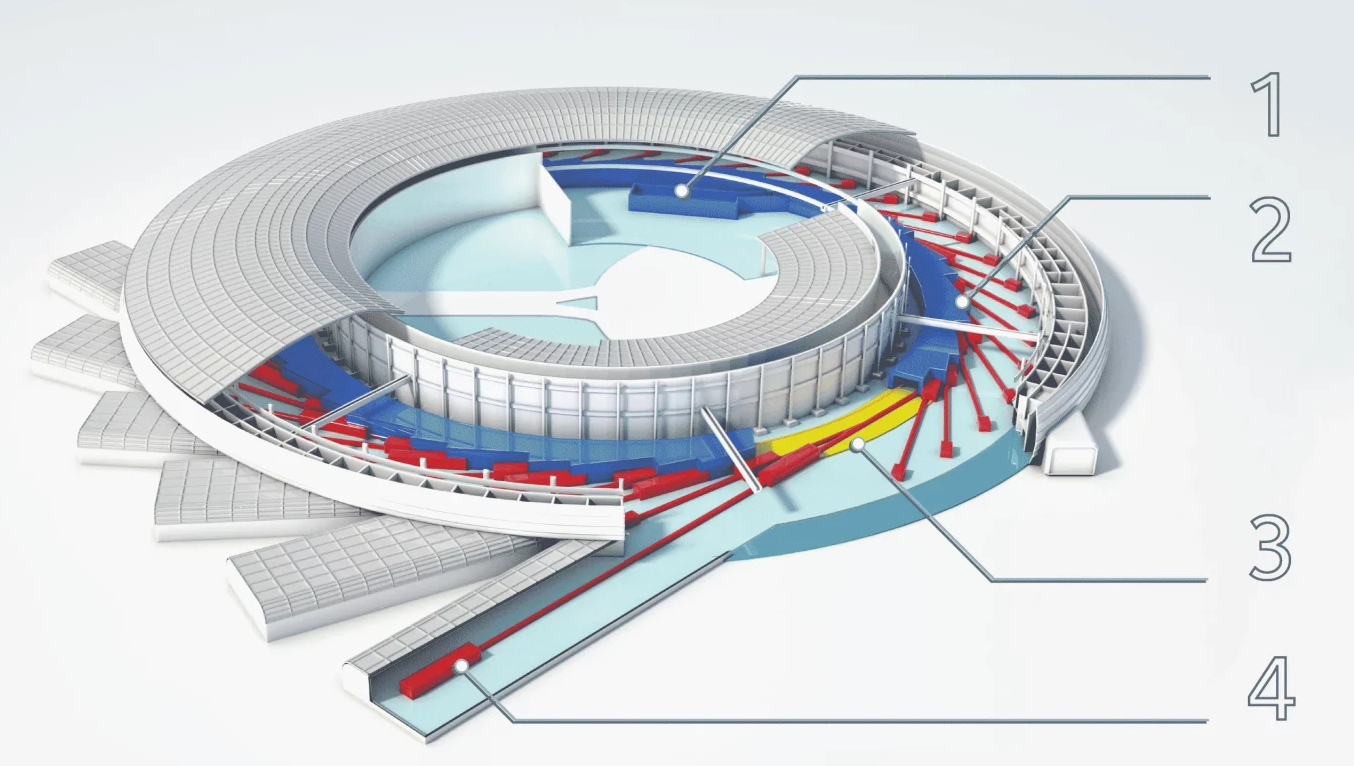
\includegraphics[width=0.8\textwidth]{Images/sirius_facility.png}
    \caption[Schematic view of the SIRIUS installations.]{Schematic view of the SIRIUS installations. 1) Linear accelerator (LINAC); 2) Concrete tunnel housing the booster accelerator and the storage ring; 3) storage ring; 4) beamlines. From \href{https://lnls.cnpem.br/sirius/como-funciona-o-sirius/}{LNLS website}.}
    \label{fig:sirius_layout}
\end{figure}

\begin{figure}[tb]
    \centering
    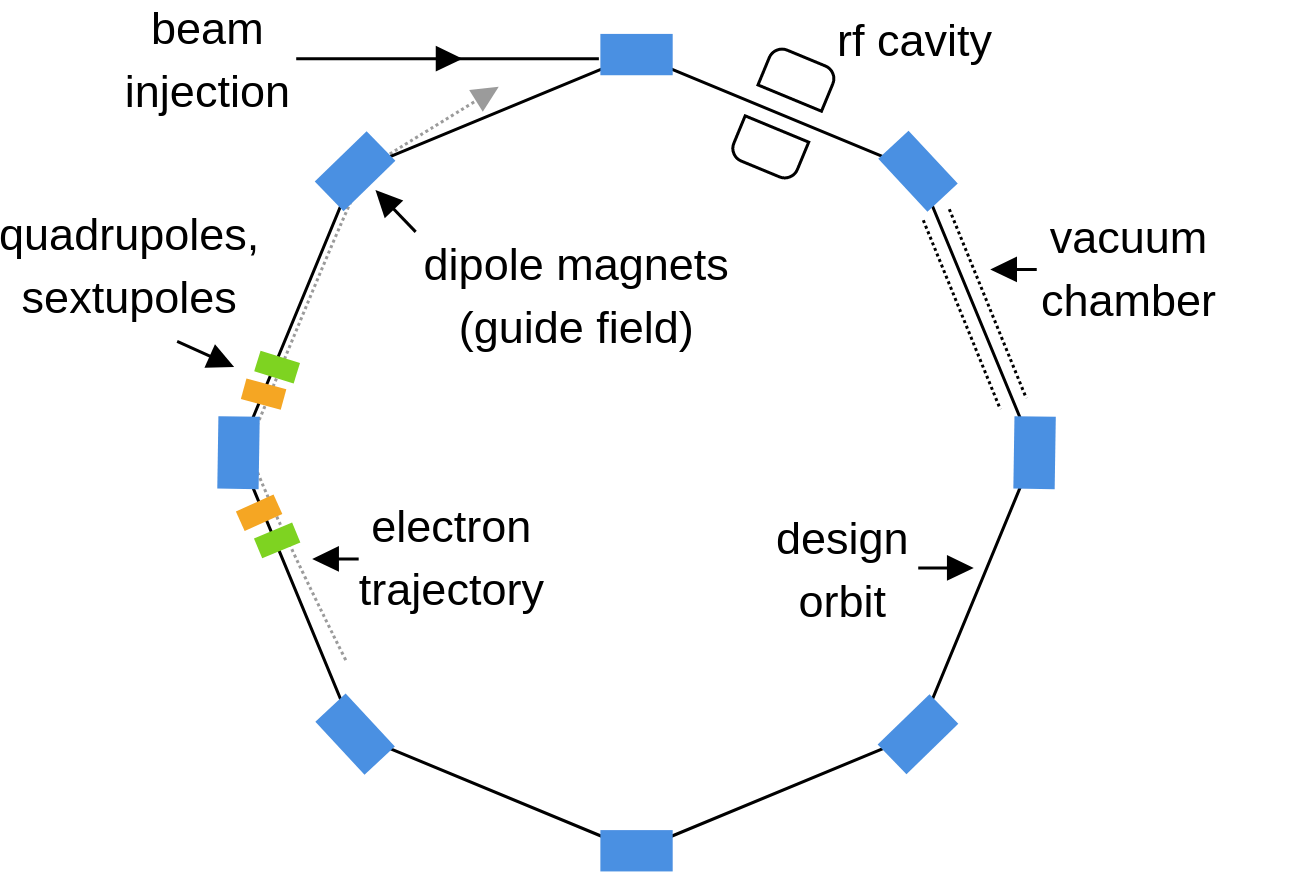
\includegraphics[width=0.6\textwidth]{Images/storage_ring.png}
    \caption[Storage ring typical configuration.]{Storage ring typical configuration. Inspired by ref.~\cite{sands_physics_1969}}
    \label{fig:storage_ring}
\end{figure}
Figure~\ref{fig:storage_ring} outlines the typical layout of a synchrotron storage ring. The electron beam is stored within a vacuum chamber, where the individual electrons oscillate in proximity to a reference closed orbit, under the influence of magnetostatic fields from an array of multipolar magnets --the lattice, and also time-dependent fields from the radio-frequency (RF) cavities. The orbit circumference is determined by the strengths of the deflection magnets, the dipoles, and the operational energy of the beam.

A pure dipole magnet provides a uniform and homogeneous magnetic field perpendicular to the facility floor and bends the electron's trajectory in the plane parallel to the floor. The field profile of a dipole magnet is depicted in the left-side sketch of Fig.~\ref{fig:magnets_fields}. Imagining a beam directed inward toward the screen, the trajectory will be bent to the right. For trajectories resulting in a closed orbit, the overall bending angle provided by the dipoles along the entire ring must equal $2\pi$ radians.

To maintain electrons in close proximity to the reference orbit, focusing of the trajectories is required. Focusing is attained by employing gradient fields, primarily generated by quadrupole magnets at SIRIUS. The strength of such fields increase linearly with deviations from the closed orbit, which lies in the magnet's center. Gradient fields effectively act as restoring spring forces. The magnets poles and the field profile of a quadrupole magnet are depicted in the center sketch of Fig.~\ref{fig:magnets_fields}.

Focusing and deflection are energy-dependent, which means small deviations from the nominal operating energy can result in a enlarged or reduced orbit and on differential focusing at the gradients. The former effect is a dispersion effect, while in the latter, drawing an analogy from geometric optics, the beam's focusing behavior at the "lens" (quadrupoles) depends on its "color" (energy). To correct for these chromatic aberrations the sextupole fields serve as corrective lenses. They introduce geometric aberrations to counteract the chromatic ones, resulting in approximately uniform, energy-independent focusing, up to the linear approximation. The magnets poles and the field profile of a sextupole magnet are depicted in the right sketch of Fig.~\ref{fig:magnets_fields}.

Besides dipoles, quadrupoles and sextupoles, additional dipole actuators magnets for orbit/trajectory correction and pulsed magnets for beam injection can also be found in the ring.
\begin{figure}[htb]
    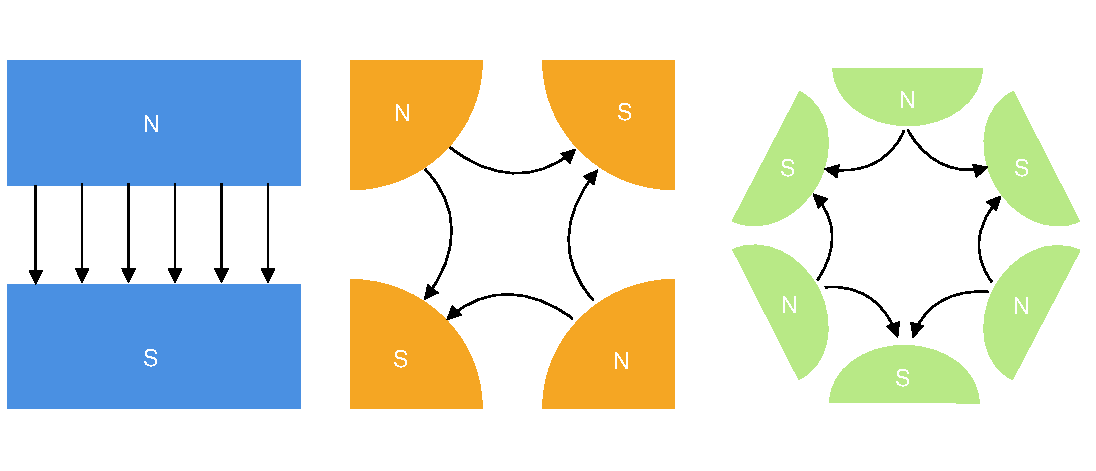
\includegraphics[width=\textwidth]{Images/magnets.pdf}
    \caption[Schematic representation of the magnets comprising SIRIUS lattice and their fields profile.]{Schematic representation of the magnets comprising SIRIUS lattice and their fields profile. From left to right: dipole magnet, quadrupole magnet and sextupole magnet.}
    \label{fig:magnets_fields}
\end{figure}
%As mentioned previously, a storage ring is designed to confine bunches of electrons and steer them along a reference closed orbit. The orbit is defined by the bending magnets, the dipoles. The trajectories consist on oscillations about the closed orbit, and focusing of such oscillations toward the closed orbit is provided by gradient fields, mostly coming from quadrupole magnets. Additionally, to correct chromatic aberrations in the beam's motion, i.e. a dependence of focusing with the beam's energy, and guarantee correct focusing despite energy deviations from the nominal value, sextupolar magnetic fields are also introduced, providing fields depending qudratically on the deviations from the nominal orbit. These fields introduce strong nonlinearities in the dynamics.

When having its trajectory bent at the dipoles and insertion devices,
%\footnote{Insertion devices (IDs) consist on arrays of magnetic blocks arranged to provide additional deflection of the beam's trajectory for the production of synchrotron radiation. IDs allow for fine-tuning of the fields and as consequence of the characteristics of the emitted readiation, such as the energy and polarization.}
the beam loses energy in the form of synchrotron radiation. To avoid inward spiraling and maintain the beam stored, the energy lost must be replenished. To achieve this, radio-frequency (RF) cavities are placed along the ring to provide oscillating electric fields along the longitudinal direction. The work done in the beam by the fields restore its energy.

The radiated photons are emitted in a narrow cone with angular aperture of $1/\gamma$, $\gamma$ being the relativistic Lorentz factor ($\sim 6000$ at SIRIUS storage ring). The photons carry away a fraction of the beam's momentum in both the longitudinal and transverse directions. However, when passing through RF cavities, only momentum in the longitudinal direction is replenished. The combined effect of radiating photons and passing through RF cavities leads to an overall damping of the transverse oscillations amplitudes.

On the other hand, the quantum nature of the emitted radiation leads to the excitation of transverse oscillations, an effect known as quantum excitation. When a photon carries away energy, it depletes the electrons energy by the same amount. It thus changes the reference orbit of the electron because of the dispersion effect, inducing oscillations. Additionally, coupling on the transverse plane and intra-beam scattering events can lead to the excitation of transverse oscillations, enlarging the beam size.
%Additionally, the very fact that radiation is emitted within a finite angular aperture means that, by momentum conservation, the emission of a photon is accompanied by a transverse recoil. These two mechanisms are responsible for the excitation of transverse oscillations. 
Eventually, equilibrium between radiative damping and transverse excitations is achieved, leading the beam size to reach a stationary value

Each degree of freedom of the beam defines an acceptance, which establishes limits on the dynamical variables. Exceeding these limits can result in unstable, unbounded motion, and eventually, beam losses. The most apparent form of acceptance is the transverse acceptance, since the beam motion is bounded by a vacuum chamber, and colliding with the chamber's physical aperture leads to losses. Additionally, the beam has an energy acceptance, representing a tolerance for energy deviations from the nominal value. Exceeding this tolerance can lead to a sub-optimal energetic balance when passing at the RF cavities. On the span of several turns, the energy deviations can grow and result in significant deviations from the nominal orbit because of the dispersive effect. Eventually the beam collides with the vacuum chamber wall.

Because of the nonlinearities introduced by the sextupole magnets, the transverse acceptances can be limited not solely by the physical aperture available in the vacuum chamber but rather by the amplitudes above which motion is irregular, unstable and unbounded. This limiting amplitude is known as the dynamic aperture (DA), a term that can be used to refer to the limiting amplitudes in the transverse space $x,y$ as well as the phase space coordinates $x, p_x$ and $y, p_y$.

The acceptances and the expected rate at which anomalies in the degrees of freedom can occur define a base rate for the expected beam loss in the ring. The beam is also susceptible to elastic and inelastic collisions with residual gas molecules within the chamber, as well as collisions between electrons within the same bunch. All these effects can lead to beam losses, and the overall beam loss rate resulting from these combined mechanisms defines the characteristic time scale at which a given electron current survives in the ring. This is the beam lifetime and determines the rate at which injections into the storage ring are required to maintain the current within a specified range.
% \todo[inline]{Maybe add illustrations about the acceptances }

\section*{The problem addressed in this work}
\addcontentsline{toc}{section}{The problem addressed in this work}

The pursuit of low emittances and high brightness has propelled the accelerator community toward the fourth-generation of storage rings. Achieving such low emittances was made possible by a series of technological advances that enabled the use of the multi-bend achromat (MBA) lattice\cite{liu_towards_2017,hettel_challenges_2014}. MBA lattices require intense gradient fields provided by quadrupole magnets, which, in turn, demand the presence of strong sextupolar fields to compensate for chromatic effects. As sextupoles introduce nonlinear fields, the dynamics in fourth-generation storage rings has become increasingly nonlinear\cite{liu_towards_2017}.

A quasi-periodic nonlinear dynamics when subjected to perturbations --such as small field errors stemming from rotation, alignment, or fields excitation errors-- can potentially become unstable at large oscillation amplitudes. These instabilities impose constraints on the maximum transverse oscillation amplitudes that the machine can accommodate, the Dynamic Aperture (DA) of the ring. Exceeding the DA results in irregular and often chaotic motion and beam loss.

Under normal operation conditions, the equilibrium beam size and typical oscillation amplitudes are considerably smaller than the DA, and the dynamics can be well studied and analyzed using a linear approximation theory, without worrying about the DA. However, there are specific scenarios where the DA becomes crucial for the operation, notably during the injection process.

During injection into the storage ring for beam accumulation, the beam is extracted from the booster accelerator and guided toward the storage ring through a transport line. Upon entering the ring, the beam is deflected by the field of a pulsed nonlinear magnet, aligning the beam almost parallel to the storage ring tangent direction, albeit with a horizontal offset of approximately $x=-8~\unit{mm}$ \cite{liu_injection_2016}. If the DA is smaller than this initial amplitude, it imposes limitations on the injection efficiency.

The DA is determined by the beam's nonlinear dynamics performance, which is a consequence of the nonlinear lattice (sextupoles). In the design phase of the SIRIUS project, the placement, symmetry, and strength of sextupole magnets were determined through a multi-objective optimization process, primarily focused on improving the simulated DA and beam lifetime of the machine's computer model\cite{de_sa_optimization_2016, dester_energy_2017}. This optimization work considered the average performance of the lattice configurations while accounting for various magnet errors that simulate the expected errors in the actual machine \cite{de_sa_optimization_2016}. Several models, with errors distributed among the magnets, were generated, and the DA and lifetime for a given lattice configuration were calculated by simulating the electron beam's motion for thousands of turns (tracking simulations). The final figure of merit for a magnetic lattice consisted of the average DA and lifetime it provided to the ensemble of machines. The best-performing machine lattice found during this process was adopted as the nominal lattice and subsequently deployed during the commissioning phase of the machine. Prior to the optimization work reported here, the machine operated with this nominal sextupole configuration.

The real machine consists of a practical realization of a specific error configuration, which defines the physically realized magnetic lattice and determines the overall performance of the dynamics. The nominal nonlinear lattice, identified as the best-performing lattice on average in simulations, is not necessarily the optimum lattice for this specific error realization.

Assuming the realized lattice closely approximates the optimum setup, i.e., that the errors are small, it is reasonable to assume that by making minor tweaks and adjustments to the sextupoles, one can adapt the nonlinear lattice the actual distribution of errors in the physical system. Since the sextupoles are already installed, the optimization variables available are their field strengths. A fine-tuning of strengths aiming to accommodate the nonlinear fields to the realized lattice can result in improvements to the nonlinear dynamics performance, increases in the DA, and an enhancement of injection efficiency.

This process has already been demonstrated in other machines \cite{huang_algorithm_2013, huang_online_2015,liuzzo_rcds_2016,olsson_online_2018, yang_online_2022}. It has proven to be a successful approach and became known as \textit{Online optimization}. If one thinks of the errors as agents that deteriorate the DA from its optimum, online optimization can be seen as an attempt to compensate for such deterioration. Online optimization of the machine nonlinear dynamics consists of employing computer-automated search strategies to systematically explore various sextupole configurations with the goal of identifying the ones that yield the largest DA while not interfering with other machine parameters, such as chromaticity and beam lifetime. The key ingredient in online optimization is the choice of a robust optimization algorithm based on direct or indirect search in the parameter space. The most widely used is the Robust Conjugate Direction Search (RCDS) algorithm \cite{huang_algorithm_2013}, which is based on a noise-robust one-dimensional optimizer along with a clever strategy, known as Powell's method, for choosing directions in the search space. Chapter 3 addresses the RCDS algorithm.

Besides improving the DA and injection efficiency in nominal operation conditions, it is also interesting, and in some cases it is necessary, to do so in different machine \textit{working points}, with different \textit{tunes}. As chapter 2 shows, if one fixes one's attention to a specific point of the ring, and measure the beam position in horizontal and vertical planes for consecutive turns, one realizes the motion is a sampled sinusoid and the fractional parts of the tunes $\nu_x$ and $\nu_y$ are the fundamental frequencies of such harmonic motion on each plane. The tunes are important operation parameters and influence the response of the beam in the presence of perturbations. Tunes close to integer numbers result in large \textit{orbit amplification factors} making the dynamics particularly sensitive to perturbations. The fractional parts of SIRIUS nominal tunes are quite low, and increasing them would distance the tunes away from integer numbers, reducing the orbit amplification factors and improving orbit stability.

Changing the tunes can be achieved by actuating with the quadrupole magnets, but doing so takes the machine to a different operating optics, in which the DA can, and often is, smaller than the DA in nominal tunes. In different working points, thus, online optimization is essential to find a new sextupole configuration to adapt the nonlinear magnets to the new optics and achieve a good DA and acceptable injection efficiencies for operation.

In agreement with the experience in other facilities, it is shown in Chapter 5 that online optimization using RCDS can successfully improve the dynamics performance and lead to DA and injection efficiency improvements. This was observed for the SIRIUS storage ring both in the machine nominal tunes as well as in other working points, with tunes with higher fractional parts.  SIRIUS experience with online optimization is a valuable demonstration of this tool's efficiency in fourth-generation rings, specially because SIRIUS has so many sextupole magnets and thus such a large search space.

At the time of this writing, SIRIUS is operating with the sextupole configurations found during the experiments carried out while executing this project \cite{velloso_online_2023}. The configuration was found by online optimizing the machine with increased tunes. The higher tunes led to a reduction in orbit amplification factors, resulting in unprecedented orbit stability \cite{liu_status_2023}.

In the upcoming chapter, the dynamics of electrons in storage rings is examined. The linear approximation theory is introduced, and nonlinear dynamics is treated as a perturbation to the linear theory. The goal is to introduce the optics functions and relevant quantities such as chromaticity and dispersion, and to present how a nonlinear dynamics is limited by the increase in instabilities and irregularities at large amplitudes. Chapter 3 provides the reader with a brief overview of optimization strategies and focuses on familiarizing the reader with the Robust Conjugate Direction Search (RCDS) algorithm. Chapter 4 presents the methods, measurement procedures and diagnostics tools available and required for the execution of the online optimization experiments and Chapter 5 presents the results of the optimization at the SIRIUS storage ring.

\chapter{Theoretical background: single-particle dynamics}
This chapter provides the theoretical knowledge on the dynamics of electrons in storage rings needed to acquaint the reader with the online optimization problem and the constraints involved. The main objective is to introduce the linear dynamics theory, the optics functions, the operation parameters such as the betatron tunes and chromaticity and to conceptualize the amplitudes limitations due to the nonlinearities of the motion. This chapter also aims at introducing SIRIUS' operation parameters and specifications. We claim no original contribution. All the content presented here can be found in the accelerator physics and engineering literature, in particular, refs.~\cite{sands_physics_1969,lee_accelerator_2004,wiedemann_particle_2015,wolski_beam_2014}.

Despite the complicated physics of fully-coupled dynamics involving transverse, longitudinal and energy oscillations, damping and excitation of amplitudes, collective effects and instabilities, for the purpose of this dissertation and the optimization problem at sight, we model the motion of a single electron,  focusing on the transverse dynamics at fixed energy, neglecting radiation losses and gains and any other collective interactions. These simplifications are justified for our immediate purposes because:
\begin{itemize}
    \item the beam is injected into the storage ring on-energy: it has no significant energy deviations and thus it does not perform large energy and longitudinal oscillations once it is captured into the ring;
    \item radiation losses are only significant over a time scale of a couple of turns. Over this period, tens of transverse oscillations take place. A model neglecting losses is relatively accurate for a small number of turns soon after the injection;
    \item the linear and uncoupled dynamics this simpler modeling renders serves as an initial building block, which captures the hierarchically more important features of the dynamics and upon which elaborate modeling can be carried out, incorporating coupling, nonlinearities and perturbations, as well as collective effects;
\end{itemize}
In this simplified picture, the electron travels along the ring at the speed of light and executes transverse oscillations in two orthogonal planes. The dynamics takes place in a 4-dimensional phase space, identical to that of two independent quasi-periodic oscillators.

\section{Motion of charged particles in magnetic fields}
\subsection{Circular cyclotron motion}
An electron of charge $e$ and momentum magnitude $p$ follows a circular orbit of radius $\rho$ when interacting with an uniform and time-independent magnetic field of magnitude $B$, directed perpendicularly to the orbit plane. In such conditions, the Lorentz force law predicts that the orbit radius reads
\begin{equation}
    \rho = \frac{p}{Be}.
    \label{eq:Lorentz}
\end{equation}
Rearranging this relation we can define a quantity with units of magnetic field~$\times$ length which characterizes the momentum magnitude per unit charge of the beam, the \textit{magnetic rigidity}:
\begin{equation}
    R(p) \equiv B\rho = \frac{p}{e}.
    \label{eq:rigidity}
\end{equation}
\subsection{Trajectory deflections}
\begin{figure}[htb]
    \centering
    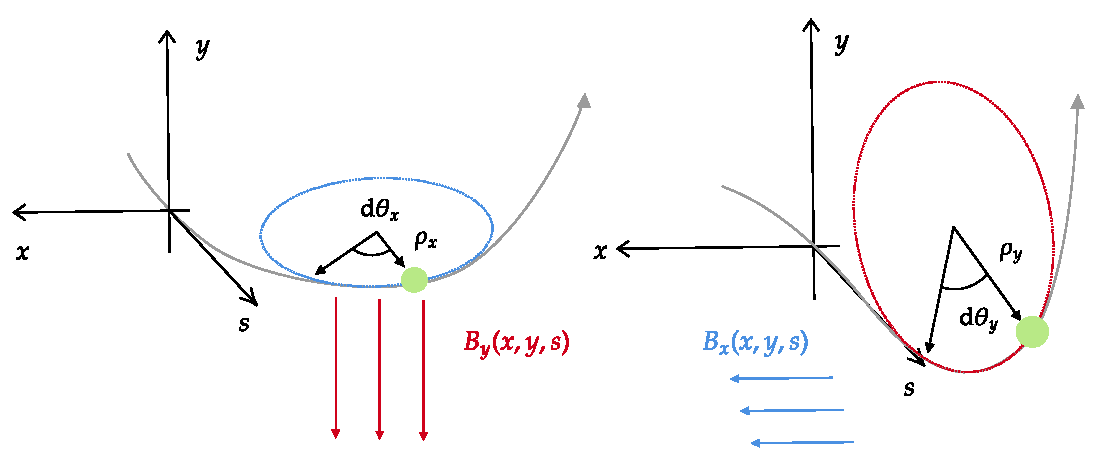
\includegraphics[width=\textwidth]{Images/deflections.pdf}
    \caption[Illustration of trajectory deflection when interacting with magnetic fields.]{Illustration of trajectory deflection when interacting with magnetic fields.}
    \label{fig:deflec_angles}
\end{figure}
Consider an electron traveling along a curve parameterized by the arc-length $s$ with respect to an arbitrary reference point. Define the normal and bi-normal unit vectors so that we can identify a $x-y$ plane perpendicular to the motion.  Let $B_x(x,y,s)$  and $B_y(x,y,s)$, denote the magnetic field components along the unit vectors. The interaction with the fields results in deflections of the trajectory, whose deflection angles $\dd\theta_u$ in the $u=x,y$ plane can be estimated from the local curvature radius $\rho_u$ and infinitesimal displacement $\dd{s}$ with the aid of a local, instantaneous version of equation~\eqref{eq:Lorentz}:
    \begin{equation}
        \begin{aligned}
            \dd{\theta_u} & = \frac{\dd{s}}{\rho_u(s)} = \frac{e}{p}B_v(x,y,s)\dd s = \frac{1}{R(p)}B_v(x,y,s)\dd s, \quad u,v=x, y \quad\text{or}\quad y,x.
        \end{aligned}
        \label{eq:deflec_angles}
    \end{equation}
Where eq.~\eqref{eq:rigidity} has been used to identify the $p/e$ ratio as the magnetic rigidity $R(p)$. These considerations are illustrated in Fig.~\ref{fig:deflec_angles}. The rigidity depends solely on the electron's momentum/energy and serves as the appropriate normalization constant to evaluate the instantaneous angular deflections in the electron's trajectory caused by magnetic fields.
\section{The coordinate system for storage ring dynamics}
As sketched by Fig.~\ref{fig:storage_ring}, electrons in a storage ring perform oscillations close to a nearly circular reference closed orbit. A convenient coordinate frame to describe the dynamics in this scenario can be constructed by imagining a reference particle traveling along a curve drawn by the tip of a vector $\vb{r}_0$, as Fig.~\ref{fig:frenet-serret} shows. This particle samples exactly the reference nominal orbit and travels a distance $s$ along the ring, which can be used to parameterize the motion. The triad of direction vectors for the co-moving coordinate frame consists of the vector $\vu{s}$, tangent to the trajectory, the vector $\vu{x}$, normal to the trajectory, pointing in the direction at which $\vu{s}$ changes, and a vector $\vu{y}=\vu{x}\cross\vu{s}$, bi-normal to the trajectory. This construction leads to a Frenet-Serret reference frame.

Assuming no curvature in the $y$ plane, i.e. that the accelerator defines a curve whose plane is parallel to the facility flat floor, then the tangent, normal and binormal unit vectors defining the frame can be calculated as \cite{lee_accelerator_2004}
\begin{equation}
\vu{s}=\dv{\vb{r}_{0}}{s}, \quad \vu{x}=-\rho\dv{\vu{s}}{s}, \quad \vu{y} =  \vu{x}\times\vu{s},
\end{equation}
where $\rho(s) = \norm{\dv*{\vu{s}}{s}}^{-1}$ is the local curvature radius\footnote{For a circular trajectory, $\vb{r}_0 = \mqty[R\cos(s/R) & R\sin(s/R) & 0]^\intercal$, $ 0\leq s \leq L$, in the laboratory frame. So we can calculate $\vu{s}=\mqty[-\sin(s/R) & \cos(s/R) & 0]^\intercal$, $\dv*{\vu{s}}{s} = -R^{-1}\mqty[\cos(s/R) & \sin(s/R) & 0]$, which reveals $\rho(s)=R$, justifying the interpretation of $\rho(s)$ as a curvature radius.}. The vectors evolve along $s$ as prescribed by the Frenet-Serret equations:
\begin{equation}
\dv{\vu{s}}{s}=-\frac{1}{\rho(s)}\vu{x}, \quad\dv{\vu{x}}{s}=\frac{1}{\rho(s)}\vu{s}, \quad \dv{\vu{y}}{s}=0.
\end{equation}
The frame depends solely on the geometry of the specified path: the instantaneous curvature $\rho^{-1}(s)$. Since the curvature is defined by the strengths of the dipolar fields $B_0(s)$ in the $y$ direction, then, eq.~\eqref{eq:deflec_angles} leads to
    \begin{equation}
        \frac{1}{\rho(s)} = \frac{B_0(s)}{R_0},
        \label{eq:G}
    \end{equation}
where $R_0$ is the rigidity of the beam at the nominal energy.
%As a starting point for designing the magnetic lattice of an accelerator, given the desired energy range for the beam and its rigidity and the desired radius of curvature, the required integrated strength of the dipoles must satisfy the above relation.

The transverse deviations from the nominal orbit can be measured as projections along the unit vectors $\vu{x}$, $\vu{y}$ in the normal and bi-normal directions. These deviations characterize the transverse dynamics of the electron. One may also be concerned with the distance of a given particle from the reference particle along the curve. Such differences arise due to differences in the energy of the two particles. In the full, six-dimensional dynamics, the longitudinal distance from the reference particle and the energy deviations are conjugate dynamical variables characterizing the longitudinal dynamics. They typically oscillate within a range of stable values, characterizing the energy acceptance. As mentioned above, since no radiation loss nor gain will be considered in our modeling, the energy and longitudinal deviations from the reference particle shall be static and treated as fixed parameters.

\begin{figure}[htb]
    \centering
    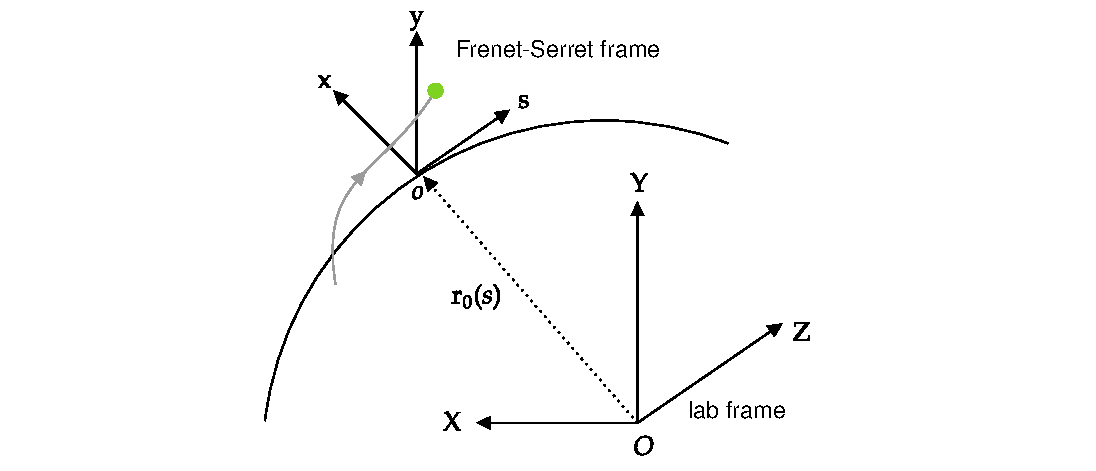
\includegraphics[width=0.9\textwidth]{Images/frenetserret.pdf}
    \caption[The Frenet-Serret coordinate system]{The Frenet-Serret coordinate system. Figure inspired by ref.~\cite{huang_beam-based_2019}.}
    \label{fig:frenet-serret}
\end{figure}

\section{Hamiltonian for the relativistic electron}
To the derive equations of motion for the electron in a storage ring, the Lorentz equation in the Frenet-Serret frame could be further developed. However, a more formal, systematic and rigorous derivation can be obtained via the canonical formalism. The dynamics of relativistic electrons influenced by electromagnetic fields $(\Phi, \vb{A})$ is encapsulated by the Hamiltonian \cite{landau_classical_1975}
    \begin{equation*}
        H=\sqrt{m^2c^4+(\vb{P}-e\vb{A})^2c^2}+e\Phi,
    \end{equation*}
 $e$ being the elementary charge and $\vb{P}=\vb{p}+e\vb{A}$ the canonical momentum, with $\vb{A}$ being the vector potential describing the magnetostatic fields of the lattice, i.e. $\vb{B}=\curl \vb{A}$. To obtain equations of motion for electrons in the storage ring, one usually follows the steps below:
 \begin{itemize}
    \item A canonical transformation to change coordinates is applied in order to describe the motion in terms of the Frenet-Serret frame variables $x$, $y$;
    \item Instead of time $t$, the Hamiltonian and the dynamical variables are described as functions of $s$, the longitudinal position along the ring;
    \item Paraxial approximation: the transverse momenta are assumed to be way smaller than the momentum along the trajectory's tangent direction. This allows the expansion of the square-root in the Hamiltonian as a power series, revealing the expression for an approximate Hamiltonian, which can be more easily handled;
    \item Geometric quantities are used: in the paraxial approximation, the canonical momenta for on-energy particles are identified with the derivatives with respect to the parameter $s$, i.e., $p_x = x^\prime = \dv*{x}{s}$ and $p_y = y^\prime = \dv*{y}{s}$, which represent the divergence angles from the nominal orbit. For off-energy particles, a correction factor is present;
 \end{itemize}
 All of the transformations and manipulations summarized above can be found in detail in the literature, such as in Refs.~\cite{lee_accelerator_2004, wiedemann_particle_2015,  wolski_beam_2014}. As mentioned previously, by neglecting RF cavities ($\Phi=0$) and radiation losses, the energy will be a constant parameter, and the dynamics will consist solely of the transverse degrees of freedom.  In this 4-dimensional dynamics, the set of canonical variables are $(x,p_{x},y , p_{y})$, where the momenta are given by
\begin{equation} p_{x}= x^\prime(1+\delta),\quad p_{y}=y^\prime (1+\delta)\end{equation}
and $\delta$ is the relative deviation from the nominal energy-momentum:
\begin{equation}
    \delta \equiv \frac{P-P_{0}}{P_{0}}\approx\frac{E-E_0}{E_0}.
\end{equation}
The ultra-relativistic approximation $E\approx pc$ was used. For on-energy particles, $p_x = x^\prime$, $p_y = y^\prime$.

Hamilton's equations for the paraxial-approximated Hamiltonian reveals the equations of motion for the $x$ and $y$ coordinates, which read:
\begin{equation}
x^{\prime \prime}=-\frac{(1+G x)^{2}}{1+\delta} \frac{B_{y}}{R_0}+G(1+G x),
\quad
y^{\prime \prime}=\frac{(1+G x)^{2}}{1+\delta} \frac{B_{x}}{R_0},
\label{eq:EOMs}
\end{equation}
where $R_0 = p_0/e$ is the magnetic rigidity of the beam at the nominal energy and $G(s)\equiv\rho^{-1}(s)$ is the inverse local radius of curvature, related to the dipole fields as in Eq.~\eqref{eq:G}.

\section{The magnetic fields}
To study the motion, we need to specify the fields $B_x(s)$ and $B_y(s)$ acting on the beam. Since in a storage ring the magnets are arranged as periodic arrays of dipoles, quadrupole, and sextupoles, the $B_x(s)$ and $B_y(s)$ functions are periodic. The magnetic fields are sectionally defined and have the following functional forms
\begin{itemize}
    \item Horizontal Dipole
           \begin{equation} B_x(s) = 0, \quad B_y(s) = B_0, \quad \text{inside dipoles},
            \label{eq:dipole}
           \end{equation}
    \item Normal quadrupole
          \begin{equation}B_x = B_1 y, \quad B_y = B_1 x, \quad \quad \text{inside quadrupoles},
            \label{eq:quadrupole}
           \end{equation}
    \item Normal sextupole
          \begin{equation}B_x = B_2xy, \quad B_y = \frac{1}{2}B_2(x^2 - y^2), \quad \quad \text{inside sextupoles},
            \label{eq:sextupole}
           \end{equation}
\end{itemize}
and zero everywhere else, in drift sections. Fields \eqref{eq:dipole}--\eqref{eq:sextupole}  are the so-called \textit{normal multipole fields}, in contrast with \textit{skew multipole fields}, which couple the horizontal and vertical dynamics. We will neglect skew fields and coupling for now. They can be treated as perturbations in perturbation theory schemes.

In eqs.~\eqref{eq:EOMs}, the magnetic rigidity normalizes all the fields. Thus, we define the normalized dipolar, quadrupolar and sextupolar field strengths, $G(s), K(s), S(s)$:
\begin{equation}
    G(s) = \frac{B_0(s)}{R_0}, \quad K(s) = \frac{B_1(s)}{R_0}, \quad S(s) = \frac{B_2(s)}{R_0}.
    \label{eq:mag_funcs}
\end{equation}
For a SIRIUS superperiod, the functions are shown in Fig.~\ref{fig:field_funcs}. A superperiod consists of the basic repetition of four magnetic cells. SIRIUS has 5 superperiods. In other words, the curves in Fig.~\ref{fig:field_funcs} repeat themselves five times along the $518~\unit{m}$ of the ring. More details on the magnetic lattice are in section~\ref{sec:mag_latt}.
\begin{figure}[htb]
    \centering
    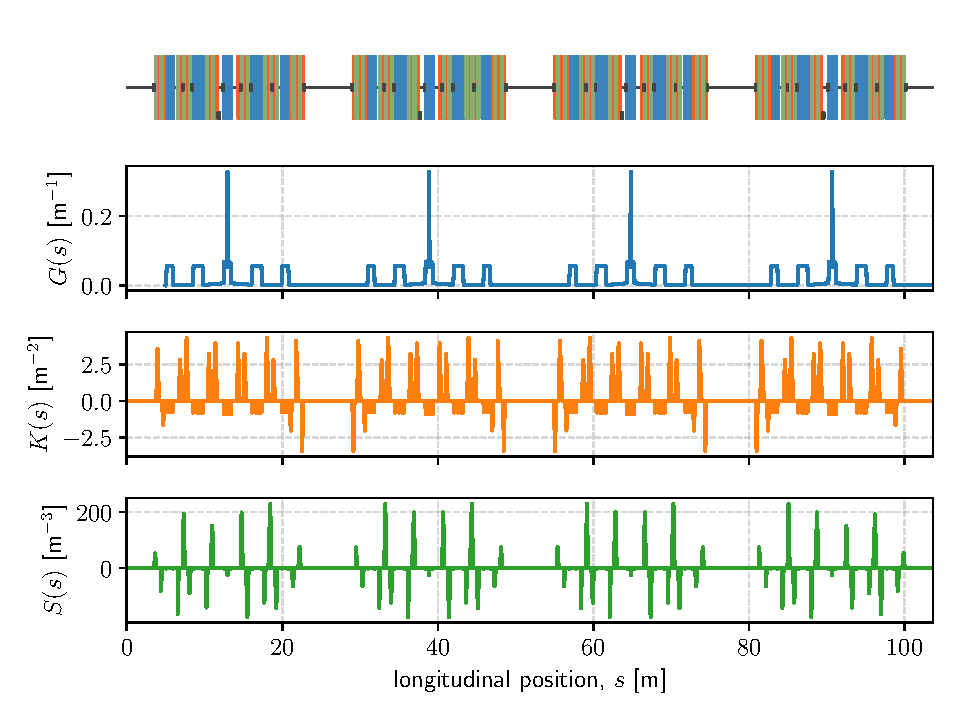
\includegraphics[width=\textwidth]{Images/field_functions.pdf}
    \caption[Normalized field functions for dipoles, quadrupoles and sextupoles of a superperiod of SIRIUS lattice]{Normalized field functions for dipoles (top plot), quadrupoles (middle plot) and sextupoles (bottom plot) of a superperiod of SIRIUS lattice, shown at the top. Colored blocks represent the magnets of the accelerator lattice: blue for dipoles, orange for quadrupoles and green for sextupoles. The ring has a 5-fold symmetry, with the cells, fields, and optics function repeating the pattern shown above five times up to $s=518~\unit{m}$.}
    \label{fig:field_funcs}
\end{figure}
\section{Linear dynamics}
Expansion of eqs.~\eqref{eq:EOMs} up to first order in the $x, y, \delta$ variables leads to \cite{sands_physics_1969}
    \begin{equation}
        x^{\prime\prime}+(G^2+K)x=G\delta, \quad
        y^{\prime\prime}-Ky=0.
        \label{eq:linearEOM}
    \end{equation}
    For on-momentum particles, $\delta=0$, both equations are instances of Hill's equations
    \begin{equation}
        u^{\prime\prime}+K_u(s)u = 0,
        \label{eq:Hill}
    \end{equation}
   i.e, a pair of parametric oscillators for $u=x,y$, with $s$-dependent and periodic focusing functions
         $$K_x(s) = G^2(s) + K(s), \quad K_y(s) = - K(s),$$
    the analogs to an oscillator's spring force per unit mass. Motion in the linear approximation thus consists of oscillations around the closed orbit, known as \textit{betatron oscillations}.
\subsection{Pseudoharmonic description}
Betatron motion can be cast in an amplitude-phase form. One can show that
\begin{equation}
    u(s) = \sqrt{2\beta_u(s) J_u}\cos(\phi_u(s) + \phi_0),\quad u=x,y,
    \label{eq:pseudo_harmon}
\end{equation}
is a solution to \eqref{eq:Hill}, as long as the $\beta_u(s)$ function satisfies the boundary-value problem
\begin{equation}
    \frac{1}{2}\beta_{u}^{\prime\prime}+\beta_{u} K_u(s) - \frac{1}{\beta_{u}}\qty(\frac{1}{4}\beta_{u}^{\prime 2} + 1 ) = 0, \quad
        \begin{cases}
            \beta_{u}(0) = \beta_{u}(L)\\ \beta_{u}^{\prime}(0) = \beta_{u}^{\prime}(L)
        \end{cases}
    \label{eq:beta_eq}
\end{equation}
and the phase advance is given by
    \begin{equation}
        \phi_u(s) = \int_{0}^{s}\frac{1}{\beta_u(\sigma)}\dd\sigma.
   \end{equation}
The motion is oscillatory, non-harmonic, and non-periodic. The oscillations envelope is the square-root of the beta functions $\beta_u(s)$, which for the SIRIUS storage ring are shown in Fig.~\ref{betafunc}.
\begin{figure}[htb]
    \centering
    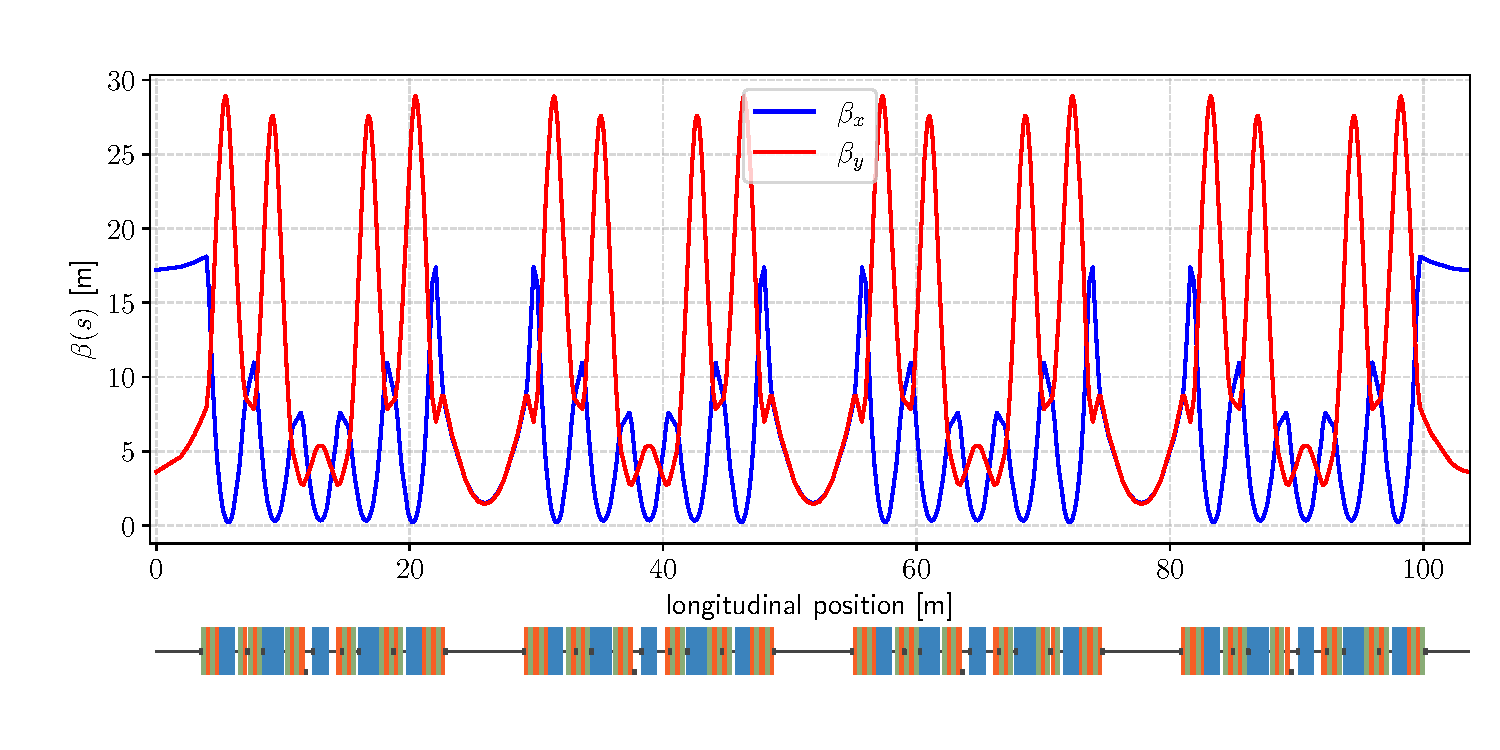
\includegraphics[width=\textwidth]{Images/beta_functions.pdf}
    \caption[Betatron functions in a superperiod of the SIRIUS storage ring]{Betatron functions in a superperiod of the SIRIUS storage ring.}
    \label{betafunc}
\end{figure}
\subsection{The tune}
An important parameter of the dynamics is the \textit{tune}: the phase advance over a revolution along the ring, in units of a complete cycle:
\begin{equation*}
    \nu_u=\frac{1}{2\pi}\int_{s}^{s+L}\frac{\dd \sigma}{\beta_u(\sigma)}\equiv\frac{1}{2\pi}\oint\frac{\dd s}{\beta_u(s)}.
\end{equation*}
The tune reveals the number of transverse oscillations per revolution along the ring. The optimized tunes during design phase for SIRIUS storage ring are $(\nu_x, \nu_y)=(49.08, 14.14)$. These were the machine tunes prior to this work.

When studying the effects of perturbations and nonlinearities acting on the beam, one realizes that tunes are global parameters in determining the beam's response. More specifically, the tunes impact over disturbances amplification factors, which are greatest when tunes are close to integer numbers. Ideally, it is desired for the tunes to be far from the integers, but also far from the half-integers. We examine the relation between the tunes and the effects of disturbances in more detail in section \ref{sec:field_err}.

\subsection{Turn-by-turn motion}
If one keeps track of the time evolution of the $u, u^\prime$ variables at a fixed position along the ring, plotting them in a phase space, one realizes the quasi-periodic motion traces out ellipses. This fact can be analytically verified by calculating the derivative
    \begin{equation}
        u^{\prime}(s) = - \sqrt{\frac{2J_u}{\beta_u}}\qty[\sin(\phi_u(s) + \phi_0) - \frac{1}{2}\beta_u^\prime(s)\cos(\phi_u(s) + \phi_0)],
        \label{eq:uprime}
    \end{equation}
    defining the functions $\alpha_u = -\frac{\beta_u^\prime}{2}$  and $\gamma_u = \frac{(1+\alpha_u^2)}{\beta_u}$ and checking that $u, u^\prime$ satisfy the quadratic form
    \begin{equation}
        2J_u=\gamma_u u^{2}+2\alpha_u u u^{\prime}+\beta_u u^{\prime2},
     \end{equation}
which describes the ellipse. The ellipse properties are determined by the $\beta_u(s), \alpha_u(s)$ and $\gamma_u(s)$ functions, also known as Courant-Snyder (C-S) parameters or Twiss parameters, as Fig.~\ref{fig:ellipse} shows. Since the parameters are functions of the position $s$, then, at each point along the accelerator, the Poincaré Section $u, u^\prime$ displays a different ellipse. Although different in shape, their areas are proportional to $J_u$, an invariant quantity determined by the particle's initial condition. The ellipse areas are thus conserved along the ring \cite{lee_accelerator_2004,wiedemann_particle_2015}.

 Since the phase advance over a turn is $2\pi \nu+\phi_0$, the phase advance after the $j$-th turn is $2\pi\nu j+\phi_0$. Therefore,
 sampling the transverse motion at a fixed $s=s_0$ position reveals a harmonic displacement, which at the $j$-th turn reads
\begin{equation}
    u_j(s_0)=\sqrt{2\beta_u(s_0) J_u}\cos(2\pi\nu_u j+\phi_u(s_0)).
    \label{eq:TbT_motion}
\end{equation}
Knowledge of this formula allows the determination of the tunes (mod $2\pi$) from the observation of \gls*{tbt} motion of the beam. The time-series of positions can be fitted to eq.~\eqref{eq:TbT_motion} in the time domain, or the signal can be processed in the frequency domain for the identification of the harmonic corresponding to $\nu_u$.
% Time of flight during a complete turn is $L/c$ so, for the $j$th turn, $t_j=\frac{L}{c} j$. With a revolution frequency of $\omega_r=2\pi/(L/c)$, we see that $2\pi j= \omega_r t_j$. As a function of the time elapsed over the $j$ turns, the displacements reads
% \begin{equation}
%     x_j=\sqrt{2\beta_0J}\cos(\omega_r\nu t_j+\phi_0).
% \end{equation}
\begin{figure}[htb]
    \centering
    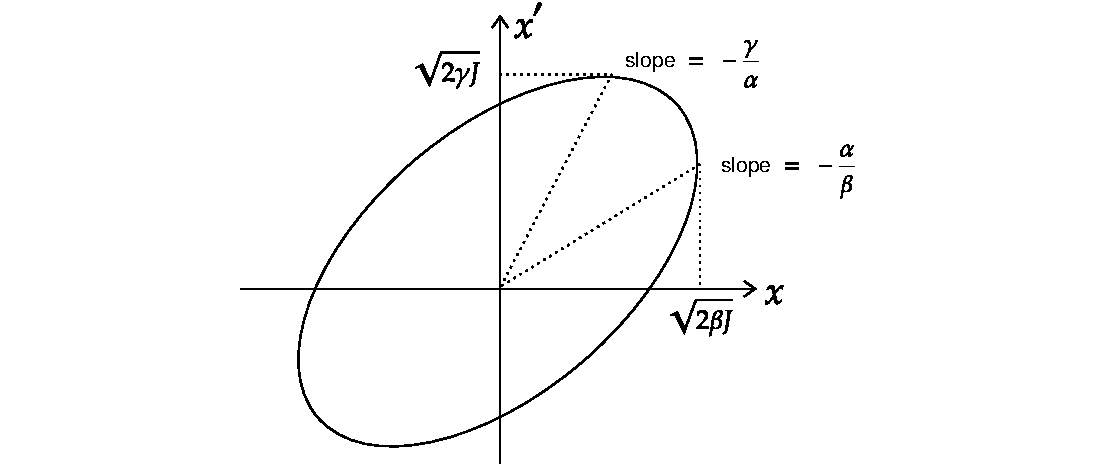
\includegraphics[width=0.9\textwidth]{Images/ellipse.pdf}
    \caption[Ellipse traced by TbT motion in the $(x,x^\prime)$ phase space.]{Ellipse traced by \gls*{tbt} motion in the $(x,x^\prime)$ phase space. Optics functions $\alpha(s), \beta(s), \gamma(s)$ determine the principal axes aspect-ratio and the ellipse inclination at each longitudinal position along the ring. Figure inspired by ref.~\cite{wolski_beam_2014}.}
    \label{fig:ellipse}
\end{figure}
\section{Dispersive \& chromatic effects and linear perturbations}
\subsection{Dispersion}
The equation of motion for off-momentum particles in the horizontal plane, the first of eqs.~\eqref{eq:linearEOM}, is a non-homogeneous Hill's equation. The solution consists of the linear combination of the homogeneous solution (betatron motion) and the particular solution: $x=x_\beta+ x_\delta$, which represents an additional deviation from the nominal orbit. Since the non-homogeneous term, $G(s)\delta$, is proportional to $\delta$, we can assume  $x_{\delta} = \eta(s)\delta$, where $\eta(s)$ is the \textit{dispersion function}. For this to be the solution, the dispersion should satisfy
    \begin{equation*}
        \eta^{\prime\prime}+(G^2+K)\eta=G,\quad
        \begin{cases}
            \eta(0) = \eta(L),\\
            \eta^\prime(0) = \eta^\prime(L).
        \end{cases}
    \end{equation*}
    The periodicity in the $\eta(s)$ function is required if we want to interpret it as a closed orbit distortion per relative momentum deviation. Thus, off-momentum particles perform betatron oscillations around a dispersive orbit, displaced from the nominal orbit by $\eta(s)\delta$. The dispersion function for the SIRIUS storage ring is shown in Fig.~\ref{dispersion_func}
    \begin{figure}[htb]
        \centering
        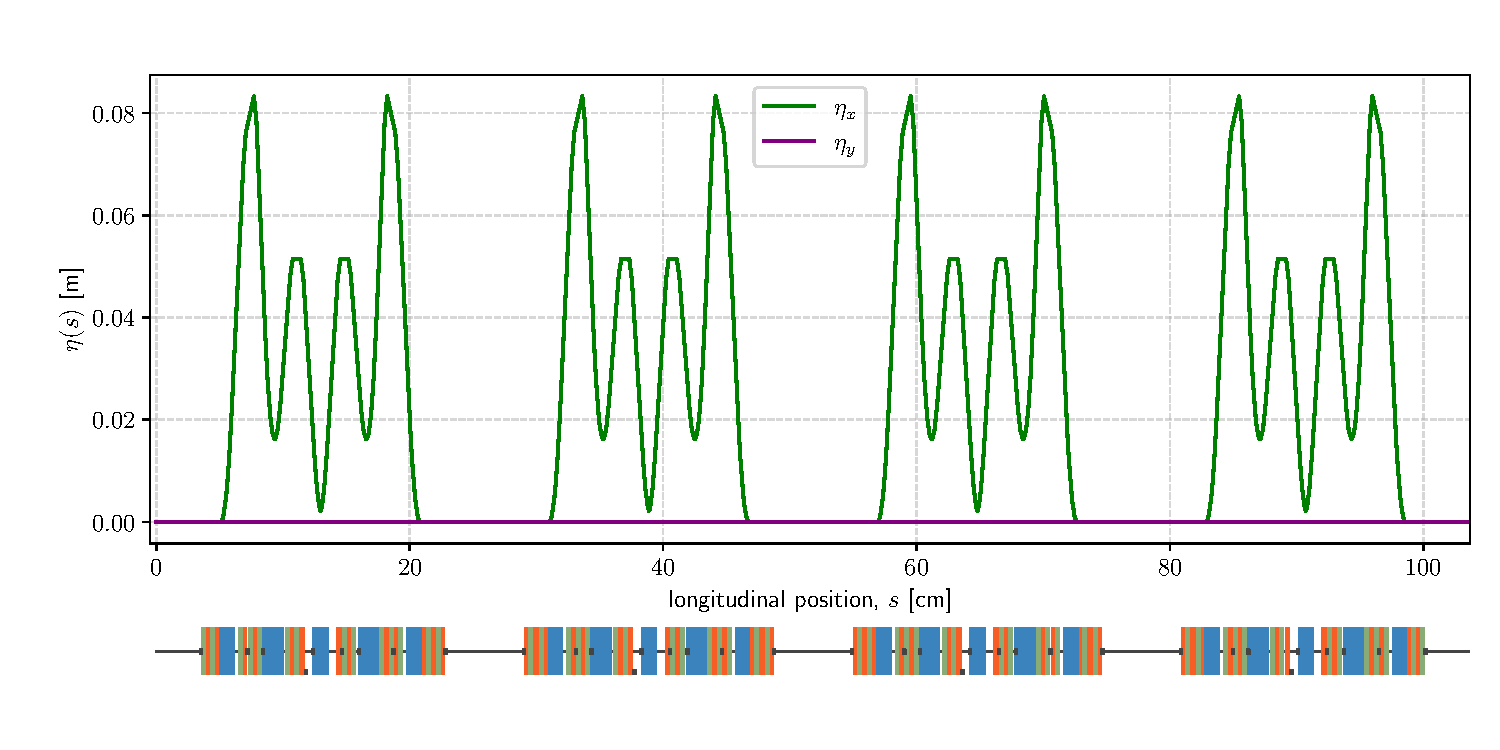
\includegraphics[width=\textwidth]{Images/dispersion.pdf}
        \caption[Dispersion function for a SIRIUS superperiod.]{Dispersion function for a SIRIUS superperiod.}
        \label{dispersion_func}
    \end{figure}
\subsection{Linear Field Errors}
\label{sec:field_err}
    % The dipolar contributions promote additional bendgin and thud disturb the design orbit. Assuming the perturbations are not strong enough to kill the beam, a distorted closed orbit must exist. To find it we need to find the coordinates along the ring which are mapped to themselves after a complete revolution. That is, we must find the fixed point $\vb{X}_{\text{co}}$ of the disturbed one-turn map:
    % \begin{equation}
    %     \vb{X}_{\text{co}} = \mathbf{M} \vb{X}_{\text{co}} + \boldsymbol{\Delta}
    % \end{equation}
    % where $\boldsymbol{\Delta} = (0, \theta)^\intercal$, $\theta = B_y \Delta s / B\rho$ for the $(x, x^\prime)$ slice of the closed orbit, $\theta = B_x \Delta s / B\rho$ for the $(y, y^\prime)$. Solving for the closed orbit we find
    % \begin{equation}
    %     \vb{X}_{\text{co}} = (\mathbf{I} - \mathbf{M})^{-1}\boldsymbol{\Delta}.
    % \end{equation}
    % Using the Courant-Snyder parametrization for the one-turn map at the point $s_0$ immediately downstream the perturbation leads to
    % \begin{equation}
    %     \vb{X}_\text{co} = \frac{\theta}{2\sin\pi\nu}\mqty(\beta_0 \cos\pi\nu \\ \sin\pi\nu - \alpha_0 \cos\pi\nu).
    % \end{equation}

In the presence of additional dipolar and quadrupolar fields representing field errors and deviations from the nominal fields, the orbit and focusing of the beam are changed. Assuming these are small perturbations and not sufficiently strong to perturb the beam severely, we can evaluate the disturbances to the unperturbed dynamics with a simple perturbation theory scheme. The details and derivations can be found in the literature, such as in chapter 2 of Ref. \cite{lee_accelerator_2004}. Here we highlight the main results.
\subsubsection{Dipole errors}
    Suppose there are additional dipole fields $\Delta B_{0x}(s), \Delta B_{0y}(s)$ interacting with the beam other than the dipole fields of the nominal lattice. These translate into errors of the dipolar functions: $\Delta G_y(s)=-\Delta B_{0x}(s)/R_0$ and $\Delta G_x(s)=\Delta B_{0y}(s)/R_0$. In this scenario, the equations of motion read
    \begin{equation}
        x^{\prime\prime}+K_x(s)x=G\delta + \Delta G_x(s), \quad
        y^{\prime\prime}+K_y(s)y = \Delta G_y(s).
        \label{eq:dip_errEOM}
    \end{equation}
    The solution consists of the combination of the betatron motion and the dispersive orbit (for the horizontal plane) plus the closed orbit distortion $u_{\text{co}}$ induced by the additional bending terms due to the dipole errors. For a single thin bending error $\Delta G_u$ in the $u=x,y$ plane, acting for a length $\Delta s$ around $s=s_0$, the closed orbit distortion $u_{\text{co}}$ reads
    \begin{equation}
        u_{\text{co}}(s) = \frac{\sqrt{\beta_u(s)\beta_u(s_0)}}{2\sin\pi\nu_u}\Delta G_u\cos( \pi\nu_u - |\phi_u(s)-\phi_u(s_0)|)\Delta s.
        \label{eq:cod}
    \end{equation}
    For a distribution $\Delta G_u(s)$ of dipolar perturbations along the ring, we sum over the contributions:
    \begin{equation}
        u_{\text{co}}(s) = \frac{\sqrt{\beta_u(s)}}{2\sin\pi\nu_u}\int_{s}^{s+L} \Delta G_u(\sigma)\sqrt{\beta_u(\sigma)}\cos(\pi\nu_u + \phi_u(s) - \phi_u(\sigma))\dd{\sigma}.
        \label{eq:co_dist}
    \end{equation}
    The prefactor involving the sine of the tune shows how $\nu_{u}$ close to an integer can amplify the effects of the dipolar perturbations on orbit distortions. At first, aiming for tunes half-integer tunes $\nu=k/2, k\in\mathbb{Z}$ might seem desirable to minimize the distortions. Choosing so, however, increases the sensitivity to gradient errors, which we examine next.
    % Knowledge of the beam-response to perturbations allows for the inversion of the problem. We can use specified small dipole kicks to correct the orbit, bringing it closer to the nominal one. These small dipole fields are generated by corrector magnets (CM's) abd orbit correction consists on linear problem of seeking CMs strength that minimze orbit distortions.

    % A quadrupole error can be represented by a thin-lens quadrupole transfer matrix \cite{Courant:1958wbj}
    % \begin{equation}
    %     \mathbf{M}_q = \mqty(1 & 0 \\ -k\Delta s & 1),
    %  \end{equation}
    %  so that, immediately downstream the error, the transfer matrix reads $\mathbf{M} = \mathbf{M}_q \mathbf{M}_0$. As a consequence, the optics deviates from the nominal optics. More notouriously, the beta and the phase advances, and thus tune, changes.

    %  The phase advance over a turn, $\phi$, is related to the trace of the one-turn transfer matrix $\mathbf{M}$ as $\cos\phi = 2 \tr \mathbf{M}$. Using the CS parametrization for $\mathbf{M}$, performing the multiplication $\mathbf{M}_q \mathbf{M}_0$ and calcualting the trace leads to
    %  \begin{equation}
    %     \cos \phi - \cos\phi_0 = - \frac{1}{2} k(s)\Delta s \beta_0 \sin\phi_0.
    %  \end{equation}
    %  In a linear approximation (if $\sin \phi_0$ is not near zero) $\Delta(\cos \phi) = \cos \phi - \cos\phi_0 \approx \Delta \phi\dv*{(\cos \phi)}{\phi}$ so the tune-shift due to a single thin-lens quadrupole error is
\subsubsection{Gradient errors}
Gradient errors can be modeled as corrections to the focusing functions in the equations of motion: $K_u(s)\to K_u(s) + \Delta K_u(s)$, for $\Delta K_x(s) = \Delta B_{1y}(s)/R_0$ and $\Delta K_y(s) = -\Delta B_{1x}(s)/R_0$. The changes in beam focusing lead to changes in the beta-functions, phase advances and, consequently, the betatron tunes. One can show the tune-shift as a consequence of a focusing gradient error $\Delta K_u$, acting during a small longitudinal extent $\Delta s$ around $s=s_0$ is \cite{lee_accelerator_2004}
\begin{equation}
    \Delta \nu_u = \frac{1}{4\pi} \beta(s_0) \Delta K_u \Delta s.
    \label{eq:delta_nu}
\end{equation}
Were we dealing with a defocusing error, a minus sign would preceed the above equation. For a distribution of errors we sum over the ring:
\begin{equation}
    \Delta \nu = \frac{1}{4\pi}\oint \beta(s) \Delta K(s) \dd s,
    \label{eq:delta_nu_dist}
\end{equation}
where the closed integration sign refers to a complete circulation along the ring, i.e., integration from $s_0$ to $s_0+L$, for any $s_0\in[0,L)$.

    %  Besides calculating the tune-shift, the resulting transfer-matrix for the lattice with errors allows for the identification of the new optics $\alpha, \beta, \gamma$, which can then be propagated to anywhere in the ring. In particular we can identify $\beta$ and its fractional deviation from the nominal value along $s$, a parameter known as \textit{beta-beating}
    As for the induced error on the beta-functions, it is possible to show that the relative error, known as beta-beat, can be expressed as
     \begin{equation}
        \frac{\Delta \beta_u(s)}{\beta_u(s)} = - \frac{1}{2\sin(2\pi\nu_u)}\int_{s}^{s+L}\beta(\sigma)\Delta K_u(\sigma)\cos[2(\phi_u(\sigma)-\phi_u(s)-\pi\nu)]\dd\sigma.
        \label{eq:beta_beat}
     \end{equation}
which is the largest for $2\nu_u$ closest to an integer. This means we must avoid tunes close to half-integers if we want to avoid the coherent build-up of betatron amplitudes, which can eventually lead to beam loss.
Integer or half-integer tunes are the simplest instances of resonances the beam can be subject to. A more general overview of resonances is presented in subsection~\ref{subsec:resons}.
% \begin{figure}
%     \centering
%     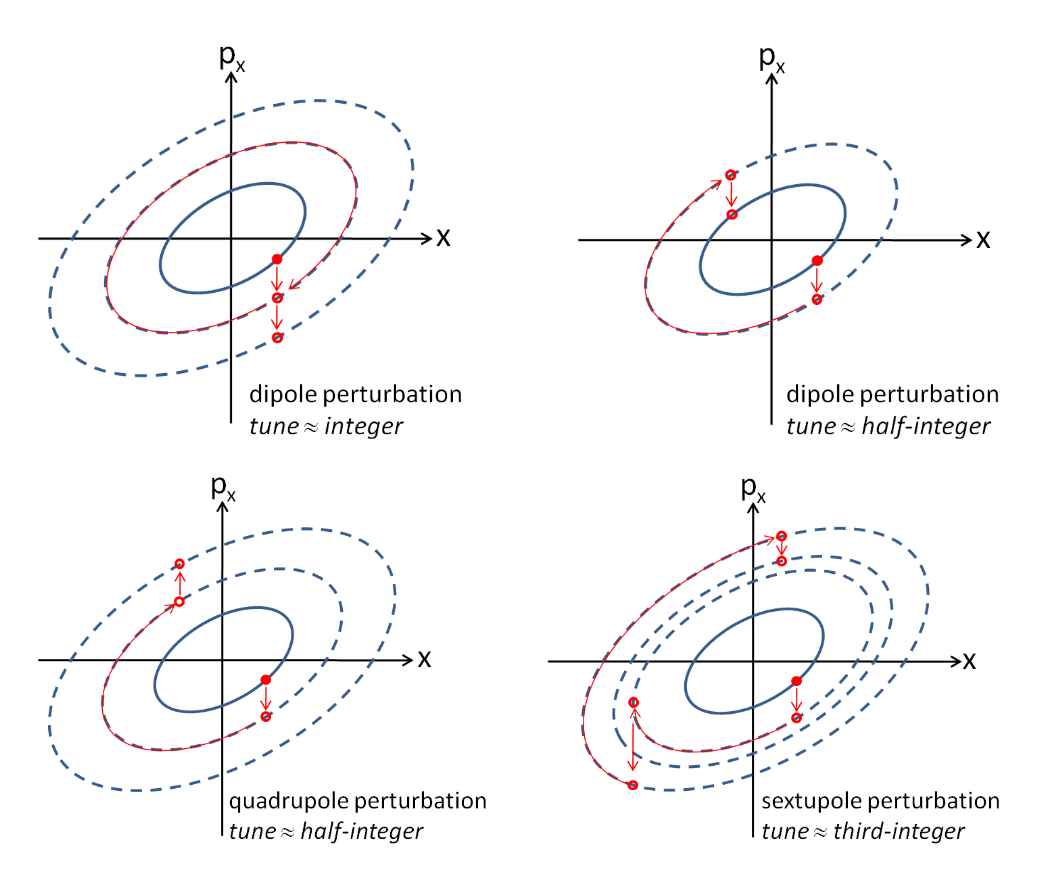
\includegraphics[width=0.6\textwidth]{Images/resonances.png}
%     \caption{!Redo fig: include only dipole and quadrupole! Illustration of phase-space motion under dipolar and quadrupolar perturbations close and away from resonances.}
% \end{figure}
\subsection{Chromaticity}
We have seen how the bending angles at the dipoles are different for electrons with different energies. This is the origin of dispersive orbits. However, energy deviations affect not only the closed orbit by means of the dispersion effect, but also the focusing of the trajectories, since a more/less energetic beam has higher/lower rigidity and thus is focused differently when passing through gradient fields.
%
% As for the higher order effect on the focusing, also known as chromatic effect, we consider the motion in a straight section under a gradient, so that there is no non-homogeneous term in the horizontal equation. The equation of motion considering $x\delta $ terms reads
% \begin{equation}
%     x^{\prime\prime}+(K_x+\Delta K_x)x=0
% \end{equation}
% \begin{equation}
%     y^{\prime\prime}+(K_y+\Delta K_y)y=0
% \end{equation}
% where $K_x=h^2+K_1$, e $K_y=-K_1$ and

Expansion of the equations of motion, eqs.~\eqref{eq:EOMs}, for off-energy particles up to the order of terms $u\delta$ (for $u=x,y$) reveals additional higher-order gradient errors. The focusing functions are corrected by $K_u(s)\to K_u(s) + \Delta K_u(s)$ \cite{lee_accelerator_2004,huang_beam-based_2019}, where
\begin{equation}
    \Delta K_x = -(K+2G^2)\delta \approx - K_x\delta
\end{equation}
\begin{equation}
    \Delta K_y = K\delta = - K_y\delta
\end{equation}
This means there exists an energy-dependent tune-shift effect caused by the gradient error. Using eq.~\eqref{eq:delta_nu_dist}, the tune-shift reads
% The result is that an off-momentum partcile sees a different optics along the ring: different beta function and different phase advance. Thus, it deviates from nominal operation conditions, specially in the tunes, inducing the tune-shifts
\begin{equation}
    \Delta \nu_u = - \frac{1}{4\pi}\oint\beta_u K_u \delta \dd{s},
    \label{eq:energy_delta_tune}
\end{equation}
for the $u=x,y$ planes. We can define the \textit{linear chromaticity} in the $u=x,y$ direction as tune-shift $\Delta \nu_u$ per relative energy deviation $\delta$:
\begin{equation}
    \xi_u=\dv{\nu_u}{\delta}.
\end{equation}
 The chromaticity created by the linear lattice is also called natural chromaticity. Using expression \eqref{eq:energy_delta_tune} for the tune-shift, the natural chromaticity reads
\begin{equation}
\xi_{u, \text {nat }} =-\frac{1}{4 \pi} \oint K_u \beta_u \dd{s}.
\end{equation}

This chromatic aberration effect needs to be corrected to guarantee energy-independent focusing. Correction can be attained with the insertion of sextupolar fields, specifically in the dispersive sections of the storage ring. In such regions, off-energy particles follow a dispersive orbit, and their position reads $x(s)=x_{\beta}(s)+\eta(s) \delta$, where $x_{\beta}(s)$ consists on the betatron oscillations. Since sextupolar fields are of the form
$$B_{x}=B_{2} x y, \quad B_{y}= \frac{B_{2}}{2}(x^{2}-y^{2}),$$
then, the off-momentum particles "see" the fields
$$B_{x}=B_{2}(x_\beta y + \eta \delta y), \quad B_{y}=\frac{B_{2}}{2}({x_\beta^{2}-y^{2}})+B_2 x_\beta \eta \delta + \frac{B_2}{2}(\eta \delta)^2.$$
So, to lowest order in eqs.~\eqref{eq:EOMs}, they feel a dipolar perturbation (which contributes to orbit distortions) and the following gradient perturbation:
$$\Delta K_{x,y}(\delta)=\pm S\eta \delta,$$
recalling that $S(s) = B_2 / R_0$.

Considering the contributions from both the errors induced by energy deviations and also the lowest order sextupole gradient effect, we have a  gradient shift of $\Delta K_u = -(K_u \mp S\eta)\delta$ to be inserted in eq.~\eqref{eq:delta_nu_dist}. The chromaticity in a lattice with sextupoles thus reads
\begin{equation}
    \xi_{u}=-\frac{1}{4\pi}\oint\beta_{u}(K_{u}\mp S\eta)\dd{s},
    \label{eq:chromaticity}
\end{equation}
with the minus sign for $u=x$ and the plus sign for $u=y$.

Formula~\eqref{eq:chromaticity} reveals that chromaticity depends linearly on sextupole strengths. This allows for its correction and tuning to desired values. In the SIRIUS storage ring, the operation chromaticity of about $+2.5$ for each plane was determined with the objective of mitigating the transverse instabilities induced by the resistive-wall effect in the range of currents the storage ring is expected to operate: $100$ to $350~\unit{mA}$ \cite[section 7.3]{sa_study_2018}.

 Since a focusing sextupole field focuses in a given plane and defocuses in the other, at least two sextupole families are required for chromaticity correction. To optimize the sextupole strengths required for correction, one family must be placed where $\beta_x > \beta_y$ and another where $\beta_y < \beta_x$. The cost of correcting chromaticity with sextupole is the insertion of nonlinearities in the dynamics. If on the one-hand, amplitude-dependent focusing is needed to correct the energy-dependent focusing (chromaticity), on the other hand it also influence particles with large amplitudes with nonlinearities. To allow for more control over the nonlinear effects and optimization of the dynamics, some families of sextupoles are also placed in non-dispersive sections. They are called achromatic families, since they have no effect over chromaticity up to leading order.
\begin{figure}
    \centering
    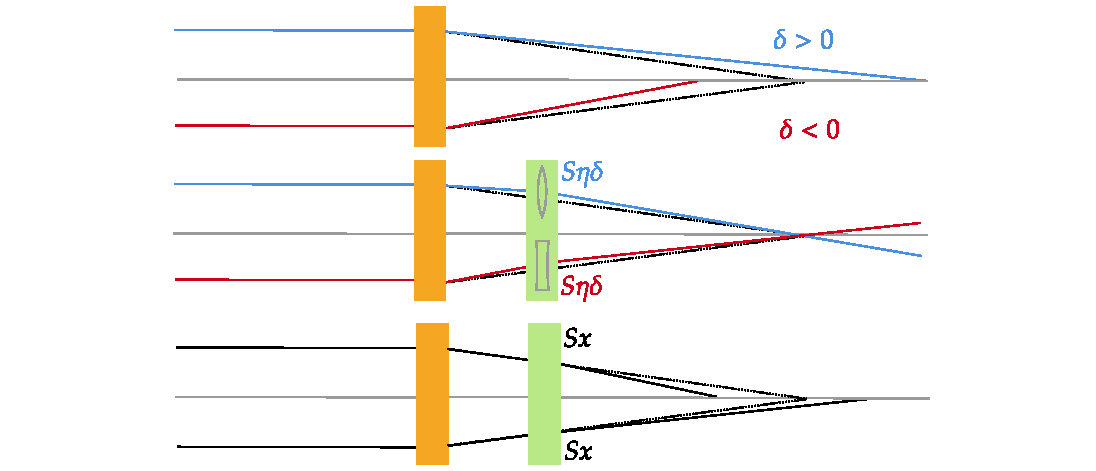
\includegraphics[width=\textwidth]{Images/chromaticity.pdf}
    \caption[Illustration of chromatic aberrations, their correction with sextupoles and examples of geometric aberrations.]{Illustration of chromatic aberrations (top), their correction with sextupoles (middle) and examples of geometric aberrations (bottom).}
    \label{fig:chromaticity}
\end{figure}

\section{Nonlinear dynamics, perturbations, resonances and tune-shifts}
The fields of sextupoles make the dynamics intrinsically nonlinear. To understand the effects of nonlinearities in a generic manner, we develop a basic Hamiltonian perturbation theory in the upcoming sections. However, this requires us to step back momentarily to review linear dynamics in the action-angle variables formalism, upon which we proceed with canonical perturbation theory.
\subsection{Action-Angle Variables}
The betatron equations of motion, Eqs.~\eqref{eq:Hill}, can be obtained as Hamilton's equations for an effective, linear Hamiltonian
\begin{equation}
    \mathcal{H}_u=\frac{1}{2}u^{\prime2}+\frac{1}{2}K_u(s)u^2,
\end{equation}
summed over $u=x,y$.
A transformation $(u,u^\prime)\to(\psi_u, J_u)$ to Action-angle variables is implicitly implemented by the type--1 generating function \cite{lee_accelerator_2004}
\begin{equation}
    F_1(u,\phi_u)=\int{u}^\prime\dd{{u}}=-\frac{u^2}{2\beta_u}\qty(\tan \phi_u-\frac{\beta_u^\prime}{2}).
\end{equation}
The action variable reads
\begin{equation}
    J_u=-\pdv{F_1}{\phi_u} = \frac{u^2}{2\beta_u}\sec^2\phi_u = \frac{1}{2\beta_u}[u^2 + (\beta_u u^\prime + \alpha_u u^2)],
    \label{eq:action}
\end{equation}
from which we can recover the pseudo-harmonic form $u=\sqrt{2\beta_u J_u}\cos(\phi_u(s)+\phi_0)$, and identify the constant $J$ we met before as the action and the betatron phase advance as the angle variable.

In the $J,\phi$ variables, the new Hamiltonian is $H_0(\phi, J)$,  given by
\begin{equation}
    H_u=\mathcal{H}_u+\pdv{F_1}{s} = \frac{J_u}{\beta_u}.
\end{equation}
Performing the change to action-angle variables in both the horizontal and vertical planes, we find the action-angle Hamiltonian for 4D dynamics:
\begin{equation}
    H_0= \frac{J_x}{\beta_x} +  \frac{J_y}{\beta_y}.
\end{equation}
Hamilton's equations read
\begin{equation}
    \phi_u^\prime = \frac{1}{\beta_u(s)},\qquad J_u^\prime=0.
\end{equation}
\subsection{Perturbations and tune-shifts}
Linear motion is integrable since it can be written in terms of the action variable only (angle-independent Hamiltonian). This means the action variable is a constant of motion.

Linear motion, though, is only a useful first approximation. In reality, in a storage ring, there are higher-order multipole magnets, such as sextupole magnets, and also multipole, alignment and excitation errors acting as perturbations. Generically referring to perturbations as the potential $V(J, \phi)$, we can write the perturbed Hamiltonian
\begin{equation}
    H(J,\phi) =H_0 + V(J,\phi),
\end{equation}
For which Hamilton's equations read
\begin{equation}
\phi_u^\prime = \frac{1}{\beta_u(s)}+\pdv{V(J,\phi)}{J_u}, \quad J_u^\prime = -\pdv{V(J,\phi)}{\phi_u}.
\end{equation}
The action is no longer an invariant. It changes as prescribed by the rate of change of the potential with respect to the phase. The phase also changes. The phase advance rate deviates from the linear betatron phase advance, which translates directly into tune-shifts. In this scenario, the tunes depend not only on the momentum, via the chromaticity, but also on the amplitudes (actions). In a general form, we can be express the tunes as
\begin{equation}
    \nu_u = \nu_{u0} + \xi_u(\delta) \delta + \alpha_{uu} J_u + \alpha_{uv} J_v,
\end{equation}
where $\xi_u$ represents the energy-dependent tune-shifts (higher-order generalization of the linear chromaticity), and the other components consist on the amplitude-dependent tune-shifts, up to first order in the actions.
\begin{figure}
    \centering
    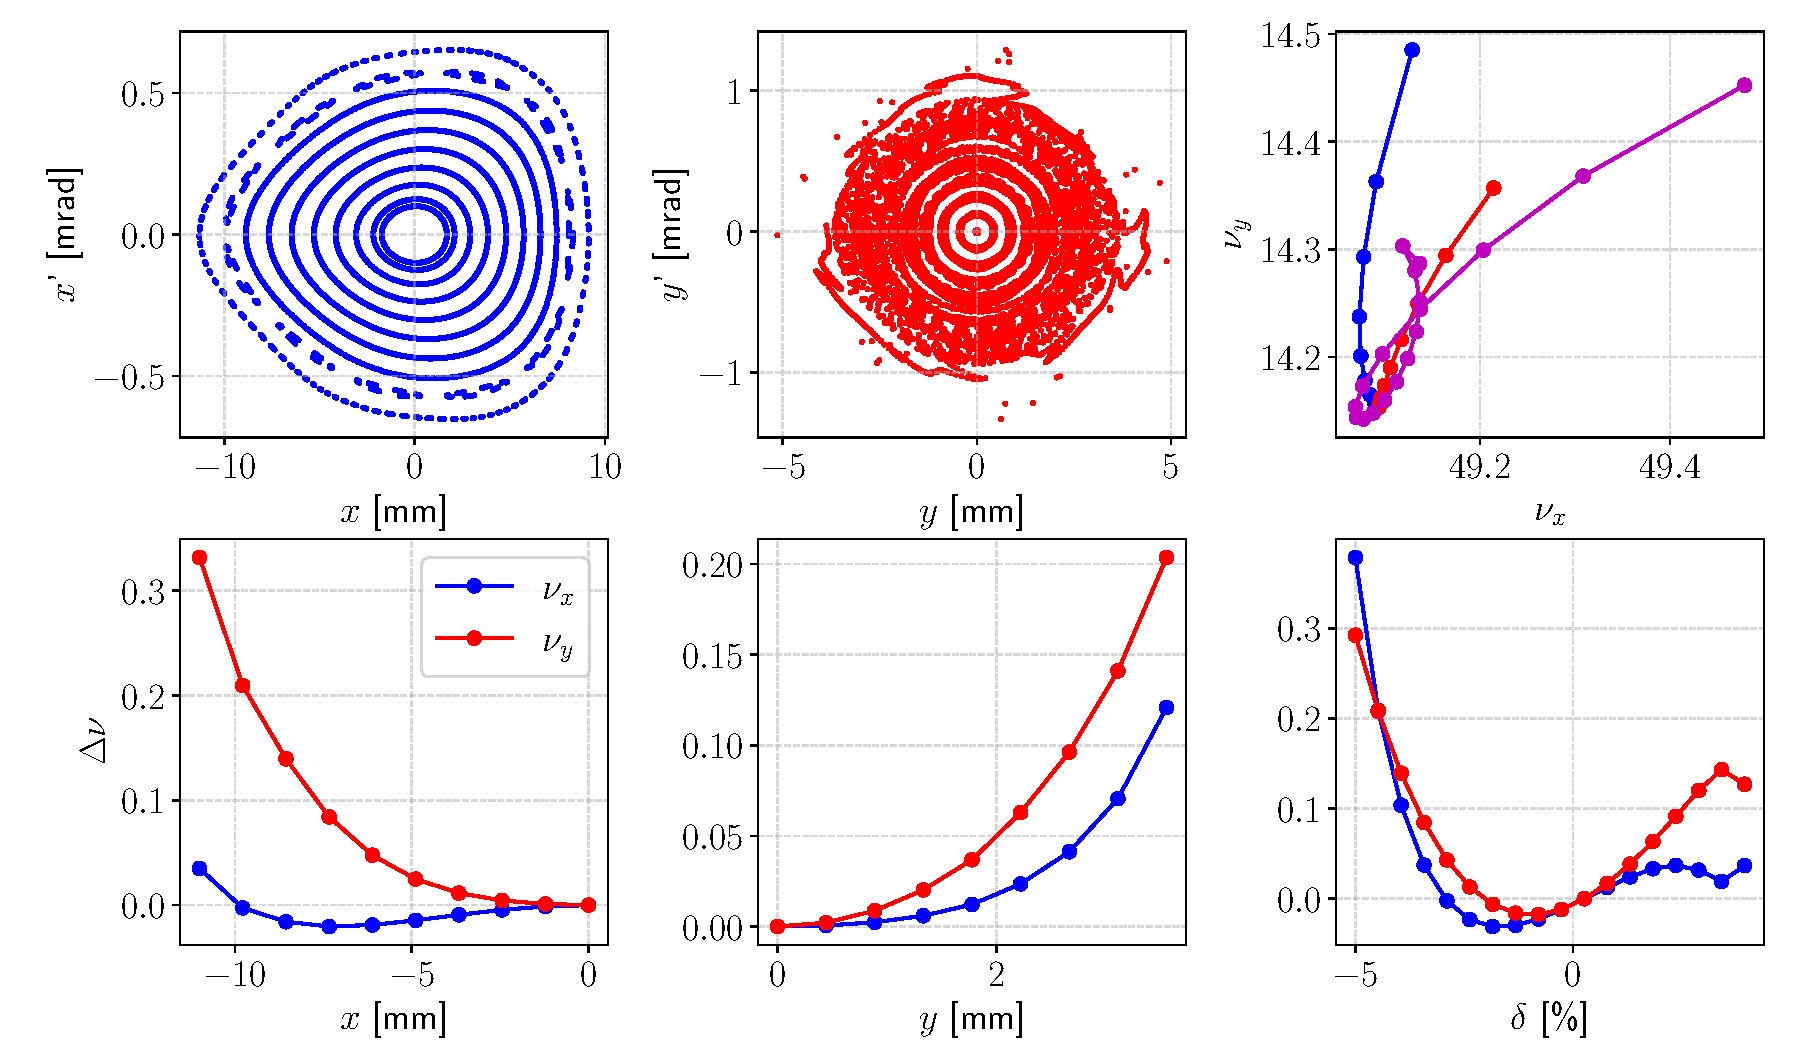
\includegraphics[width=\textwidth]{Images/nonlinear_dynamics_phase_tunes.pdf}
    \caption[Illustration of main characteristics in nonlinear dynamics]{Illustration of main characteristics in nonlinear dynamics. a) \& b): Poincaré sections for motion with increasing horizontal \& vertical amplitudes, respectively; c) Path traced in tune-space for each ellipse of a) in blue, for b) in red, and for each $\delta$ in f), in purple. d) \& e): $x$ and $y$ amplitude-dependent tune-shifts for each ellipse of a) \& b), respectively; f) energy-dependent tune-shifts}
    \label{fig:tune_shifts}
\end{figure}

Figure~\ref{fig:tune_shifts} highlights the main characteristics of the nonlinear dynamics. In a) and b) particles are simulated in SIRIUS' computer model with increasingly larger initial amplitudes in the $x$ and $y$ planes, respectively. The large-amplitude ellipses are distorted, since the action $J$ is no longer an integral of motion. Some large-amplitude particles do not survive. In d) and e), the deviations in horizontal and vertical tunes are shown for the a) and b) simulations, respectively. In d), the tune-shifts in the $y$ and $x$ planes are shown for each initial $x$ amplitude. In e), the tune-shifts for each initial $y$ amplitude in b) is shown. These plots outline the distortion of phase space ellipses, the existence of limiting amplitudes under which regular motion occurs, and the dependence of the tunes with the amplitudes.

In plot e) of Fig.~\ref{fig:tune_shifts}, the chromatic (energy-dependent) tune-shifts are shown: the tune-shifts of particle simulated with energy deviations in the range of $-5\%$ to $5\%$. Linear chromaticity is the derivative of this curve around $\delta=0$. In c), the blue curve represents the path traced in tune-space as the $x$ amplitude increase, i.e., the tunes for each initial condition of the simulations in a); the red curve represents the path traced as the $y$ amplitudes increase,  i.e., the tunes for each initial condition of the simulations in b). The purple curve is the path traced for each $\delta$ in the simulations shown at f).
\subsection{Resonances}
\label{subsec:resons}

4D linear unperturbed motion consists of the motion of two uncoupled parametric oscillators. As a quasi-periodic integrable system, the phase-space is diffeomorphic to the 2-Torus, $\mathbb{T}^2$, and there are an infinite number of such tori covering phase space, corresponding to the different choices of initial conditions $J_u$.

Canonical perturbation theory applied to perturbed motion fails to converge whenever the ratio of tunes is sufficiently rational (resonant tori). The Poincare-Birkhoff theorem states that under such conditions, almost all the periodic phase-space orbits disappear, i.e., almost all the tori are destroyed. An even number of tori survive, half stable and half unstable \cite[section 10.2]{marcus_mecanica2023}. Unstable motion in a storage ring eventually leads to beam loss.

The condition for sufficiently rational tunes, i.e, resonant tori, can be expressed as
\begin{equation}
        m\nu_x + n\nu_y = \ell,
        \label{eq:resonance_condition}
\end{equation}
    for $n, m, \ell\in\mathbb{Z}$. This condition defines lines in tune-space corresponding to the locus in which perturbation theory fails and motion can become unstable: resonance lines.

    We say $|n|+|m|$ is the order of the resonance, which is related to the order of the multipole field perturbation from which it arises.
    %  e.g: order 1 resonances can be driven by dipolar fields, as well as quadrupolar and sextupolar gradients; order 2 can be driven by quadrupolar and sextupolar components; and order 3 can be driven by sextupolar fields.
    Resonances arising from linear field errors, already anticipated in section~\ref{sec:field_err}, are those described by $\nu_x=\ell$ or $\nu_y =\ell, \ell\in\mathbb{Z}$. Normal gradient field errors drive $2\nu_x=\ell$ or $2\nu_y =\ell$ resonances. Skew gradients couple both planes and can drive the famous sum and difference resonances $\nu_x + \nu_y = \ell, \nu_x - \nu_y = \ell$. Sextupoles, up to first-order in perturbation theory, can drive the $3\nu_x=\ell$, resonance, as well as $\nu_x \pm 2\nu_y = \ell$ and $\nu_x =\ell$ resonances \cite[section 11.2.4]{wolski_beam_2014}. Figure~\ref{fig:resons} depicts resonance lines in tune-space for resonances up to second, third and fourth order, in the left, middle and right plots, respectively.
\begin{figure}[thb]
    \centering
    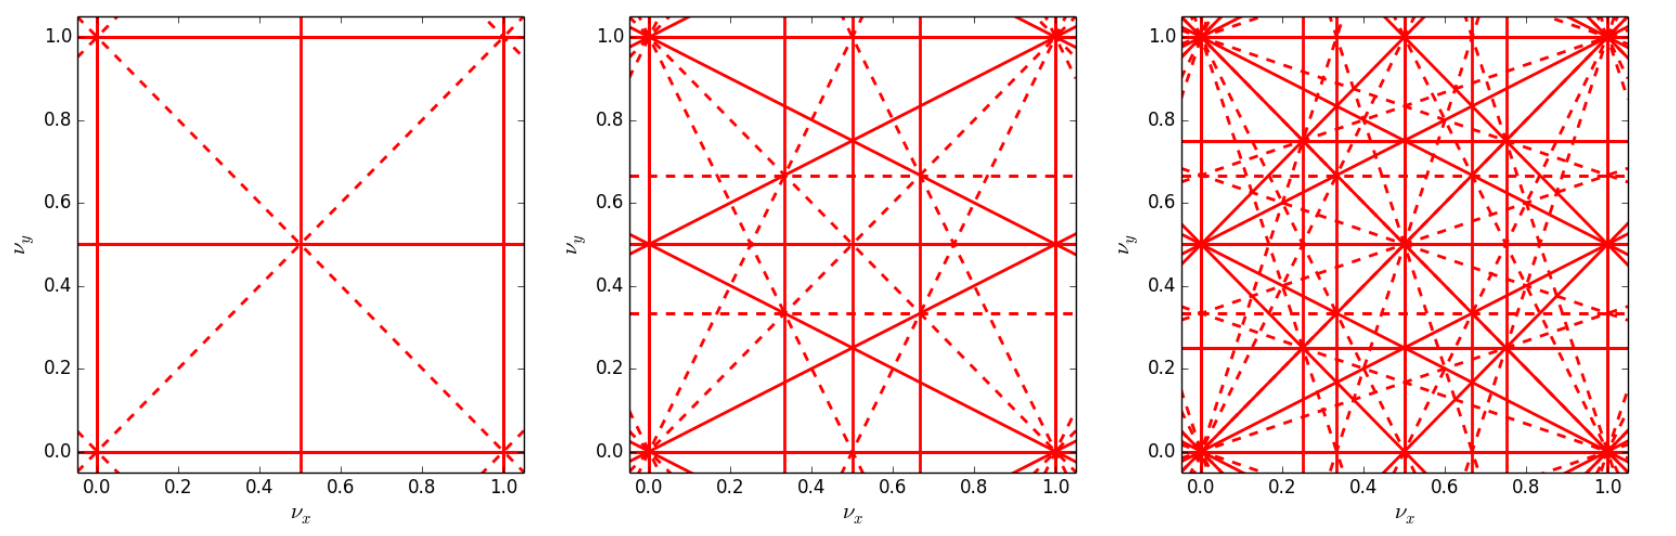
\includegraphics[width=\textwidth]{Images/tunes.png}
    \caption[Resonance lines in tune space up to 2nd, 3rd and 4th order.]{Resonance lines in tune space up to 2nd, 3rd and 4th order, respectively. Solid lines correspond to resonances driven by normal multipole fields, while dashed lines correspond to resonances driven by skew multipole fields. Figure adapted from ref.~\cite{bartosik_first2022}}
    \label{fig:resons}
\end{figure}
\subsection{The Dynamic Aperture}
    The stability of nonlinear dynamics can become sensitive when amplitudes are large. In this scenario, the effects of the nonlinear fields become more significant and the perturbations are dialed up, breaking down the stable tori. Even low-amplitude motion can be dangerous in the long-term due to the phenomenon of Arnold diffusion \cite{wolski_beam_2014, arnold_instability1964}: because of the tune-shifts, especially the amplitude-dependent tune shifts, the tunes can wander in tune space and eventually cross resonance conditions.

    Despite the complexity of predicting the stability of nonlinear perturbed dynamics theoretically, in electron storage rings, we usually observe the existence of an amplitude limit beyond which instabilities increase and the particles are lost, while the particles below the limiting amplitudes survive. In other words, there are limitations to the maximum transverse amplitudes displaying regular and bounded motion. This behavior was anticipated by the simulations shown in plots a) and b) of Fig.~\ref{fig:tune_shifts} and is also verified in the actual machine during experiments.

The border of the region of stability is the \textit{dynamic aperture} (\acrshort*{DA}). This term can be used to refer to the limiting amplitudes in any of the dynamical variables of phase-space. In this work, we are mostly concerned with the \gls*{DA} in the $(x, x^\prime)$ phase space because of its importance during the beam injection for accumulation into the storage ring.

During injection, if the horizontal amplitudes are larger than the \gls*{DA} along $x$ or $x^\prime$, the beam is not captured efficiently into the storage ring. In this case, increasing the \gls*{DA} to accommodate the incoming beam would be interesting, which is exactly what we aimed at while developing this project.

Since the \gls*{DA} is determined by the nonlinear perturbations, it is possible that tuning the nonlinear fields in a particular manner can render an optimum configuration with increased \gls*{DA}.  In the upcoming chapter, this idea is developed in more detail.

\chapter{Online Optimization}
This chapter defines, introduces and justifies online optimization  of synchrotron storage rings nonlinear dynamics. The Robust Conjugate Direction Search (RCDS) algor ithm is introduced, as well as the other optimization routines from which it was built upon. This chapter adds no novelty to the literature in optimization. It is an overview for merely pedagogic purposes. It mostly draws from the discussion presented by Numerical Recipes, ref.~\cite{press_numerical_2007}, as well as chapters 7 and 8 of ref.~\cite{huang_beam-based_2019} and ref.~\cite{huang_algorithm_2013}.
\section{Defining Online Optimization}
Consider a system that possesses some sort of figure of merit which depends on the collective state of a set of relevant components, parts, or operation modes which constitute the  parameters or decision variables. There is no mechanistic/deterministic or probabilistic model for the dependence of the figure of merit on the parameters' state, but it is well known that the parameters affect the figure of merit. One may call the relevant parameters knobs, since they can be used to tune the figure of merit.

Now suppose one wants to tune the knobs so the figure of merit reaches a certain value, or so that it is minimized or maximized. This is an optimization problem, with the figure of merit being the objective function. Since the whole system is a black-box, to measure different values for the objective function, i.e., to sample it, the knobs must be varied and the objective function must be measured, a process that may be expensive. The tuning procedure thus consists on trial-and-error iterations of changing the knobs, evaluating the objection and judging the quality of the changes performed.

A computer-automated routine or algorithm employing some strategy to seek the desired value or extremum of the objective function while the machine functioning is what we define as online optimization. The program must measure the objective function, read the current state of the knobs, calculate or decide and apply the changes to the knobs, measure the objective again and evaluate the quality of the changes over the objective. It incorporates this information when making the decision on how much to change the knobs next. The process is iterated until the desired outcome is reached.

The Dynamic Aperture (DA) optimization problem suits this heuristic, black-box optimization scheme very well. The DA is a figure of merit related to the nonlinear dynamics--in SIRIUS' case, the sextupole magnets. There is no analytical/statistical model predicting DA changes given sextupole nudges so the problem cannot be inverted to tune the sextupoles to render the DA a desired value. The tuning procedure must be based on trial-and-error.

\section{Justifying Online Optimization}
\subsection{Why not correct the nonlinear optics?}
Several well-established and effective correction schemes exist for managing linear dynamics in storage rings. These methods rely on measurable figures of merit, enabling diagnostics of linear dynamics and optics. Crucially, they leverage linearly controllable adjustment knobs, allowing for the inversion of the problem—determining how much to tune the knobs to achieve a specific figure of merit. Examples include the widely used Linear Optics from Closed Orbits (LOCO) method, as originally introduced in ref.\cite{safranek_experimental_1997} and routinely applied to SIRIUS \cite{alves_linear_2021, alves_optics_2021}, and other methods utilizing turn-by-turn data evaluation \cite[chapter 5]{huang_beam-based_2019}. These correction schemes ensure that linear optics parameters, dependent on dipoles and quadrupoles, such as optics functions, meet specifications.

Recently, LOCO-inspired schemes have been extended to encompass nonlinear magnets and correct nonlinear optics. These methods have proven successful in addressing the state of sextupoles and octupoles, reportedly enhancing the Dynamic Aperture (DA) and beam lifetime at the MAX-IV, \cite{olsson_nonlinear_2020} and NSLS-II \cite{li_nonlinear_2024} machines. These sophisticated procedures rely on a bottom-up understanding of how off-energy orbits appear for a specific configuration of nonlinear magnets.

Despite the value of these approaches, this master's project adopts the pragmatic, heuristic online optimization strategy. This choice is driven by the immediate need to optimize DA performance for the top-up operation mode and the considerations of available time and task complexity aligning with a master's degree scope. We acknowledge the significance of theory-based correction schemes as crucial next steps for comprehending the machine and establishing connections with the machine computer model, a pursuit to be completed in the near future.

\subsection{Are we close enough to the "optimum"?}
Running an online optimization scheme will find the nearest extremum (minimum/maximum) to the starting point. In other words, if no stochasticity is brought into the routine to diversify the search along the parameter space, it will find local, not global extrema. How can we be sure the local minima are the best solution for the optimization problem? We may not know for sure, but it actually does not matter. A well-performing solution is all it matters as long as other operation parameters are not affected (more details in the next chapter). But there are reasons to believe the local extrema found are actually the global ones, and it has to do with how accelerators are designed and the origins of the deterioration of the dynamic aperture in the machine.

During the design phase of SIRIUS, the strengths of the sextupole families and symmetry of the nonlinear magnetic lattice were determined through a comprehensive multi-objective optimization process. This process aimed to identify the lattice configuration that would yield the highest dynamic aperture (DA) and optimal lifetime performance based on particle tracking simulations \cite{de_sa_optimization_2016}. The most successful and feasible solution (lattice) resulting from these simulation-based optimization studies was subsequently implemented in the actual machine during the commissioning phase.

The optimization work accounted for the presence of expected errors arising from magnet misalignments or deviations in magnetic fields. These errors introduce additional perturbations that can degrade the DA and were intentionally introduced into the model during the simulations for evaluating the figures of merit more realistically. Multiple machine models, each with different error configurations distributed across various magnets, were generated. The lattices derived from these models were then evaluated through simulations. The best lattice, determined based on average performance across various error configurations, demonstrated the highest average DA aperture and average lifetime in tracking simulations.

In the actual machine, a specific configuration of errors becomes a reality, resulting in a distinct physical magnetic lattice. For this particular lattice, the optimized configuration identified during simulations in the design phase may not necessarily be the one that yields the largest DA or optimal lifetime. However, it is anticipated that optimum sextupole configuration for the realized lattice is not significantly different from the reference configuration chosen and implemented in the machine. Essentially, the assumption is that errors are small and the online optimization procedure, therefore, involves a mere fine-tuning of the strengths of the sextupole lattice to achieve its best-performing configuration, compensating for nonlinear dynamics perturbations and small residual perturbations from linear dynamics. In other words, online optimization consists on tailoring the sextupole strengths to match the realized lattice.

\section{Robust Conjugate Direction Search}
Optimization routines and algorithms are commonly categorized based on whether they involve the calculation of derivatives (gradient-based) or rely solely on the comparison of objective function values (gradient-free). The latter can be further classified into direct- or indirect-search methods, depending on whether the extremum search relies on direct comparisons of the objective function or on a mathematical model of it, respectively \cite{press_numerical_2007}.

Both gradient-based and gradient-free strategies rely on the comparison of the objective function at different points of the parameter space. If the objective function suffers with noise, it can significantly reduce the efficiency of the optimization routine \cite{press_numerical_2007, huang_beam-based_2019}. In Chap. 7, section 7.3.1 of Ref.~\cite{huang_beam-based_2019}, a review of traditional optimization algorithms (e.g. gradient descent, Nelder-Mead simplex method, Powell method) shows how most of them suffer to find minima to, at least, the precision of the noise $\sigma$ the objective function is subjected to.

The Robust Conjugate Direction Search (RCDS) algorithm is an indirect-search, gradient-free optimization algorithm introduced in Ref.~\cite{huang_algorithm_2013}. The algorithm comprises a main loop for constructing and managing optimal search directions along the knobs space (Powell's Method) and a one-dimensional optimizer responsible for a noise-aware search for the minimum along a given direction. Demonstrated in ref.~\cite{huang_algorithm_2013} and \cite[section 7.3.3]{huang_beam-based_2019}, the algorithm can optimize the objective function with a precision at least equivalent to the objective-function noise, being suitable for online optimization problems. Specifically, for accelerator applications, the algorithm has been successfully applied to optimize beam steering and optics matching during injection \cite{huang_algorithm_2013}, reduce horizontal emittance \cite{huang_algorithm_2013, huang_online_2015}, and optimize dynamic aperture \cite{huang_algorithm_2013, huang_online_2015,liuzzo_rcds_2016,olsson_online_2018,yang_online_2022} at machines such as SPEAR3, NSLS-II, MAX-IV, and ESRF. It has become a standard tool for optimizing the DA.

To this date, the only 4th-generation machine RCDS has been applied to was MAX-IV. The machine has five sextupole families and five octupole families. Selecting combinations of these families, subject to relevant operation constraints, such as keeping chromaticity unchanged, the resulting parameter search space was 6-dimensional \cite{olsson_online_2018}. SIRIUS, on the other hand, has 21-sextupole families. The application of RCDS in a 4GSR with such a large search space, as seen in SIRIUS, is of great interest to the community, especially for upcoming upgrades and new 4GSR projects currently under construction.

\subsection{One-dimensional search optimizers}
RCDS' distinct noise robustness is due to the cumulative effect of minor modifications of well-known indirect-search routines. To grasp how it works, a brief overview on its predecessors is presented next.
\subsubsection{Bracketing the minimum}

% Suppose we are searching for the optimal configuration of a system with a single knob, such as minimizing a certain figure of merit. Manually, we could slowly adjust the knob and measure the objective, scanning for the minimum. This process involves scanning along the possible values of the tuning knob, turning it up or down as long as the objective improves, and stopping when it starts to deteriorate. For knobs existing along the real number line, this is essentially a line scan. How can we teach a computer to perform the same task?

Let $f(x)\in\mathbb{R}$ be the objective function depending on the single knob $x\in\mathbb{R}$. The goal of optimizing $f$ is accomplished through a search over its domain. Since maximizing $f$ is equivalent to minimizing $-f$, in the following discussion we shall refer to minimization only. The search for the minimum is usually preceded by initially \textit{bracketing} the minimum. We seek points $a < b < c$ in the domain such that $f(b)$ is smaller than both $f(a)$ and $f(c)$. If $f$ is reasonably smooth, we can be certain there will be a minimum in the interval $(a, c)$. Standard bracket routines for well-behaved, noiseless objective functions can be found in the literature \cite[section 10.1]{press_numerical_2007}. They mostly consist on starting from an initial point, scanning the line "downhill", i.e., as long as it decreases. The scanning stops when $f$ stops decreasing. This allows identifying a first guess for the minimum, $x=b$, as well as $x=a$ and $x=c$, the borders the brackets. The bracketing procedure can be seen as a coarse-grained scan performed initially.

\subsubsection{Line scan}
After bracketing, the minimum is then more finely searched by a routine referred to as line search or line scan. The most common line search methods are the \textit{golden section search} and \textit{parabolic interpolation} \cite[sections 10.2 and 10.3]{press_numerical_2007}. Parabolic Interpolation is an indirect-search method. A parabola is fitted to the values $f(a), f(b), f(c)$ the function takes in the brackets. The parabola vertex then gives the estimate for $f$'s minimum.
% \begin{itemize}
%     \item Golden Section Search: This method progressively scans $f$ within the brackets, updating the brackets at each iteration in such a manner it shrinks at each round. Eventually, the bracket spans only a small interval, specified by the user. The machine precision $\epsilon$ is often indicated. The guess for the minimum is taken as the mid-point along the interval with a precision of $\epsilon/2$.
%     \item
% \end{itemize}
Both of these methods rely on comparisons of the objective function at different points in the parameter space. They assume that the objective function $f$ is deterministic and they trust their observed behavior. In other words, they are completely unaware of any experimental noise in the system. In what follows, we assume what we actually measure in the control-room is $f(x) + \xi$, where $\xi\sim\mathcal{N}(\mu=0, \sigma)$ is a random variable modeling the experimental noise, with $\sigma$ being expected noise error, $\sigma^2 = \text{Var}[\xi]$.

\subsubsection{RCDS bracketing}
For the optimization of noisy objective functions, the line optimizer introduced in ref.~\cite{huang_algorithm_2013} incorporates minor modifications to the traditional bracketing and parabolic interpolation line scan routines. Unlike traditional bracketing, RCDS enforces the stricter condition for accepting $a$ and $c$ as the brackets' borders. It demands that $f(b) + 3\sigma < f(a)$ and $f(b) + 3\sigma < f(c)$, where $\sigma$ is the standard deviation of the objective function values, its experimental noise. In other words, RCDS brackets are obtained by scanning $f$ downhill not only until the function stops decreasing, but until it departs from the best guess for the minimum by at least three times the expected error. This increases the likelihood that the observed trend represents real behavior of the objective function rather than noise. Pseudocode for a simple RCDS bracketing routine is presented in Algorithm~\ref{alg:brackets} of Appendix~\ref{chap:pseudocode}.

Figure~\ref{fig:bracketing} illustrates the RCDS bracketing. Starting from $x_0$, taken as the first guess for the minimum, $f(x_1)$ is measured. Since it is no grater than $f(x_0)+3\sigma$, the scan continues up to $x_2$, which is updated as the the minimum. When measuring $f(x_3)$, condition $f(x_3) > f(x_2) + 3\sigma$ is true and the scanning in the positive direction stops. The starting point, $x_0$, is checked for the condition $f(x_0)>f(x_3)+3\sigma$. If true, as in fig.~\ref{fig:bracketing}, there is no need to scan in the negative direction and the brackets will be $(x_0, x_2, x_3)$. If the condition is false, the scanning continues in the negative direction until $x^*$ satisfying $f(x^*)>f(x_3)+3\sigma$ is found, giving $(x^*, x_2, x_3)$ as the bracket.

\subsubsection{RCDS line scan}
Next, for the line scan, a parabola is fitted within the brackets using the points previously sampled during the bracketing. The parabola vertex is taken as the objective function minimum. Prior to fitting, however, an outlier verification routine scans the measured values of $f$ during bracketing. If any point is identified as an outlier, according the routine described in Appendix~\ref{chap:pseudocode}, it is discarded, and the fitting process is repeated without it, as long as a sufficient number (specified by the user) of measured values of $f$ is still available. If that is not the case, additional measurements of $f$ are carried out prior to fitting.

\begin{figure}
    \begin{minipage}{0.48\textwidth}
        \centering
        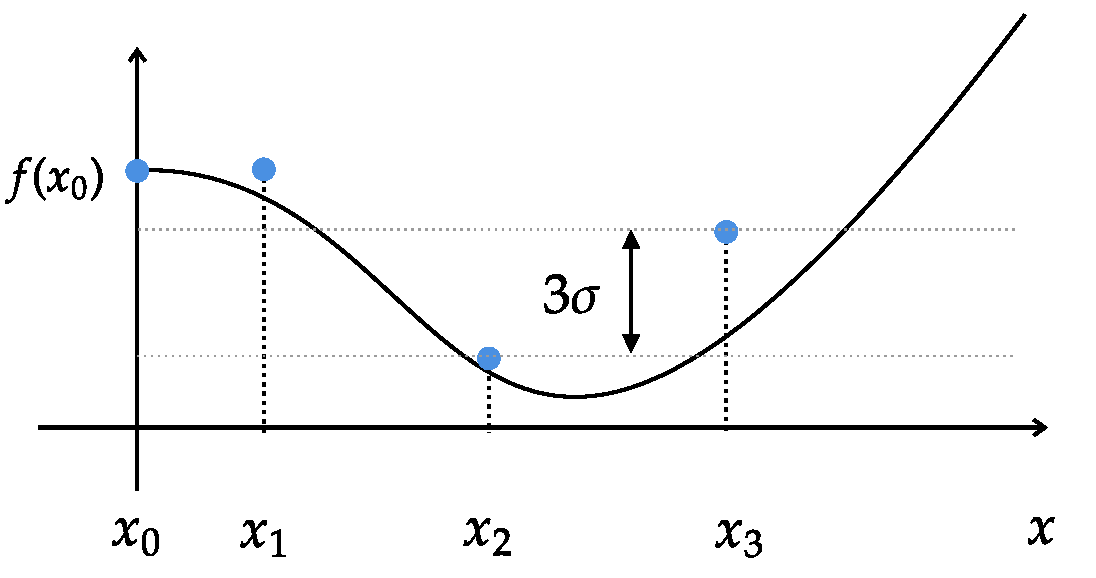
\includegraphics[width=\textwidth]{Images/bracketing.pdf}
        \caption[Illustration of RCDS bracketing.]{Illustration of RCDS bracketing. Black curve is the objective function, blue dots are its measurements, with noise. Bracketing routine: scan the objective function downhill, updating the guess for the minimum, until $f$ stops decreasing and increases by more than $3\sigma$ compared the minimum.}
        \label{fig:bracketing}
    \end{minipage}
    \hfill
    \begin{minipage}{0.48\textwidth}
        \centering
        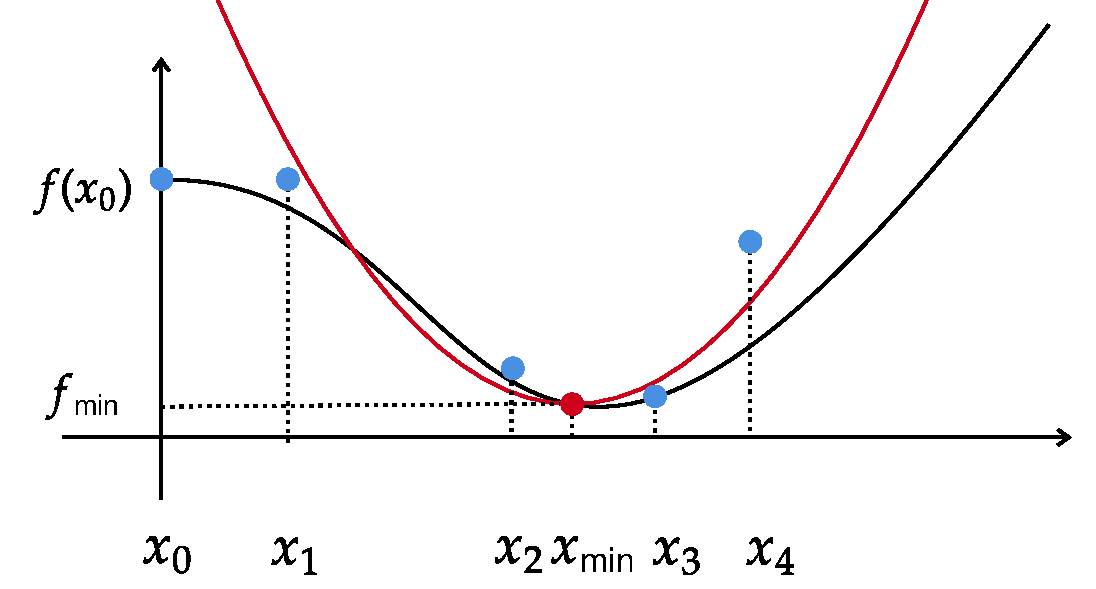
\includegraphics[width=\textwidth]{Images/linescan.pdf}
        \caption[Illustration of RCDS line-scan procedure.]{Illustration of RCDS line scan procedure: perform a parabolic fitting (red curve) over a curated set of objective function measurements (blue dots) within the brackets. Outliers are removed, if any is present. The parabola vertex is the best guess for $f$'s minimum.}
    \end{minipage}
\end{figure}
\subsection{Powell's conjugate directions}
How could we optimize an objective function $f(\vb{x})\in\mathbb{R}$ depending on the set of $p$ parameters $\{x_i\}_{i=1,\dots,p}$? The simplest idea is to iteratively nudge each knob individually: optimize $f$ by changing $x_1$, while the other knobs remain fixed, then optimize by changing $x_2$ only, and so forth. In other words, since each one of the knobs defines a direction whose basis vector is $\vu{e}_i$, we could scan each direction, one at once, using the noise-robust line-optimizer introduced in the previous section.

Formally, we are reducing a multi-dimensional optimization problem into a series of 1-dimensional searches. That is, given an initial configuration of the parameters (an initial position) $\vb{x}_0$, and a direction $\vu{n}$, we have the one-dimensional problem to minimize $g(\delta)=f(\vb{x}_0 + \delta \vu{n})$. The minimum is  then $f(\vb{x}_0 + \delta_* \vu{n})$, where $\delta_* = \text{argmin}_\delta g(\delta)$. In the scheme of the previous paragraph, we specialized to $\vb{n}=\vu{e}_i$, and iterated for $i=1,\dots, p$.

\begin{figure}[htb]
    \centering
    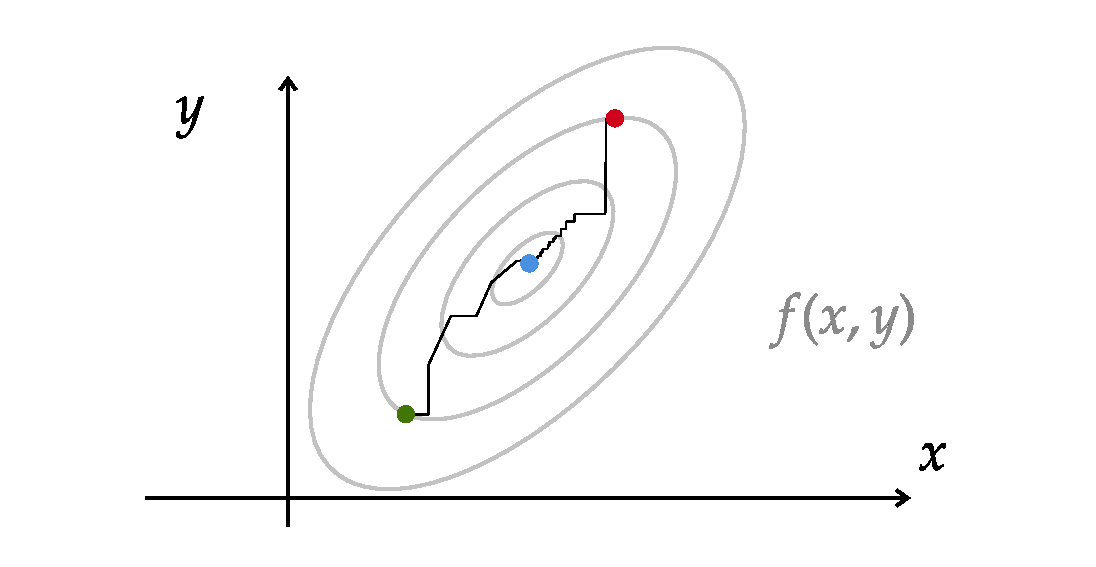
\includegraphics[width=0.9\textwidth]{Images/powell_loop.pdf}
    \caption[Comparison of iterated line-searches until $f(x,y)$'s minimum along canonical unit vectors vs. along vectors chosen according to Powell's method.]{Comparison of iterated line-searches until $f(x,y)$'s minimum along canonical unit vectors (path from red dot to blue dot) vs. along vectors chosen according to Powell's method of conjugate directions (path from green to blue dot).}
    \label{fig:powell}
\end{figure}

As can be seen in the path from the red point to the blue point in fig.~\ref{fig:powell}, scanning along each orthogonal canonical direction can be time-consuming, specially for some functions with long and narrow valleys at some angle with the coordinates basis vectors.
% This strategy thus is sub-optimal when evaluation of the objective function is expensive, which is our case, since, as the next chapters discuss, our objective function always involves firing an injection pulse into the storage ring.
The reason why using unit basis vectors can be so inefficient is because optimizing along a given basis vector spoils down the prior minimization carried out in other directions. As a result, the process requires more iterations to crawl to the minimum.

Instead of canonical directions, a more efficient strategy for optimizing consists on constructing a set of special, non-interfering direction vectors for which the minimization along a direction is preserved when optimizing in a different direction.
% Going back to the one-dimensional problem of minimizing along a direction $\vb{u}$, $\delta_* = \text{arg min}\ g(\delta) = f(\vb{x}_{0}+\delta\vu{u})$, we know that, at the minimum, we must have vanishing derivative: $g^{\prime}(\delta_*)=\grad f(\vb{x}_{0}+ \delta_* \vu{u})\cdot \vu{u}=0$. Therefore, the gradient is perpendicular to $\vu{u}$ at $\delta_*$.
% Consider now the quadratic-form approximation for the objective function around point $\vb{x}_0$, taken as the origin.
% \begin{equation}
%     f(\vb{x})=f(\vb{x}_0)+\grad f(\vb{x}_0)\cdot \vb{x} + \frac{1}{2}\vb{x}\cdot\vb{H}(\vb{x}_0)\cdot\vb{x},
% \end{equation}
% where, as usual, $(\grad f(\vb{x}_0))_i = \pdv*{f(\vb{x}_0)}{x_i}$ is the gradient, and $(\vb{H})_{ij} = \pdv*{f(\vb{x}_0)}{x_i}{x_j}$ is the Hessian matrix. Up to such approximation, differentiation of the previous expression reaveals the gradient can be approximated by
% \begin{equation}
%     \grad f(\vb{x}) = \grad f(\vb{x}_0) + \vb{H}(\vb{x}_0)\cdot \vb{x}
% \end{equation}
% and thus is changed by
% $$\delta(\grad f ) = \vb{H}(\vb{x}_0)\cdot \delta \vb{x}$$
% upon a step $\vb{\delta \vb{x}}$. Suppose we have optimzed along direction $\vb{u}$, so $\grad f(\vb{u}) = \grad f(\vb{x}_0) + \vb{H}\cdot \vb{u}$. Now, optimizing along $\vb{v}$ will be non-interfering if the gradient stays orthogonal to $\vb{v}$, that its
In ref.~\cite{press_numerical_2007} the properties that these desired non-interfering vectors should have is discussed. It is shown that the necessary condition for direction vectors $\vb{u}$ and $\vb{v}$ to be non-interfering is
\begin{equation}
    \vb{v}\cdot\vb{H}\cdot\vb{u}=0,
\end{equation}
where $(\vb{H})_{ij} = \pdv*{f(\vb{x}_0)}{x_i}{x_j}$ is the Hessian matrix for the objective function $f$. The $\vb{u}$ and $\vb{v}$ directions are said to be \textit{conjugate} directions.

The question now is on how to find this appropriate set of $p$ conjugate directions. Let $\{\vb{u}_i\}$ denote our directions set. Powell \cite{powell_efficient_1964} proved that conjugate directions can be obtained according to the following algorithm:
\begin{enumerate}
    \item Let the initial directions be the basis vectors: $\vu{u}_i=\vu{e}_i$ for $i=1,\dots, p$.
    \item Save the starting point (initial parameters state) as $\vb{x}_0$;
    \item For $i=1,\dots, p$ minimize along $\vu{u}_i$. Save the minimum as $\vb{x}_i$.
    \item For $i=1,\dots p-1$ set $\vu{u}_i\leftarrow\vu{u}_{i+1}$
    \item Set $\vb{u}_p=\vb{x}_p - \vb{x}_0$. Normalize to obtain $\vu{u}_p$.
    \item Minimize along $\vu{u}_p$. Name the found minimum as the new $\vb{x}_0$.
    \item Repeat the procedure until reaching a certain number of evaluations or until some stopping condition is reached.
\end{enumerate}

In steps 1--3, we optimize along each one of the unit basis vectors, updating the minimum. When finishing optimization along $\vb{u}_p$, the current minimum will be $\vb{x}_p$. In step 4 we discard the first direction, rename directions $\vb{u}_{i+1}$ to $\vb{u}_i$, and set as our new $p$-th direction the vector pointing along the line from the starting point $\vb{x}_0$ to the the current minimum.

In this loop, steps 1--6 characterize 1 iteration and results in 1 new direction. Powell proved that, for a quadratic form, $k$ iterations of this strategy produces a set of directions whose last $k$ vectors are mutually, pairwise conjugate, in the sense of the Hessian matrix. So $p$ iterations exactly minimizes the quadratic form. The method is also quadratically convergent: each iteration doubles the number of significant figures of the candidate minimum for the quadratic form.

There is a problem, however, in throwing away  for $\vu{u}_1$ for $\vb{x}_p - \vb{x}_0$ every iteration: at some point the lines start to fold up on each other and lose linear independence. As a result the function can end up minimized only within a subspace of parameter space. To fix this, you can reinitialize the directions to the basis vectors after an iteration along the $p$ directions, or use any new set of orthogonal directions. This means giving up conjugacy and quadratic convergence.

The apparently counter-intuitive solution suggested by Powell is to discard not necessarily $\vu{u}_1$ in favor of the new direction, but the direction along which $f$ had its largest decrease so far. This is justified because this direction is likely have a large component along the new proposed  direction. Powell also posits some conditions in which is best not to add any new directions, keeping the old set from the previous iteration \cite[section 10.7]{press_numerical_2007}. The resulting algorithm shall is referred to as "Powell's method".

Powell's method results in a set of $p$ directions which are no longer mutually conjugate by the end of $p$ iterations. The search is also no longer quadratically convergent, but it is more adequate for more diverse objective function landscapes. For instance, if the objective function has long, twisting valleys, quadratic convergence guaranteed by conjugate directions is of no use since we  may start far away from the nearly parabolic region. In this situation, we would be leaping along the minimum of a parabola which is not quite at the minimum yet. When close to "true" parabolic region, Powell's criteria results in adequate directions which tends to crawl about the paraboloid principal axes quite efficiently.

The path from the green to the blue point in fig.~\ref{fig:powell} illustrates the use of Powell's method for choosing directions. In it, we can see that the two initial search directions were performed along the unit canonical vectors. Next, the direction pointing from the starting point to the minimum after the two first searches is used, and the direction with the largest component along it, $\vb{e}_y$, was discarded. Further iterations rendered directions along which the search tends to walk by the principal axis of the paraboloid in a more efficient manner than the searches using unit canonical vectors.

In summary, Powell's method calculates and manages directions adaptively, deciding when to change old directions in favor of the newly calculated  vectors, and when to avoid the changes to control build-up of linear dependence. In practice, using Powell's directions accounts to finding a good set of directions providing "shortcuts" towards the minimum in the objective landscape, instead of "zig-zags", as for the case of canonical vectors.

RCDS consists on using Powell's method for managing directions and minimizing along these directions with the noise-robust line-optimizer described previously. RCDS was first implemented by the authors of ref.\cite{huang_algorithm_2013} and is available in Matlab and Python in their \href{https://github.com/SPEAR3-ML/RCDS}{GitHub repository}. The code used on SIRIUS was based on their implementation. The SIRIUS code is object-oriented and was  implemented in Python by members of the Accelerator Physics Group of the Brazilian Synchrotron Light Laboratory (LNLS) and the author. The code is available in the "optimization" directory of the \href{https://github.com/lnls-fac/apsuite}{Accelerator Physics Suite (apsuite)} repository \cite{apsuite}. The pseudocode for the bracketing and line scan routines as well as Powell's directions loop is available in \ref{chap:pseudocode}.

\chapter{Storage ring setup, diagnostics, measurements \& experimental methods}
In this chapter, we delve into the SIRIUS magnetic lattice, beam diagnostics tools and relevant experimental methods. We emphasize the key parameters  for optimizing nonlinear dynamics and detail the experimental procedures encompassing beam trajectories and orbits, beam current and lifetime, as well as the control and manipulation of tunes and chromaticity during machine studies. The final segments address the selection of objective functions for probing the Dynamic Aperture and the selection of sextupole families as optimization knobs.

\section{SIRIUS magnetic lattice}
\label{sec:mag_latt}
SIRIUS storage ring consists on a 20-cell \gls*{5ba} lattice comprising a 5-fold symmetric configuration with alternating high and low horizontal betatron functions at the straight sections, as Fig.~\ref{fig:5BA_lattice} shows. There are 5 A-type sections, with high horizontal betatron function and 15 B- and P-type sections, with low horizontal and vertical betatron functions \cite{liu_new_2016}.
% While the B and P sections share identical linear lattice elements (dipoles and quadrupoles\footnote{The quadrupole families are in fact distinct. Their strengths can be changed and this symmetry can be broken. Currently the strengths of the quadrupoles in the B and P sections are the same.}), they differ in their sextupoles.
A superperiod consists of one high-beta and 3 low-beta sections arranged in the order A-B-P-B.
% Among the 20 straight sections, 17 are allocated for insertion devices (IDs), 2 for machine installations, and 1 for shared use between a small ID and machine installation [21].

The central dipole, the BC, is a permanent superbend magnet with a peak field of $3.2~\unit{T}$. The storage ring accommodates 20 such. The arcs contain additional four dipoles: two B1 and two B2. These are electromagnetic dipoles with peak fields of $0.58~\unit{T}$. In total, the SIRIUS magnetic lattice comprises 100 dipoles: 20 permanent BC magnets and 80 B1 and B2s electromagnets.

In the high-beta straight sections, the quadrupole doublet (QFA, QDA) is employed for optics matching. B-type sections utilize the (QDB1, QFB, QDB2) quadrupole triplet for matching while the (QDP1, QFP, QDP2) triplet is used in the P-type sections. The arc sections contain the Q1, Q2, Q3, and Q4 quadrupole families, totalling 12 families of quadrupoles and 270 magnets.

The lattice also features 21 families of sextupoles magnets, used for chromaticity correction and nonlinear dynamics optimization. They sum up to 280 magnets. Some sextupoles families are located where the dispersion function vanishes and are called \textit{achromatic}, or harmonic, while other families, located where there is non-zero dispersion, are called \textit{chromatic} families.

Table~\ref{tab:sext_fams} lists the sextupoles families and their types in the storage ring. The 21 families are, in principle, the available search space for nonlinear dynamics optimization. The subsection~\ref{subsec:knobs}, on the choice of optimization knobs, at the end of this chapter, shows how the search space can be reduced down to 13 dimensions once the constant chromaticity requirement and/or other additional constraints are imposed.

\begin{figure}[htb]
    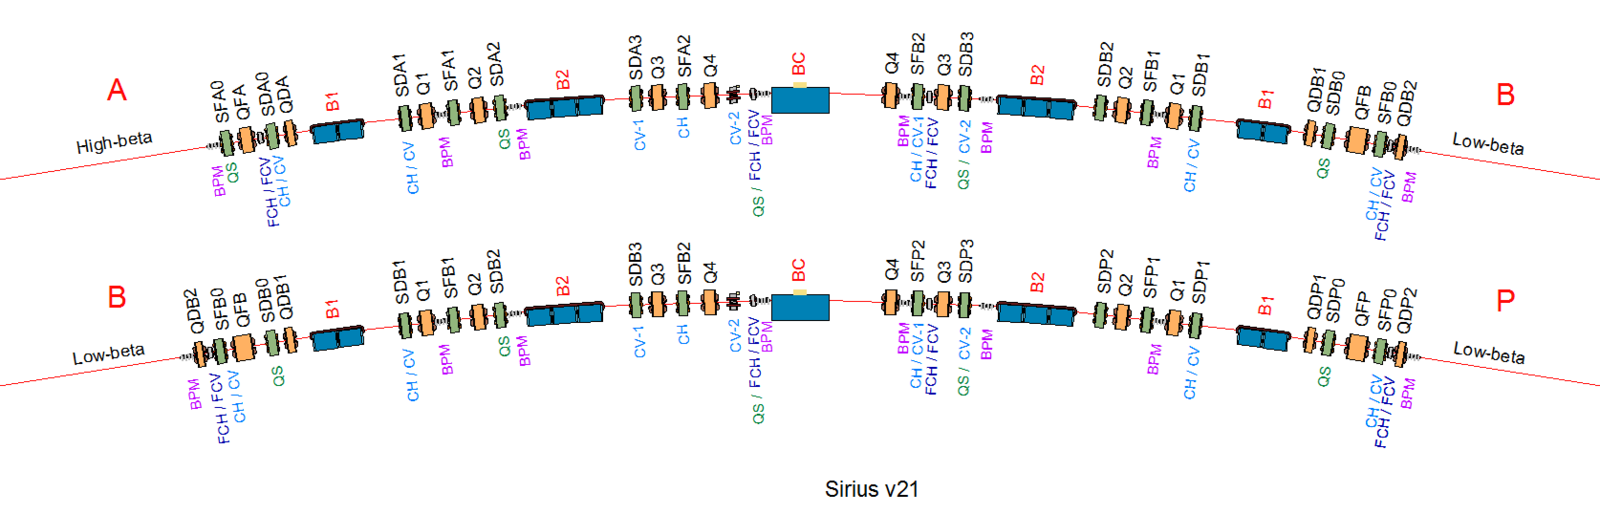
\includegraphics[width=\textwidth]{Images/sirius_arcs.png}
    \caption[SIRIUS 5BA cells comprising the lattice.]{SIRIUS \gls*{5ba} cells comprising the lattice. The cells differ by their straight section types: high-beta type (A), or low-beta (B, P). A superperiod consists of one high-beta and 3 low-beta sections arranged in the order A-B-P-B. The storage ring consists on 5 concatenation of superperiods. Source: Wiki-SIRIUS (currently only available on-campus).}
    \label{fig:5BA_lattice}
\end{figure}

\begin{table}[htb]
    \caption{SIRIUS sextupole families}
    \centering
        \begin{tabular}{ll}
        \hline
        achromatic                                                                      & chromatic                                                                                                                                          \\ \hline
        \begin{tabular}[c]{@{}l@{}}SFA0, SDA0, SFB0,\\ SDB0, SDP0, SFP0\end{tabular} & \begin{tabular}[c]{@{}l@{}}SDA1, SFA1, SDA2, SFA2,SDA3, SDB1, SFB1,\\ SDB2, SFB2, SDB3, SFP1, SDP1, SDP2, SFP2, SDP3\end{tabular}
        \end{tabular}
        \label{tab:sext_fams}
\end{table}

% For coupling control and the beam-based alignment (BBA) process \cite{cruz_aplicacoes_2022} there are 5 skew quadrupoles (QS) per arc, totaling 100 QS in the storage ring. At each arc, 4 of the QS are realized as additional coils in sextupole magnets and account for coupling, while the other, immediately before the BC, is realized in a dedicated corrector magnet and required for BBA.

% Besides the lattice magnets, SIRIUS has correction dipole magnets distributed among the two types of correction systems available: fast orbit correction and slow orbit correction. Both of them share the same orbit diagnostic device probing the beam's centroid positions: beam position monitors (BPMs). Each arc section is equipped with 8 BPMs, totaling 160 BPMs in the storage ring.  For the slow orbit correction system, each section has 6 horizontal correctors (CH) and 7 vertical correctors (CV), both installed in sextupole magnets. An extra vertical corrector magnet is installed per arc, resulting in 120 CHs and 160 CVs in the storage ring.

% The fast orbit correction system comprises 4 horizontal and 4 vertical fast correctors (FCH and FCV, respectively) per sector, totaling 80 FCH and 80 FCV (2 FCH and 2 FCV per source point). The Slow Orbit Feedback system (SOFB) and the Fast Orbit Feedback (FOFB) system currently oversee the slow and fast orbit corrections simultaneously.

\section{Beam diagnostics and measurements}
\subsection{Beam positions}
To track the beam's position along the ring, a diagnostic tool known as \gls*{bpm} employs a set of four pick-up antennas positioned within the vacuum chamber, as illustrated by Fig~\ref{fig:bpms_scheme}. The mirror charges induced by the electron beam are collected by the antennas. The determination of beam displacements relies on the differential signal induced on the antennas when the beam deviates from the device's geometric and electric center. The induced voltage signal undergoes processing in the "partial-Delta/Sigma" scheme, providing horizontal and vertical beam displacements through the following algebraic calculations:
\begin{equation}
    x = K_x \qty[\frac{A-C}{A+C}+\frac{D - B}{D+B}], \quad y = K_y \qty[\frac{A-C}{A+C}-\frac{D - B}{D+B}],
\end{equation}
where $A$, $B$, $C$, and $D$ represent the intensity of the induced signal over the corresponding antennas and $K_x$ and $K_y$ calibration factors. 

SIRIUS is equipped with 160 \gls*{bpm} distributed along the storage ring. The \glspl*{bpm} allow the determination of the centroid's (beam electric center) displacements at a turn-by-turn (\gls*{tbt}) acquisition rate for probing the betatron motion. The signal can also be processed at other acquisition rates, allowing for signal averaging and providing information about the orbit.
\begin{figure}
    \centering
    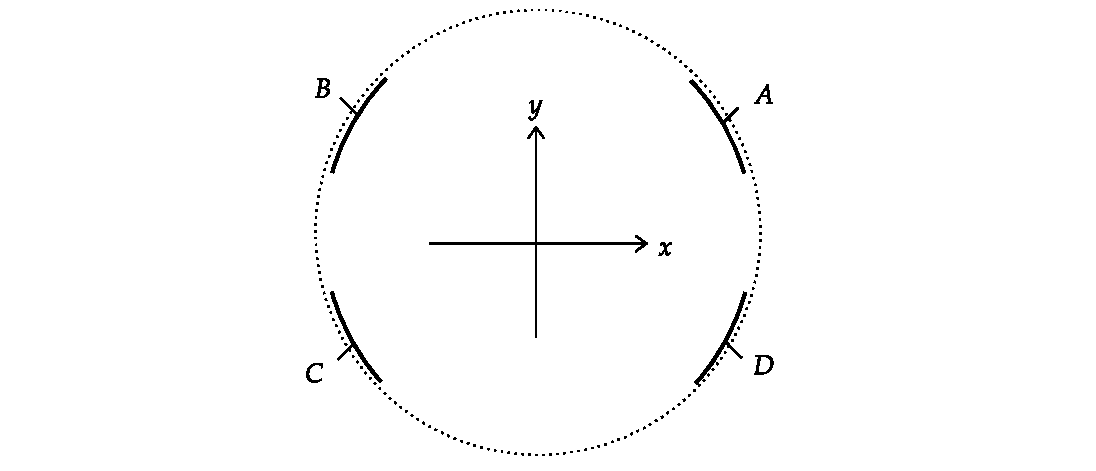
\includegraphics[width=\textwidth]{Images/bpm_scheme.pdf}
    \caption[Schematic representation of BPM button antennas, the vacuum chamber cross-section, and the transverse positions reference frame.]{Schematic representation of \gls*{bpm} button antennas, in solid lines, the vacuum chamber cross-section, in dashed lines, and the transverse positions reference frame.}
    \label{fig:bpms_scheme}
\end{figure}
\subsubsection{Phase-space reconstruction and decoherence}
With \gls*{bpm} recording the \gls*{tbt} motion of the beam's centroid, the $x$ and $y$ positions can be readily acquired. The angles, or momenta, can be obtained through the following processing: for two consecutive \glspl*{bpm} located at the ends of a straight section of length $\ell$, where no bending or focusing occurs, the beam angle can be calculated as $x^\prime = \frac{\Delta x}{\ell}$, where $\Delta x$ refers to the difference in the \glspl*{bpm} position readings. This allows for the reconstruction of the $x, x^\prime$ and $y, y^\prime$ phase-spaces on a \gls*{tbt} basis, as exemplified by Fig.~\ref{fig:phase_space_recons}. In the figure, \gls*{bpm} data of the beam was acquired at the \gls*{tbt} rate, soon after betatron oscillations were induced to the beam's centroid. The beam initially had an amplitude in the negative horizontal direction reaching approximately $-8~\unit{mm}$ and in the first turns it circulated the outermost region of the phase portrait (dark blue points). The last turns correspond to light yellow points in the innermost region.
\begin{figure}
    \centering
    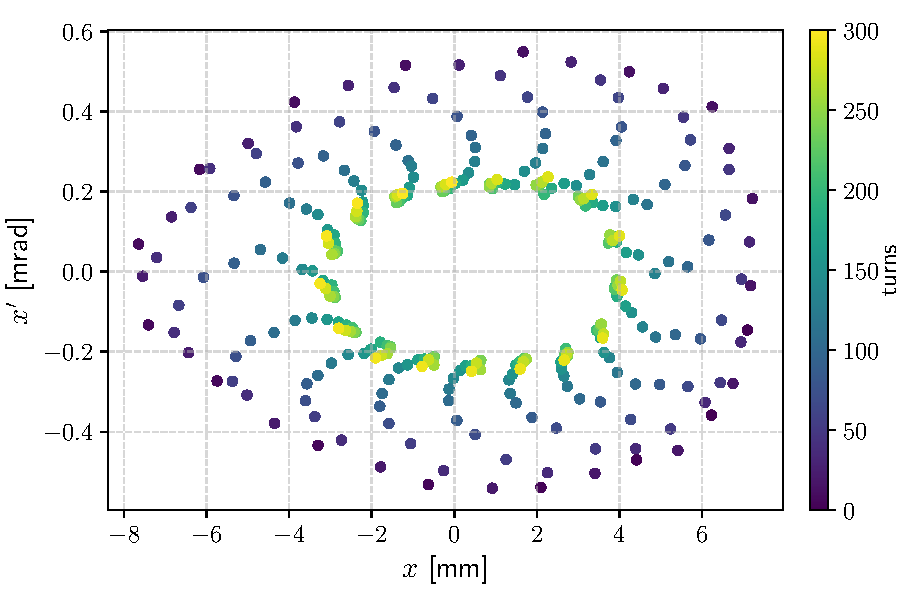
\includegraphics[width=0.7\textwidth]{Images/phase_space_recons.pdf}
    \caption[Phase space reconstruction from TbT BPM data.]{Phase space reconstruction from \gls*{tbt} \gls*{bpm} data. Data was collected for 300 turns in the storage ring. The color-scheme encodes the turn each point was collected.}
    \label{fig:phase_space_recons}
\end{figure}

At first glance, in Fig.~\ref{fig:phase_space_recons}, it might seem that the transverse positions are being damped. However, the radiative damping time for the SIRIUS storage ring is of the order of thousands of turns, much more than the acquired time scale in the figure. This apparent damping is a manifestation of \textit{decoherence}. Decoherence arises due to the nonlinear tune-shifts and the finite extent of the beam in 6-dimensional phase space, which has a spread over amplitudes. The cumulative effect of amplitude-dependent and momentum-dependent tune-shifts renders the bunch with a spread in tunes. This results in the filamentation and spreading of an initially localized bunch in phase space due to the different frequencies (the tunes) with which they circulate the ellipses. In this scenario, the positions (and momenta) tend to become uncorrelated, and the average of the electrons distribution, which is the beam's centroid measured by the \glspl*{bpm}, goes to zero, justifying the apparent damping.
\subsection{Beam current and injection efficiency}
\glspl*{dcct} enable the measurement of the stored beam current within accelerator rings (booster or storage ring). The \glspl*{bpm} sum-signal, which is proportional to the beam current, can also be used to measure currents and calculate current variations. In transport lines, there are also Integrated Current Transformers (ICTs) which allow measuring the integrated current (charge) per pulse.
% A \glspl*{dcct} current monitor works by surrounding the beam of charged particles in the accelerator ring with a magnetic core. The magnetic field induced by the beam current flowing through the core is then measured, allowing for an accurate determination of the passing current.

Utilizing the current measurement and the beam revolution period in the respective ring, one can assess the stored charge and calculate the injection efficiency (\gls*{ie}) during storage ring injections. By measuring the charge in the booster or transport line just before injection into the storage ring and the storage ring charge immediately after the injection pulse, it is possible to deduce the efficiency of the injection process.
\subsection{Tunes measurement \& control}
When \gls*{tbt} motion is viewed at a fixed longitudinal position $s$, it consists of the sampling of a harmonic motion, for which the fundamental frequency is the fractional part of the tune $\nu$. Thus, observation of \gls*{tbt} data can reveal the tunes upon the appropriate signal processing. For instance, the betatron motion can be Fourier-transformed (discrete Fourier transform via fast-Fourier transform algorithm), revealing the \gls*{bpm} signal spectrum. Alternatively the time-domain signal can be fitted to a sinusoid, allowing the determination of the tune as the fundamental frequency.

Despite being simple, the process described above is incompatible with user's shift operation, and mostly used during machine experiments for measuring the tunes of large-amplitude motion or for precise determination of changes in tune due to relevant changes in operation parameters. The main incompatibility with user's operation is that extracting tunes from \gls*{tbt} data requires inducing betatron oscillations by kicking and the beam and operating with the \glspl*{bpm} in the \gls*{tbt} acquisition rate. This means the control loops of the \gls*{fofb} and \gls*{sofb}, which guarantee the orbit stability required by the beamlines, must be turned-off. 

Precise  monitoring of the tunes during operation is achieved with the aid of a strip-line shaker, which constantly drives the beam with an alternating electric field in a narrow band of frequencies, leading to sub-nanometer displacements and inducing small-amplitude betatron motion without interfering significantly with the operation. This system also reads back the beam response at that same frequency range. The peak of the beam response signal is identified with the betatron tune.

Regarding changes and manipulation of the tunes, formula~\eqref{eq:delta_nu} reveals that adjustments in the quadrupole strengths, particularly at the quadrupoles in large $\beta$-function sections, enable control of the tunes. As the tune response to changes in quadrupole strength is linear, a tune-response matrix can be constructed, i.e., the Jacobian of the tunes with respect to changes in quadrupoles, allowing tune changes to be expressed as
\begin{equation}
    \Delta\boldsymbol{\nu} = \vb{J}_{\boldsymbol{\nu}}\Delta \vb{K},
    \label{eq:delta_nu_jac}
\end{equation}
where $\Delta\boldsymbol{\nu} = \mqty*[\Delta \nu_x & \Delta \nu_y]^\intercal$ is the tune-shifts vector, $\Delta \vb{K}$ is the vector containing the changes in strengths across all the quadrupole families, and the Jacobian or response matrix has entries
\begin{equation}
    (\vb{J}_{\boldsymbol{\nu}})_{ij} = \pdv{\nu_{i}}{K_j} \approx \frac{\Delta \nu_{i}}{\Delta K_j}, \quad i=x, y,\quad j\in\text{tune-correction quadrupole families}.
\end{equation}
The system~\eqref{eq:delta_nu_jac} can pseudo-inverted, allowing for the determination of quadrupoles changes required for a desired change in tune
\begin{equation}
    \Delta \vb{K} = \vb{J}_{\nu}^{+}\Delta \boldsymbol{\nu}
\end{equation}
where $\vb{J}_{\nu}^{+} = (\vb{J}_{\nu}^{\intercal}\vb{J}_{\nu})^{-1}\vb{J}_{\nu}^{\intercal}$ is the Moore-Penrose pseudoinverse. 
The tune-correction quadrupole families are located in non-dispersive sections 
% \todo[inline]{add discussion on how the optics changes when changing tunes}
\subsection{Chromaticity measurements \& control}
Chromaticity characterizes the energy-dependent tune-shift. To measure it, we need to calculate the numerical derivative
\begin{equation}
    \xi_u = \pdv{\nu_u}{\delta}\approx \frac{\Delta \nu_u}{\delta}, \quad u=x, y,
    \label{eq:chrom_numerical}
\end{equation}
that is, measure the tune-shift $\Delta \nu_u$ induced by the energy-shift $\delta$.

A direct manner to induce a particular energy-shift is to change the RF cavities frequency. A relation can be established between energy deviations $\delta$ and relative RF frequency changes with the aid of a quantity $\alpha$, known as \textit{momentum compaction factor} \cite{lee_accelerator_2004,sands_physics_1969}:
\begin{equation}
    \delta = -\frac{1}{\alpha}\frac{\Delta f}{f}.
    \label{eq:delta_frequency}
\end{equation}
Where the momentum compaction factor is defined by
\begin{equation}
    \alpha \equiv \frac{1}{L}\oint G(s) \eta(s) \dd{s},
\end{equation}
and is first introduced to relate changes in orbit length due to energy deviations \cite{sands_physics_1969}.

Therefore, in practice, when measuring chromaticity, we are interested in the following numerical derivative, which is a consequence of eqs.~\eqref{eq:chrom_numerical} and \eqref{eq:delta_frequency}:
\begin{equation}
\xi_u = -\frac{f}{\alpha}\frac{\Delta \nu_u}{\Delta f}.
\end{equation}
The derivative is usually calculated by obtaining the first-degree coefficient of the polynomial fitting of the tune-shifts vs. RF frequency curve.

Regarding chromaticity control, eq.~\eqref{eq:chromaticity} shows that chromaticity depends linearly on the strengths of the chromatic sextupole families. Thus it can be adjusted to certain desired values according to the same pseudo-inversion procedure described above for the tunes. We relate the changes in chromaticity $\Delta \boldsymbol{\xi}$ to the changes in the strengths of the sextupole families $\Delta \vb{S}$ by
\begin{equation}
    \Delta\boldsymbol{\xi} = \vb{J}_{\boldsymbol{\xi}}\Delta \vb{S},
\end{equation}
where $\Delta\boldsymbol{\xi} = \mqty*[\Delta \xi_x & \Delta \xi_y]^\intercal$ and the Jacobian matrix $\vb{J}\in$ has entries
\begin{equation}
    (\vb{J}_{\boldsymbol{\xi}})_{ij} = \pdv{\xi_{i}}{S_j} \approx \frac{\Delta \xi_{i}}{\Delta S_j},\quad i=x, y, \quad j\in\text{chromaticity correction sextupole families}.
\end{equation}
% $d_s$ refers to cardinality of the set of sextupole families used in the chromaticity change process.In principle, at least two families are required for correcting/tuning chromaticity in the machine: one family for each plane. Since the chromatic sextupole families are the only ones effectively changing chromaticity to leading order, then, at most, $d_s=15$.

If we wish to change chromaticity by a $\Delta\boldsymbol{\xi}$ amount, the Jacobian can be pseudo-inverted to calculate the required sextupole strength changes:
\begin{equation}
    \Delta \vb{S} = \vb{J}_{\xi}^{+}\Delta \boldsymbol{\xi}.
\end{equation}
In practice, the chromaticity Jacobian was never measured in the actual machine, due to the time-consuming process of varying each sextupole family individually and carrying out the chromaticity measurement. The "measurement" of the Jacobian is instead carried out in the SIRIUS storage ring computer model. The model-calculated Jacobian renders satisfactory chromaticity corrections in the actual machine.

\section{The choice of objective function \& optimization knobs}

\subsection{The objective function}
\label{subsec:objective_function}
There is no analytical formula relating the storage ring linear or nonlinear optics to the Dynamic Aperture (\gls*{DA}). The optimization procedure must be a heuristic search procedure: changes are performed to the knobs (nonlinear magnets) and the effect on the \gls*{DA} is evaluated. Additionally, one cannot measure the \gls*{DA} in a practical and straightforward measurement procedure sufficiently fast to be run online. Direct measurements of \gls*{DA} can take several iterations of acquiring trajectories of the beam with increasingly higher transverse displacements. The acquisitions are then processed to access the \gls*{DA}.

\begin{figure}
    \centering
    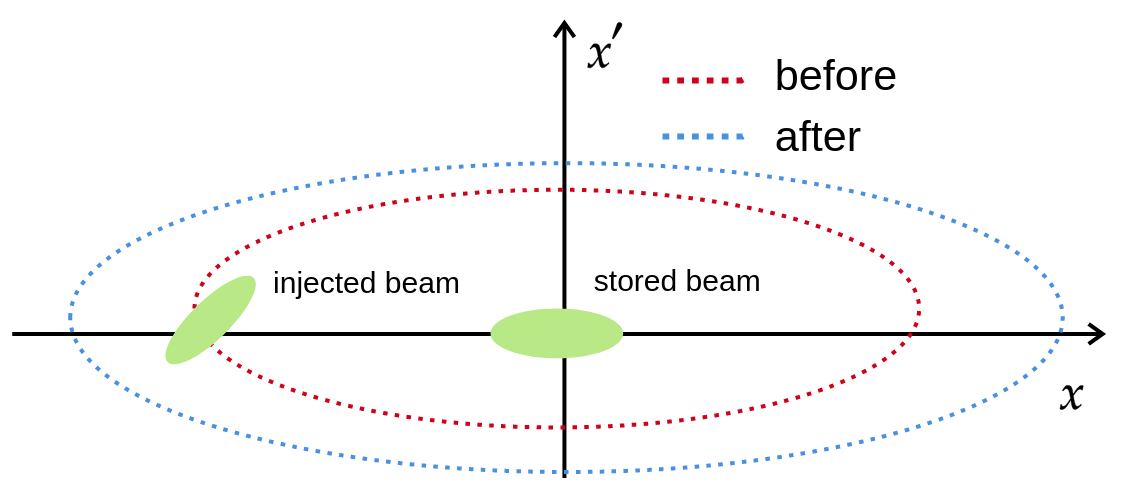
\includegraphics[width=0.7\textwidth]{Images/injection_illustration.png}
    \caption[Illustration of injection sensitivity to the DA]{Illustration of injection sensitivity to the \gls*{DA}. In red, the \gls*{DA} border before optimizing sextupoles. In blue, the expected effect on the \gls*{DA} border after optimization. Reduced injection efficiency results from losing part of the beam due to small \gls*{DA}. Optimizing injection efficiency by tuning sextupoles should translate to optimizing \gls*{DA}.}
    \label{fig:injection_efficiency}
\end{figure}

For online optimization one must choose a practical, relatively fast to measure objective function to act as a probe of the \gls*{DA}: a figure of merit related to the \gls*{DA} to represent it and to be used to evaluate the quality of the changes performed during the online tuning process. In our experiments, we studied using two practical objectives as the probes for \gls*{DA}: the \textbf{injection efficiency} (\gls*{ie}) and the \textbf{beam's resilience to dipolar perturbations}. The former is quite self-explanatory: the larger the \gls*{DA}, larger the space for the beam to be captured into the storage ring during the injection pulse, and thus the larger the injection efficiency.

Figure~\ref{fig:injection_efficiency}  illustrates how a smaller aperture, shown in red, influences the efficiency of injection. After leaving the booster accelerator at $3~\unit{GeV}$, the beam is transported into the storage ring injection straight section. It reaches the injection area with phase space coordinates of approximately $(x, x^\prime)\approx(-8~\unit{mm}, 3~\unit{m rad})$. The beam then suffers the deflection of a nonlinear pulsed magnet, the \gls*{nlk} and is captured into the storage ring with phase space coordinates $(-8~ \unit{mm}, 0)$ \cite{liu_injection_2016}. If the \gls*{DA} border along the negative horizontal direction is reduced below $-8~\unit{mm}$, the dynamics may not accommodate the long term time evolution of the beam fraction exceeding this threshold. This fraction is lost due to the nonlinear dynamics instabilities in the first turns. On the other hand, if the \gls*{DA} is increased, the larger the beam fraction which is successfully captured and survives in the storage ring in the long term.

As for the beam kick resilience, this figure of merit is related to the \gls*{DA} by the following reasoning: the larger the horizontal dipolar kicks the beam can survive, the larger the orbit distortions towards the positive or negative horizontal direction (depending on the kick direction). So the larger the amplitudes the beam explores as it oscillates. If the beam survives to larger kicks, it means the ring can accommodate larger orbit distortions because of an increased \gls*{DA}.

Figure~\ref{fig:action_jump} illustrates the phase space orbits for a beam when it is kicked. In the left sketch, small amplitude \gls*{tbt} motion ellipse is shown. When kicked, the beam gains momentum (angle) and is rigidly translated higher along the $x^{\prime}$ direction. In the linear approximation the beam goes from one ellipse, with action $J$ to another ellipse, with action $\tilde{J}>J$. If the kick is stronger (larger than $500~\unit{\mu rad}$), the action jump takes the beam to a nonlinear regime, as shown in the right sketch, where the beam traces out distorted ellipses. After the kick, the maximum amplitude reached in the negative horizontal direction is increased thus the larger the fraction of the beam that can survive the kick, the larger the \gls*{DA}.

\begin{figure}
    \centering
    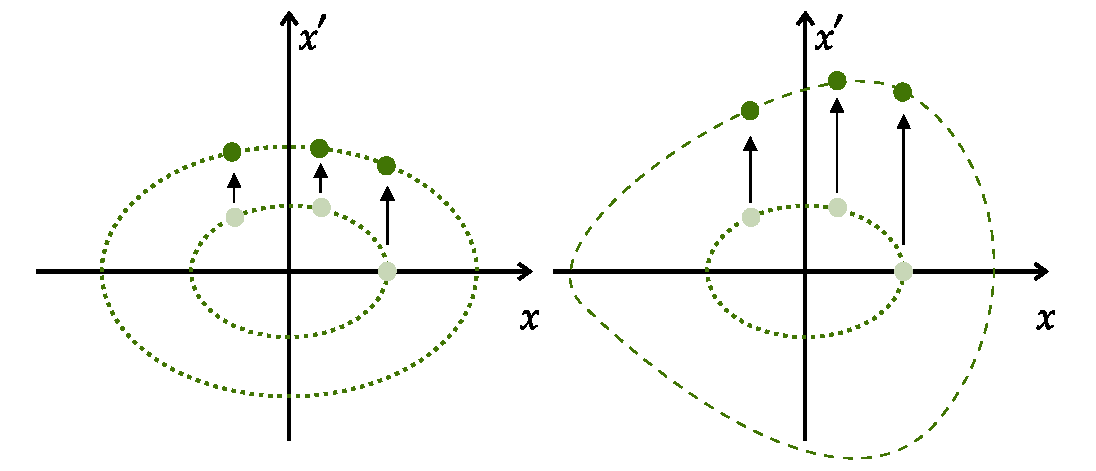
\includegraphics[width=\textwidth]{Images/phase_space_kick.pdf}
    \caption[Action jumps due to dipolar kicks in the linear and nonlinear regimes.]{Action jumps due to dipolar kicks in the linear (left) and nonlinear (right) regimes.}
    \label{fig:action_jump}
\end{figure}

% \subsection{Injection scheme for acummulation at SIRIUS storage ring}
% Beam acummulation into the storage ring occurs in the off-axis scheme. The beam is delivered at $x\approx-8~\unit{mm}$, and receives the kick from the nonlinear kicker field. The field profile is nonlinear, with zero field and gradient at the center of the axis, so that it does not disturbs the stored beam.
% In the off-axis scheme, a sufficiently large dynamic aperture is desired to allow the beam to be captured into the storage ring. The predicted efficiency for SIRIUS setup, considering a dynamic aperture reaching $x=-9~\unit{mm}$, was nearly $100\%$. What was observed during 2022 was an injection efficiency of about $88\pm8\%$.

In summary, the dynamic aperture optimization procedure must consist on the exploration of sextupole (knobs) configurations yielding the largest dynamic aperture as accessed by as objective function such as injection efficiency or beam kick-resiliency.

\subsection{The optimization knobs}
\label{subsec:knobs}
The \gls*{DA} is determined by the quality of the beam dynamics in terms of perturbations. Given that a linear optics correction scheme is already in place and regularly implemented in the machine, effectively addressing optics functions and phase advances, the primary factor impacting SIRIUS \gls*{DA} likely stems from nonlinear dynamics and/or remaining uncorrected and previously inaccessible deviations and errors. This may include sextupole field errors or other minor nonlinear multipoles.

If the limitation of the \gls*{DA} is likely associated with nonlinear dynamics, the actuation knobs must unexpectedly be composed of the controllable nonlinear magnets available at the SIRIUS storage ring, namely the sextupoles. However, it is important to note that sextupole strengths cannot be changed arbitrarily.

Sextupoles are originally introduced into the lattices as actuators for correcting chromaticity, which refers to the energy-dependent aberrations in the focusing of the beam, and optimizing \gls*{DA}. Care must be taken when varying the sextupole strengths, as it can alter the chromaticity.

A strategy needs to be devised to select the sextupole family in a way that allows for the simultaneous correction of chromaticity and the online tuning of magnet strengths to optimize the \gls*{DA}. In simpler terms, the optimization processes for \gls*{DA} should be conducted while preserving the machine's chromaticity. The natural question that arises is how to implement these isochromatic changes to the sextupoles.

As highlighted previously, SIRIUS has 21 sextupole families, magnets powered by the same power supply. Six of them are achromatic families, strategically placed where the dispersion is zero, while the remaining 15 families are chromatic families. In principle, the optimization parameter space is 21-dimensional. However, as mentioned earlier, the goal is to change sextupoles without affecting chromaticity. Since we need at least one degree of freedom for correcting chromaticity in the horizontal plane and one degree of freedom for correcting chromaticity in the vertical plane, there are 19 independent knobs available. The dimensionality of the search space can be further reduced by imposing additional constraints on certain families' variations. These specific constraints changed according to each experiment and are detailed in what follows. Two strategies were adopted to select the sextupole optimization knobs: a compensation scheme and using the Jacobian null space knobs.

\subsubsection{Compensation scheme}
\label{subsubsec:compensation}
The idea is the following: out of the 15 chromatic sextupole families, at least two of them are labeled "correction" or "compensation" families and are not freely varied by the optimization routine during the experiment. The other 13 chromatic families can be varied arbitrarily, respecting their linear magnetic (non-saturated) regime. Alongside these 13 chromatic families, the strength of the 6 achromatic sextupole families are also free knobs.  Whenever the routine proposes changes in the free knobs, the chromaticity changes caused by this action are anticipated as follows: the reduced Jacobian, $\tilde{\vb{J}}_\xi$, whose columns contain only those corresponding to the free knobs, is used to calculate the chromaticity change $\Delta \boldsymbol{\xi}=\tilde{\vb{J}}_\xi\Delta\vb{S}_{\text{free}}$ upon the change $\Delta\vb{S}_{\text{free}}$ in the free knobs. Another reduced Jacobian, $\vb{J}_{\xi}^{\prime}$ containing only the columns corresponding to the "correction" or "compensation" families is used to counteract the predicted chromaticity build-up, i.e., to produce sextupole changes $\Delta\vb{S}_{\text{corr.}}$ leading to exactly the opposite chromaticity change $-\Delta \boldsymbol{\xi}$. The required strength changes in the compensation families is determined by $\Delta \vb{S}_{\text{corr.}} = \vb{J}_{\xi}^{\prime +}(-\Delta \boldsymbol{\xi}$). Applying $\Delta \vb{S} = \Delta \vb{S}_{\text{free.}} + \Delta \vb{S}_{\text{corr.}}$ to the machine leads to sextupole families strength changes keeping the chromaticity unchanged. The scheme is illustrated in Fig.~\ref{fig:compensation}.

In practice, during the experiments, the compensation scheme was used as follows. The 6 achromatic families plus the SDA1, SFA1, SDB1, SDP1, SDA3, SDB3 and SDP3 families could be freely varied. Their strengths were the optimization knobs. The SDA2, SDB2, SDP2, SFA2, SFB2 and SFP2 were used as the compensation or correction families. They would only be varied to cancel the chromaticity build-up caused by changing the free knobs. The resulting search space was 13-dimensional.

 Note that families SFP1 and SFB1 were not used as knobs. They were kept constant. They were actually used in the first experiments attempts, as discussed in section~\ref{sec:kick_res_opt} of the next chapter, but were later removed upon the realization that they already operate close to saturation, where the fields may not be repeatable due to hysteresis effect. When these are included, the search space is 15-dimensional.

 The compensation families were chosen on basis of having range to act on the chromaticity, that is, they were the families with initial strengths far from saturation, with a lot of room to compensate the knobs effects on chromaticity.
\begin{figure}
    \centering
    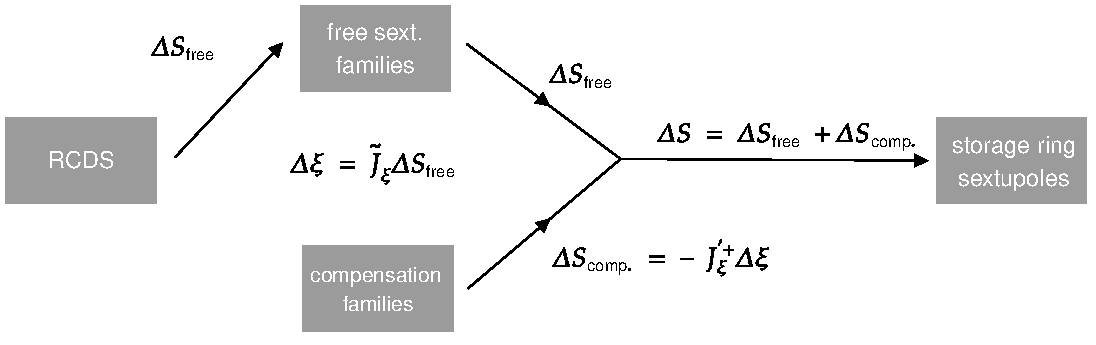
\includegraphics[width=\textwidth]{Images/compensation_scheme.pdf}
    \caption[Illustration of the compensation scheme for changing sextupole strengths with no change in chromaticity.]{Illustration of the compensation scheme for changing sextupole strengths with no change in chromaticity.}
    \label{fig:compensation}
\end{figure}
\subsubsection{Jacobian null space knobs scheme}
\label{subsubsec:nullspace}
Here the idea is to identify the combination of sextupole families living in the null space, or kernel, of the chromaticity Jacobian matrix. That is, we are interested in the set of vectors $\text{ker}(\vb{J}_\xi)=\text{span}\{\vb{s}_i\in\mathbb{R}^{21}| \vb{J}_{\xi} \vb{s}_i = \vb{0}\}_{i=1,\dots,19}$. If we perform changes along such subspace $\Delta \vb{S}\in\text{ker}(\vb{J}_\xi)$ then the resulting changes in chromaticity are null.

The reason why we can anticipate the dimension of the null space is 19 is because it contains the 6 achromatic sextupole families plus 13 degrees of freedom out of the 15 achromatic families, since at least 2 degrees of freedom are needed to act over chromaticity.

A straightforward way to identify the null space of the Jacobian is to calculate its full singular value decomposition (SVD), which expresses the Jacobian as the product
\begin{equation}
    \begin{aligned}
        \vb{J}_\xi &= \vb{U}\boldsymbol{\Sigma}\vb{V}^\intercal\\
                   &= \underbrace{\mqty[\vdots & \vdots \\
                            \vb{u}_1 & \vb{u}_2\\
                            \vdots & \vdots]}_{2\times 2}
                            \underbrace{\mqty[\sigma_1 & 0 & \dots & 0\\
                                             0 & \sigma_2 & \dots & 0 ]}_{2\times21}
                            \underbrace{\mqty[
                                \dots & \vb{v}^\intercal_1 & \dots\\
                                \dots & \vb{v}^\intercal_2 & \dots\\
                                \dots & \vb{v}^\intercal_3 & \dots\\
                                      & \vdots &    \\
                                \dots & \vb{v}^\intercal_{21} & \dots\\                              ]}_{21\times21}.
    \end{aligned}
\end{equation}
Note that the singular-values matrix has only two non-vanishing singular values $\sigma_1$ and $\sigma_2$. In the sum-over-modes form of SVD, we have
\begin{equation}
    \vb{J}_\xi = \sum_{i=0}^{21}\sigma_i\vb{u}_i\vb{v}_{i}^{\intercal} = \sigma_1 \vb{u}_1\vb{v}_{1}^\intercal + \sigma_2 \vb{u}_2\vb{v}_{2}^\intercal,
\end{equation}
in which it becomes clear that we have only two independent modes or degrees of freedom for changing chromaticity, corresponding to the horizontal and vertical degrees of freedom.

Multiplication of the SVD-decomposed $\vb{J}_{\xi}$ by $\vb{V}$ gives $\vb{J}_{\xi}\vb{V} = \vb{U}\boldsymbol{\Sigma}$, which explicitly reads
\begin{equation}
    \begin{aligned}
        \vb{J}_{\xi}\vb{v}_i & = \sigma_i \vb{u}_i, \quad i=1,2,\\
        \vb{J}_{\xi}\vb{v}_i & = \vb{0}, \quad i=3,\dots,21.\\
    \end{aligned}
\end{equation}
Revealing the sextupole strength vectors living in the null space of the Jacobian. They must be the ones associated with the vanishing singular values: $\text{ker}(\vb{J}_\xi) = \text{span}\{\vb{v}_i\}_{i=3,\dots,21}$.
%  Referring to our previous notation, we can say $\text{ker}(\vb{J}_\xi) = \text{span}\{\vb{s}_i = \vb{v}_{i+2}\}_{i=1,\dots,19}$.
Figure~\ref{fig:chrom_jac_subspaces} illustrates the fundamental subspaces associated with the chromaticity jacobian. The range of the matrix, or column space, is the chromaticity changes space. Vectors living in the null space are the sextupole strengths combinations mapped to the chromaticity space origin.

\begin{figure}
    \centering
    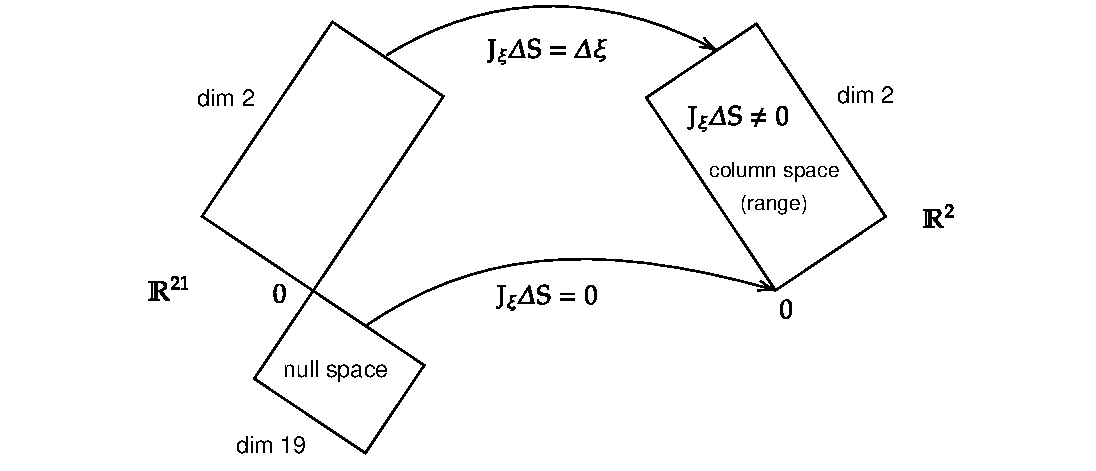
\includegraphics[width=0.8\textwidth]{Images/chrom_jacobian_subspaces.pdf}
    \caption[Illustration of chromaticity jacobian $\vb{J}_{\xi}$ fundamental subspaces]{Illustration of chromaticity jacobian $\vb{J}_{\xi}$ fundamental subspaces. The idea is to use sextupole combinations living in the null space, since these are mapped to the zero vector on the chromaticity space.}
    \label{fig:chrom_jac_subspaces}
\end{figure}

As mentioned previously, additional constraints on the families strengths variations  have been imposed to further reduce the dimensionality of the search space. In such cases, the jacobian is recalculated considering the imposed constraints. For instance, in one of the experiments the following constraints were imposed:
\begin{itemize}
    \item Families SFP1 and SFB1 were kept constant, i.e., were not allowed to change. As mentioned, they operate close to their saturation, nonlinear regime, and one cannot trust they would be able to provide reproducible magnetic field changes. Deciding not using them already reduces from 21 to 19 degrees of freedom.
    \item The pair of families SDB1 \& SDP1, SDB2 \& SDP2, SFB2 \& SFP2, SDB3 \& SDP3 were constrained to change by the same amount, starting from their respective initial strengths. This reduces the available options from 19 to 15 families.
\end{itemize}
These 15 families consist on the combination of the 6 achromatic families, the 4 pairs of constrained families and 5 other non-constrained families SDA1, SFA1, SDA2 , SFA2, and SDA3.
% The 9-dimensional chromatic space Jacobian is calculated and its null space basis reveals the 7-dimensional space spanned by the linear combination of sextupole strengths that will not change chromaticity when varied. Combining the 7-dimensional null space with achromatic families results in a 13-dimensional search space. We shall refer to such constraint configuration as \textbf{Constraint Scheme I}, to distinguish it from \textbf{Constraints Scheme II}, which consists on
Calculating the null space of the Jacobian results in a 13-dimensional search space. We shall refer to such constraint configuration as \textbf{Constraint Scheme I}, to distinguish it from \textbf{Constraint Scheme II}, which consists on

\begin{itemize}
    \item Families SFP1 and SFB1 were kept constant, by the same reason as in the previous scheme.
    \item No pair-wise constraints were imposed to the sextupole families. So, in principle, there were 19 possible families: 21 minus the two families not used.
\end{itemize}
Calculating the Jacobian null space revealed the 17 chromaticity-preserving free knobs.

% With the presentation of experimental procedures, setup and the available diagnostics, we can move on to reporting the experiments and their results. This is the focus of the next chapter.
% \subsection{Characterization of Sextupole Magnets Configurations}
% Once a configuration of sextupoles (position in parameter space) is found, the nonlinear optics it provides the machine needs to be characterized. The characterizations consisted on evaluatig/measuring the followint figures of merit and desired features
% \begin{itemize}
%     \item Injection efficiency in nominal off-axis conditions : this is the most desired characteristic. The sextupoles are to be optimized so the DA and the off-axis injection efficiency increase.
%     \item Beam Kick resilience: a small current of $2~\unit{\milli\ampere}$, concentrated in a single bucket is stored in the ring. The beam is kicked by the horizontal dipole kicker, which instantly provides a dipolar perturbation leading the beam to be displaced in the horizontal direction. The current before and after the kick is recorded by a current monitor (DCCT) and allows for the calculation of the fraction of the beam lost as a consequence of the kick and the transverse displacement. The procedure is repeated with progressively stronger kicks, and a curve of beam loss as a function of the kick can be constructed. The smaller the losses for larger kicks, the larger the resilience.
%     \item Phase portrait area: it is expected that the optimzation procedure increases the dynamic aperture of the machine, meaning it can accomodate larger oscillations and larger phase portraits $x-x^\prime$. Using beam position monitors (BPMs) at the two ends of a straight section, which record the positions of the beam centroid at each turn, we can calculate the position and angle of the beam in the middle of the straight section, and thus recostruct the phase-portrait from turn-by-turn (TbT) data.
%     \item Beam lifetime: the lifetime at SIRIUS is dominated by losses due to electron-electron interactions leading to momentum transfers exceeding the energy/momentum acceptance (MA). Optimization of DA does not necessarily leads to improvements in the MA. If the MA is reduced, the rate at which the beam is lost can increase, reducing the total lifetime. It is desireble that the configurations found during DA otpimzation do not worsen the MA and beam lifetime considerably.
%     % One dominat effect leading to beam loss is the so-called Touschek Effect, consisiting on collisions between electrons of the same bunch leading to momentum trasfers from the transverse to the longitudinal direction that can exceed the lattice tolerance to momentum deviations, the Momentum Acceptance. Momentum acceptance is the dynamic aperture for off-energy particles. Optimization of DA, which is accesed by the aforementioned objective functions, not necessarily leads to improvements in the MA. If the MA is reduced, the rate of Touschek events increases and thus the lifetime is reduced. Therefore, another desired feature from a good sextupole configurations is having a good beam lifetime. We expect not the worsen the lifetime.
%     \item Chromaticity: Sextupoles are introduced in the storage ring for correction of focusing chromatic aberretions. When changing the sextupole settings, it is desired to do so in such a manner that the chromaticity is unchanged. The methods for choosing the optimization knobs already take into account the need for keeping constant chromaticity. Still, after optimization is performed, we need to check whether chromaticity is unchanged.
% \end{itemize}
% The first two characterizations are quite similar to the two most immediate objective function candidates mentioned above. Indeed, in most nonlinear dynamics optimzation experiments, optimization using injection efficiency or kick resilience as objectives seemed to be completely interchangable. Improvements in injection efficiency necessarily led to improvements in kick resilience, and vice-versa. As shown in more details in the results section, for the SIRIUS storage ring this appears not to be the case. The configurations can be specialized to improvements solely on injection efficiency or solely to kick resilience. This feature was observed during the characterization of the optimized sextupole settings with respect to these two figures of merit.

\chapter{Experiments and Results}
\lipsum[1-10]

\chapter{Conclusions}

In this work, the Robust Conjugate Direction search algorithm (RCDS) was studied, implemented in Python and applied to the problem of optimizing the nonlinear dynamics and dynamic aperture of the SIRIUS storage ring.

The experiments focused on using injection efficiency as the objective function to examine its impact on the Dynamic Aperture (DA). While attempts were made using the beam's resilience to dipolar perturbations as the objective function, it did not yield satisfactory results in enhancing injection efficiency and ensuring repeatability across multiple injection pulses.

The optimization parameters, or knobs, were the sextupole families of the storage ring. The need to optimize dynamics while maintaining constant chromaticity imposed constraints on the selection of families or combinations of families as knobs. Two methods were considered to ensure consistent chromaticity. Additionally, we experimented with imposing supplementary symmetries on the lattice to reduce the dimensionality of the search space. Optimization proved effective irrespective of the strategy employed to preserve chromaticity and the varying dimensions of the search space.

Optimization was conducted at the machine's nominal working point, denoted as Working Point 1 (WP1), with tunes $(\nu_x, \nu_y)=(49.08, 14.14)$ and two additional working points, WP2, with tunes $(\nu_x, \nu_y)=(49.20, 14.25)$, and WP3, with tunes $(\nu_x, \nu_y)=(49.16, 14.22)$. The optimization in WP1 proved successful, yielding a sextupole configuration that achieved a remarkable $98\%$ injection efficiency. This configuration exhibited no adverse effects on chromaticity and beam lifetime, an increased phase-space area and enhanced kick resilience. In WP2, however, the optimization proved more challenging. Despite positive impacts on phase-space areas, kick resilience, and injection efficiency, the resulting efficiency of $79\%$ fell short of operational expectations. In contrast, the optimization in WP3 was deemed successful. The process not only improved phase-space areas and kick resilience but also achieved an injection efficiency of $93\%$, with no impact on lifetime and chromaticity.

The primary motivation for exploring different machine operation tunes was to elevate the fractional parts of the tunes, distancing them from integer resonances. This adjustment aimed to mitigate orbit amplification factors, which quantify the sensitivity of the orbit to perturbations. Notably, in WP3, this approach resulted in improved stability. Leveraging this new working point and recent enhancements in the orbit feedback systems, the machine achieved a world-record orbit stability. Specifically, the horizontal orbit variation is now less than $1\%$ of the horizontal beam size, and the vertical orbit exhibits variations less than $4\%$ of the vertical beam size, on average.

In conclusion, this study highlights the success of online optimization of nonlinear dynamics using RCDS in 4th-generation storage rings, exemplified by SIRIUS with its large parameter space. The outcomes of this work not serve as a benchmark for the effectiveness of the RCDS method and advocate for the inclusion and planning of online optimization routines as a standard tools during the commissioning of future 4th-generation projects.


\bibliographystyle{naturemag}
\bibliography{Chapters/Bibliografia}

\appendix
\chapter{Algorithms pseudocode}
\label{chap:pseudocode}
This appendix presents pseudocode for simplified versions of the routines implemented Python during the execution of this work. The code has been simplified for pedagogic reasons, focusing on the main characteristics of each routine composing the RCDS algortihm. In particular, checking of data consistency and adequacy are not included. The bracketing and linescan routines are presented only for the simpler case of a single parameter (knob) optimization.
\section{RCDS Bracketing}
Given the initial point $x_0$, the initial value for the objective function $f_0 = f(x_0)$, and the initial step size, the bracketing routine scans "downhill" until the function stops decreasing and starts to increase by more than the $3\sigma$ threshold. The step size is increased at each evaluation by the golden ratio $\phi=\frac{1+\sqrt{5}}{2}$, as long as it does not exceed $0.10$. The use of the golden ratio is inspired by the Golden Section Search bracket routine \cite[sec. 10.2]{press_numerical_2007}. The bracketing function returns a list of $x$ positions, which are the brackets, and the objective function evaluated at those points. Pseudocode is shown in Algorithm~\ref{alg:brackets}. The bracketing function calls the externally defined function "ObjectiveFunction()", which implements the evaluation of the figure of merit. This function increases the global variable "n\_evals" whenever it is called. This keeps track of the number of objective function evaluations, which is essential as a stopping condition for Poweel's loop.

\begin{algorithm}
    \caption{RCDS bracketing}\label{alg:brackets}
    \begin{algorithmic}[1]
    \Function{BracketingMin}{$x_0$, $f_0$, step}
        \State positions $\gets$ list containing $x_0$
        \State functions $\gets$ list containing $f_0$
        \State $x_{\text{min}}$, $f_{\text{min}}$ $\gets$ $x_0$, $f_0$
        \State dir $\gets$ $+x$
        \Comment{scan in the positive direction}
        \State $f$ $\gets$ ObjectiveFunction($x_0$ + step)
        \If{$f<f_{\text{min}}$}
            \State $f_{\text{min}}\gets f$
        \EndIf
        \State append $x_0 + \text{step}$ to positions
        \State append $f$ to functions
        \While{$f<f_{\text{min}} + 3 \sigma$}:
            \If{$|\text{step}|<0.1$}
                \State step $\gets$ step $\times$ (1 + $\phi$)
            \ElsIf{$\text{dir} = +x$}
                \State step $\gets$ step + 0.1
            \Else
                \State step $\gets$ step - 0.1
            \EndIf
            \State $f$ $\gets$ ObjectiveFunction($x_0 + \text{step}$)
            \If{$f$ is NaN}
                \State \textbf{break}
            \EndIf
            \If{$f<f_{\text{min}}$}
                \State $x_{\text{min}} \gets$ $x_0 + \text{step}$
                \State $f_{\text{min}}\gets f$
            \EndIf
            \State append $x_0 + \text{step}$ to positions
            \State append $f$ to functions
        \EndWhile
        \If{$f_0\leq f_{\text{min}} + 3 \sigma$}
        \Comment{if false, no need to scan in the other direction}
            \State dir $\gets$ $-x$
            \State step $\gets - \text{step}$
            \State start again from line 6
            \Comment{scan in the negative direction}
        \EndIf
        \State sort positions in ascending order
        \State sort the corresponding entries of functions in the same ordering as positions
        % \State subtract each entry of postions by $x_{\text{min}}$
        % \Comment{translate the origin to the minimum}
        \State \Return positions, functions, $x_{\text{min}}$, $f_{\text{min}}$
    \EndFunction
    \end{algorithmic}
    \end{algorithm}

\section{RCDS linescan}
In algortihm~\ref{alg:linescan}, the RCDS linescan function is presented. The list of positions within the brackets and measured objective functions must be provided alongside $m$, the number of points that should be sampled within the brackets, and $n$, the smallest number of points inside the brackets required for trusting the fit. Notice these are different parameters. If the provided list of positions is already of size $m$, no additional points are sampled, otherwise, additional measurements are carried out. Once $m$ points are available,  the parabola is fitted and the outilier removal routine evaluates the measured points against the model. If any outliers are removed and the remaining number of available points is smaller than $n$, this means we cannot trust the model because too little points remained, according to the user-defined value.

\begin{algorithm}
    \caption{RCDS linescan}\label{alg:linescan}
    \begin{algorithmic}[1]
    \Function{linescan}{positions, functions, $x_{\text{min}}$, $f_{\text{min}}$, $n$, $m$}
        \State $a\gets$ positions first entry
        \State $c\gets$ positions last entry
        \Comment{brackets $(a,x_{\text{min}},c)$}
        \State $V$ $\gets$ evenly spaced $m$-array w/ values $\in$ $[a, c]$
        \Comment{dense span inside the brackets}
        \State $f(V)$ $\gets$ $m$-array with NaNs
        \For{the $i$-th entry of positions}
        \Comment{reuse previously measured point}
            \State $j^*\gets \text{argmin}_{j}(|V[j] - \text{position}[i]|)$
            \State $V[j^*]\gets \text{position}[i]$
            \State $f(V)[j^*]\gets \text{functions}[i]$
        \EndFor
        \For{the $i$-th entry of $V$ which is NaN}
        \LComment{measure the points not measured yet}
            \State $f(V)$[$i$] $\gets$ ObjectiveFunction($V$[$i$])
        \EndFor
        \State $c_0$, $c_1$, $c_2$ $\gets$ CalcDeg2PolynomCoefs($V$, $f(V)$)
        \State $V$, $f(V)$ $\gets$ RemoveOutiler($V$, $f(V)$)
        \If{length($V$) $<n$ \textbf{or} $c_2\leq 0$}
        \LComment{no sufficient points for trusting the fit or wrong parabola concavity}
            \State \Return $x_{\text{min}}$, $f_{\text{min}}$
        \EndIf
        \State $V$ $\gets$ evenly spaced 1000-array w/ values $\in(a,c)$
        \State $f(V)\gets$ empty 1000-array
        \For{the $i$-th entry of $V$}
        \LComment{fine scan for min on the parabolic model}
            \State $f(V)[i] \gets$ $c_0+c_1V[i]+c_2V[i]^2$
            \Comment{$f(V)$ = [$f(a),\dots,f(c)$]}
        \EndFor
        \State $x_{\text{min}}$ $\gets V[\text{argmin}(f(V))]$
        \State $f_\text{min}$ $\gets$ min($f(V)$)
        \State \Return $x_{\text{min}}$, $f_\text{min}$
    \EndFunction
    \end{algorithmic}
    \end{algorithm}

The function references the externally defined functions "ObjectiveFunction()" "RemoveOutlier()" and "CalcDeg2PolynomCoefs()". Pseudocode for the RemoveOutlier() function is not essential here, since its implementation is simple and offers small pedagogic value for our purpose. The reader may check our python implementation of  the "remove outlier" function in the "RCDSParams" class of the "rcds.py" file of the "apsuite" repository. The conceptual idea of the routine is:
\begin{enumerate}
    \item calculate the errors as the differences between observed and fitted values.
    \item sort the errors and compute the differences between consecutive errors.
    \item if there are less than 5 points evaluated within the brackets, check if the largest and smallest differences are greater than a threshold $3\sigma$. If yes, exclude the corresponding points.
    \item calculate the avrage of the errors differences (errors standard deviation) within a specified percentile range. Identify outliers based on differences exceeding a threshold $3\sigma$ for both larger and smaller differences. Create a boolean mask to mark outliers and return the filtered array of $x$ positions and objective function measurements.
\end{enumerate}

The "CalcDeg2PolynomCoefs()" function implements the parabolic fit within the brackets and returs the zeroth, first and second degree coefficients $c_0, c_1, c_2$ for which the polynomial $c_0 + c_1x + c_2 x^2$ best explains, in the least-squares sense, the observed data.

\section{Powell's method}
Algorithm~\ref{alg:powell} presents the pseudocode for the main loop in the optimization routine. It implements Powell's method for constructing new directions with ref's.~\cite[section 10.7]{press_numerical_2007} criteria for when to replace directions and stop the routine. Stopping conditions can be reached by the maximum number of objective function evaluations the user specifies, or according to a tolerance value for deciding when the objective has changed significantly.

Again we stress that the bracketing and linescan pseudocode presented above were significantly simplified for pedagogic reasons. In particular, 1-dimensional versions were presented, omiting the the extra steps of reducing the high-dimensional minimization problem into a 1-dimensional prolem of minimizing $g(\delta) = f(\vb{x}_0 + \delta \vb{u}_i)$ for a direction $\vb{u}_i$.

Additionaly, RCDS normalizes the knobs in the $[0, 1]$ interval, so the parameter space consists on a unit hypercube. Handling of normalization and de-normalization to evaluate the objective function is also ommited.

\begin{algorithm}
    \caption{Powell directions loop}\label{alg:powell}
    \begin{algorithmic}[1]
    \Function{Optimize}{max\_evals, search\_dirs, step, tol, $\vb{x}_0$, ortho\_threshold}
        \State max\_decrease $\gets$ 0
        \State max\_decrease\_dir $\gets$ 0
        % \State search\_dirs $\gets$ Normalize(search\_dirs)

        \State $f_0\gets$ ObjectiveFunction($\vb{x}_0$)
        \State $\vb{x}_{\text{min}}\gets \vb{x}_0$
        \State $f_{\text{min}}\gets f_0$

        \For{$i$-th direction vector $\vb{u}_i$ in search\_dirs}
            \State positions, functions, $\vb{x}_{\text{min}}$, $f_{\text{min}}\gets  $ BracketingMin($\vb{x}_0$, $f_0$, step)
            \State $\vb{x}, f \gets$ LineScan(positions, functions, $\vb{x}_{\text{min}}$, $f_{\text{min}}$)

            \If{$f_{\text{min}} - f > \text{max\_decrease}$}
                \State $ \text{max\_decrease}\gets f_{\text{min}} - f$
                \State $ \text{max\_decrease\_dir}\gets i$
            \EndIf

            \State $\vb{x}_{\text{min}}\gets \vb{x}$
            \State $f_{\text{min}}\gets f$

            \State $\vb{x}_e\gets 2 \vb{x}_{\text{min}} - \vb{x}_0$
            \Comment{define exitension point}
            \State $f_e \gets$ ObjectiveFunction($\vb{x}_e$)
            \Comment{evaluate objective at extension point}
            \State $\vb{u}_{\text{new}} \gets \frac{\vb{x}_{\text{min}}-\vb{x}_0}{|\vb{x}_{\text{min}}-\vb{x}_0|}$
            \Comment{new proposed direction}
            \State max\_dot $\gets$ 0
            \Comment{max overlap w/ all the directions}
            \For{$j$-th direction vector $\vb{u}_j$ in search\_dirs}
            \State dot = $\vb{u}_j\cdot \vb{u}_{\text{new}}$
            \If{dot > max\_dot}:
                \State max\_dot $\gets$ dot
            \EndIf
            \EndFor

            \State cond1 $\gets f_0 \leq f_e$
            \State cond2lhs $\gets 2(f_0 - 2f_{\text{min}} + f_e)(f_0 - f_{\text{min}} - \text{max\_decrease})^2$
            \State cond2rhs $\gets \text{max\_decrease}(f_e = f_0)^2$
            \State cond2 $\gets$ cond2lhs $\geq$ cond2rhs
            \If{cond1 \textbf{or} cond2}
            \LComment{Numerical Recipes conditions for direction replacement}
                \State \Output max\_decrease\_dir not replaced
            \ElsIf{max\_dot < orth\_threshold}
                \LComment{If conditions are met and new dir sufficiently orthogonal, replace}
                \State \Output replacing max\_decrease\_dir
                \State $\vb{u}_i\gets \vb{u}_{i+1}$ \textbf{for} $i=1,\dots, p-1$
                \State $\vb{u}_p\gets \vb{u}_{\text{new}}$
                \LComment{and minimize along new direction}
                \State positions, functions, $\vb{x}_{\text{min}}$, $f_{\text{min}}\gets  $ BracketingMin($\vb{x}_0$, $f_0$, step)
                \State $\vb{x}_{\text{min}}, f_{\text{min}} \gets$ LineScan(positions, functions, $\vb{x}_{\text{min}}$, $f_{\text{min}}$)
            \Else
                \State \Output max\_decrease\_dir not replaced
            \EndIf
            % \State append $\vb{x}_{\text{min}}$ to positions\_history
            % \State append ${f}_{\text{min}}$ to functions\_history
            \State cond $\gets 2 |f_0 - f_{\text{min}}|\leq \text{tol}(|f_0|  + |f_{\text{min}}|)$
            \If{cond \textbf{and} tol$>0$}
                \State\Output Stopping condition met. Exiting
                \State \textbf{break}
            \ElsIf{n\_evals > max\_evals}
                \State Maximum number of objective function evaluations reached. Exiting
                \State\textbf{break}
            \EndIf
            \State $f_0\gets f_{\text{min}}$
            \State $\vb{x}_0\gets \vb{x}_{\text{min}}$

        \EndFor
    \EndFunction
    \end{algorithmic}
    \end{algorithm}


\end{document}
